\documentclass{beamer}
%\usepackage{beamerarticle}
\usepackage{heppennames}
\usepackage{hepnicenames}
\usepackage{graphicx} 
\usepackage{multirow}
\usepackage{amsbsy,amsmath,amssymb}
\usepackage{booktabs}
\usepackage{tikz}

% ********** Styl prezentacji **********
\mode<presentation>
{
	\usetheme{Singapore}
  \setbeamercovered{transparent}
   \setbeamertemplate{footline}[frame number] 
%   \setbeamertemplate{navigation symbols}{ 
%   \insertslidenavigationsymbol
%   \insertframenavigationsymbol
%   \insertsubsectionnavigationsymbol
%   \insertsectionnavigationsymbol
%   \insertdocnavigationsymbol
%   \insertbackfindforwardnavigationsymbol
%   \hskip 0.3cm
%   %\insertframenumber / \inserttotalframenumber  % <<< frame #
%   %\insertpagenumber / \insertpresentationendpage % <<< page #
% } 
}

\usepackage[english]{babel}
\usepackage[latin1]{inputenc}

% font definitions, try \usepackage{ae} instead of the following
% three lines if you don't like this look
\usepackage{mathptmx}
\usepackage[scaled=.90]{helvet}
\usepackage{courier}


\usepackage[T1]{fontenc}

\author{S. Poss for the CERN LCD group}
\institute[CERN]{CERN}

\subject{CLICCDR}
\AtBeginSection[]
{   
{
    \usebackgroundtemplate{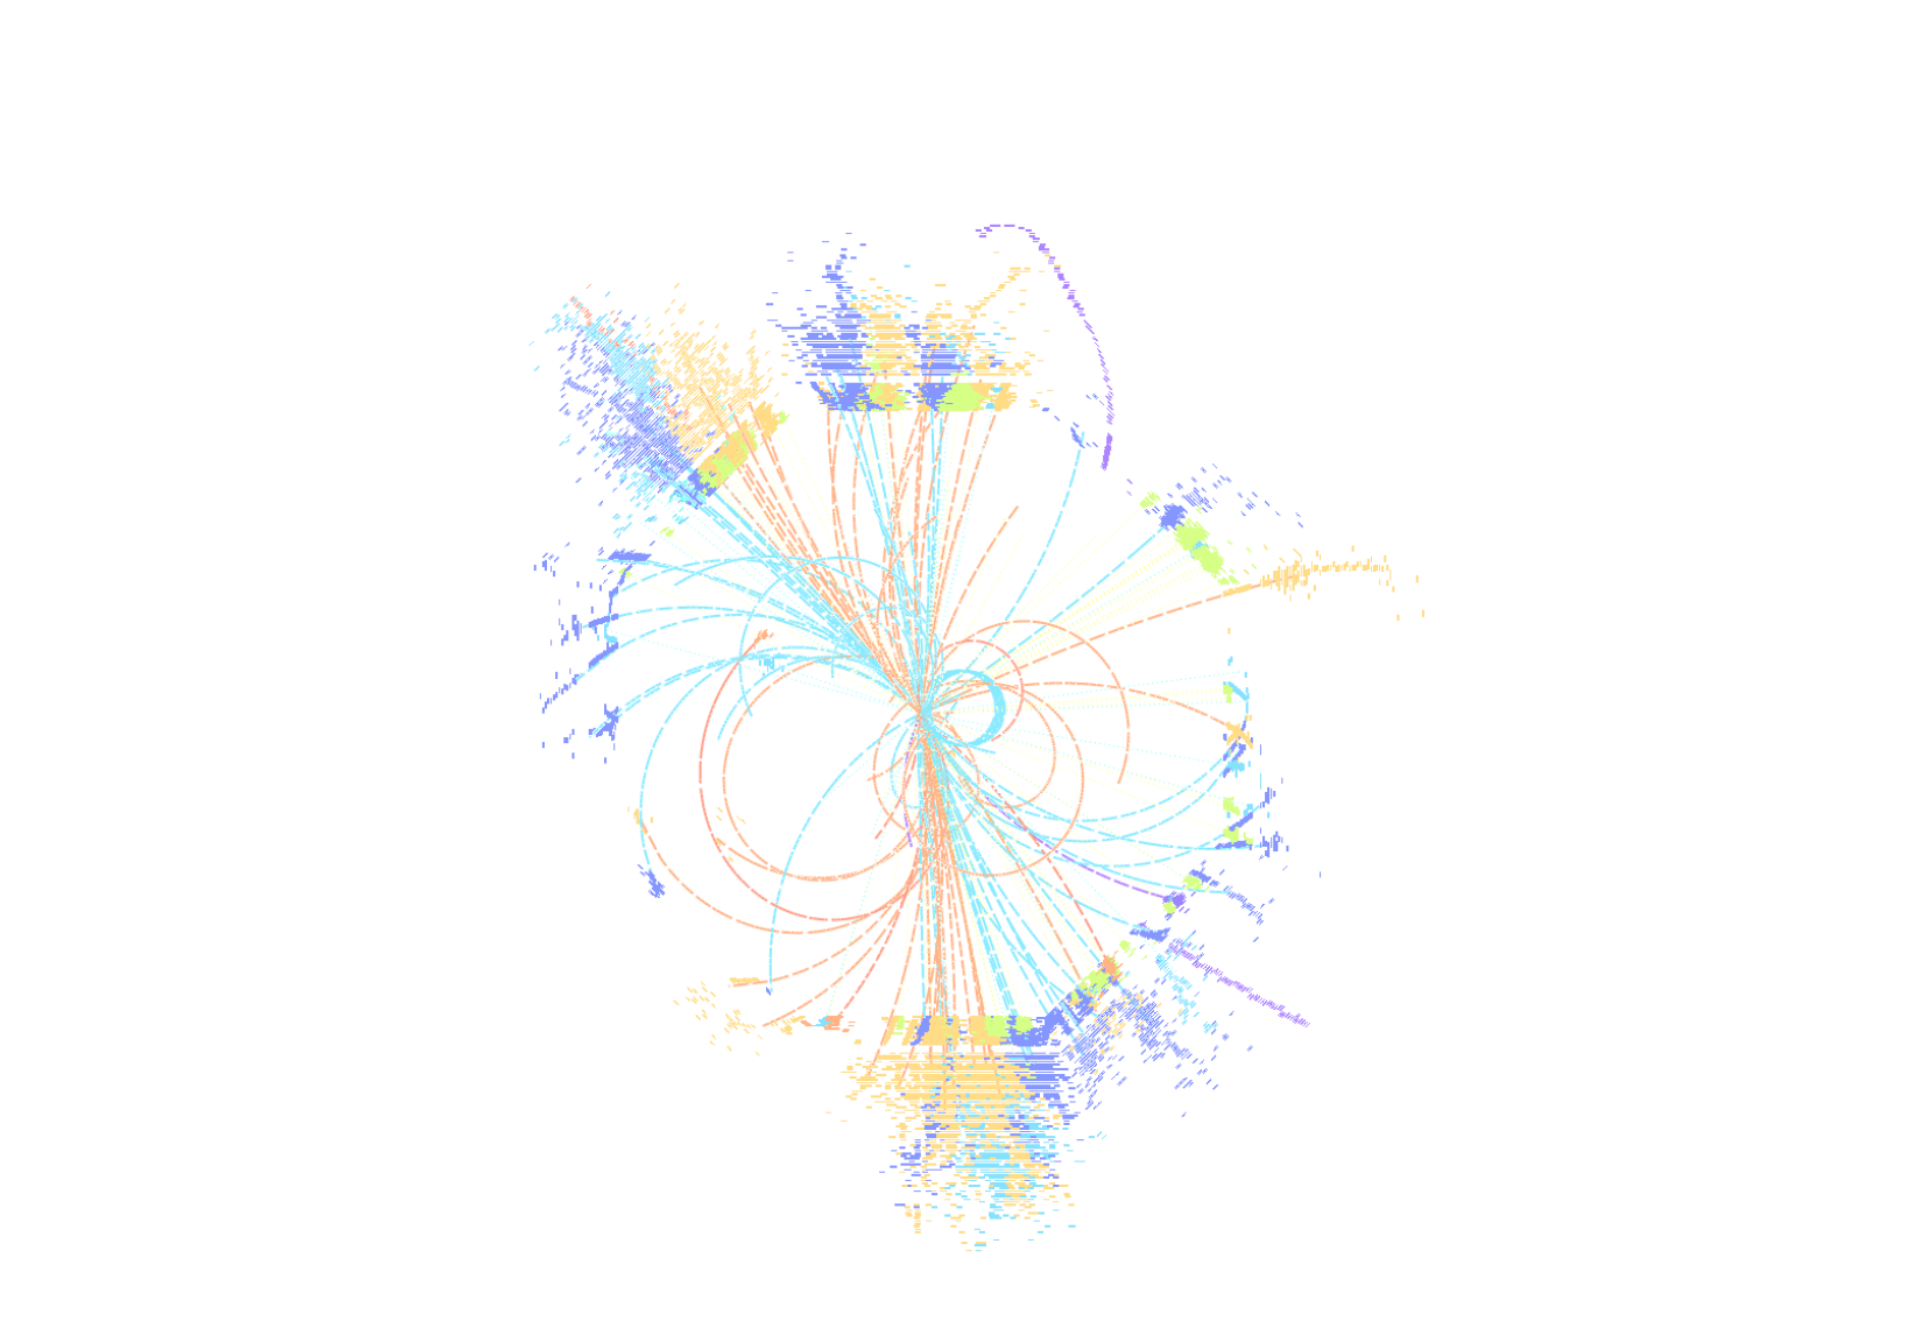
\includegraphics[width=\paperwidth]{background.png}}
	\begin{frame}<beamer>
		\frametitle{Outline}
		\tableofcontents[currentsection,currentsubsection]
	\end{frame}
}
}
\title[]{CLIC Physics and detectors CDR}
%%\subtitle{Our experience}

\date{\today}

\begin{document}

{
\usebackgroundtemplate{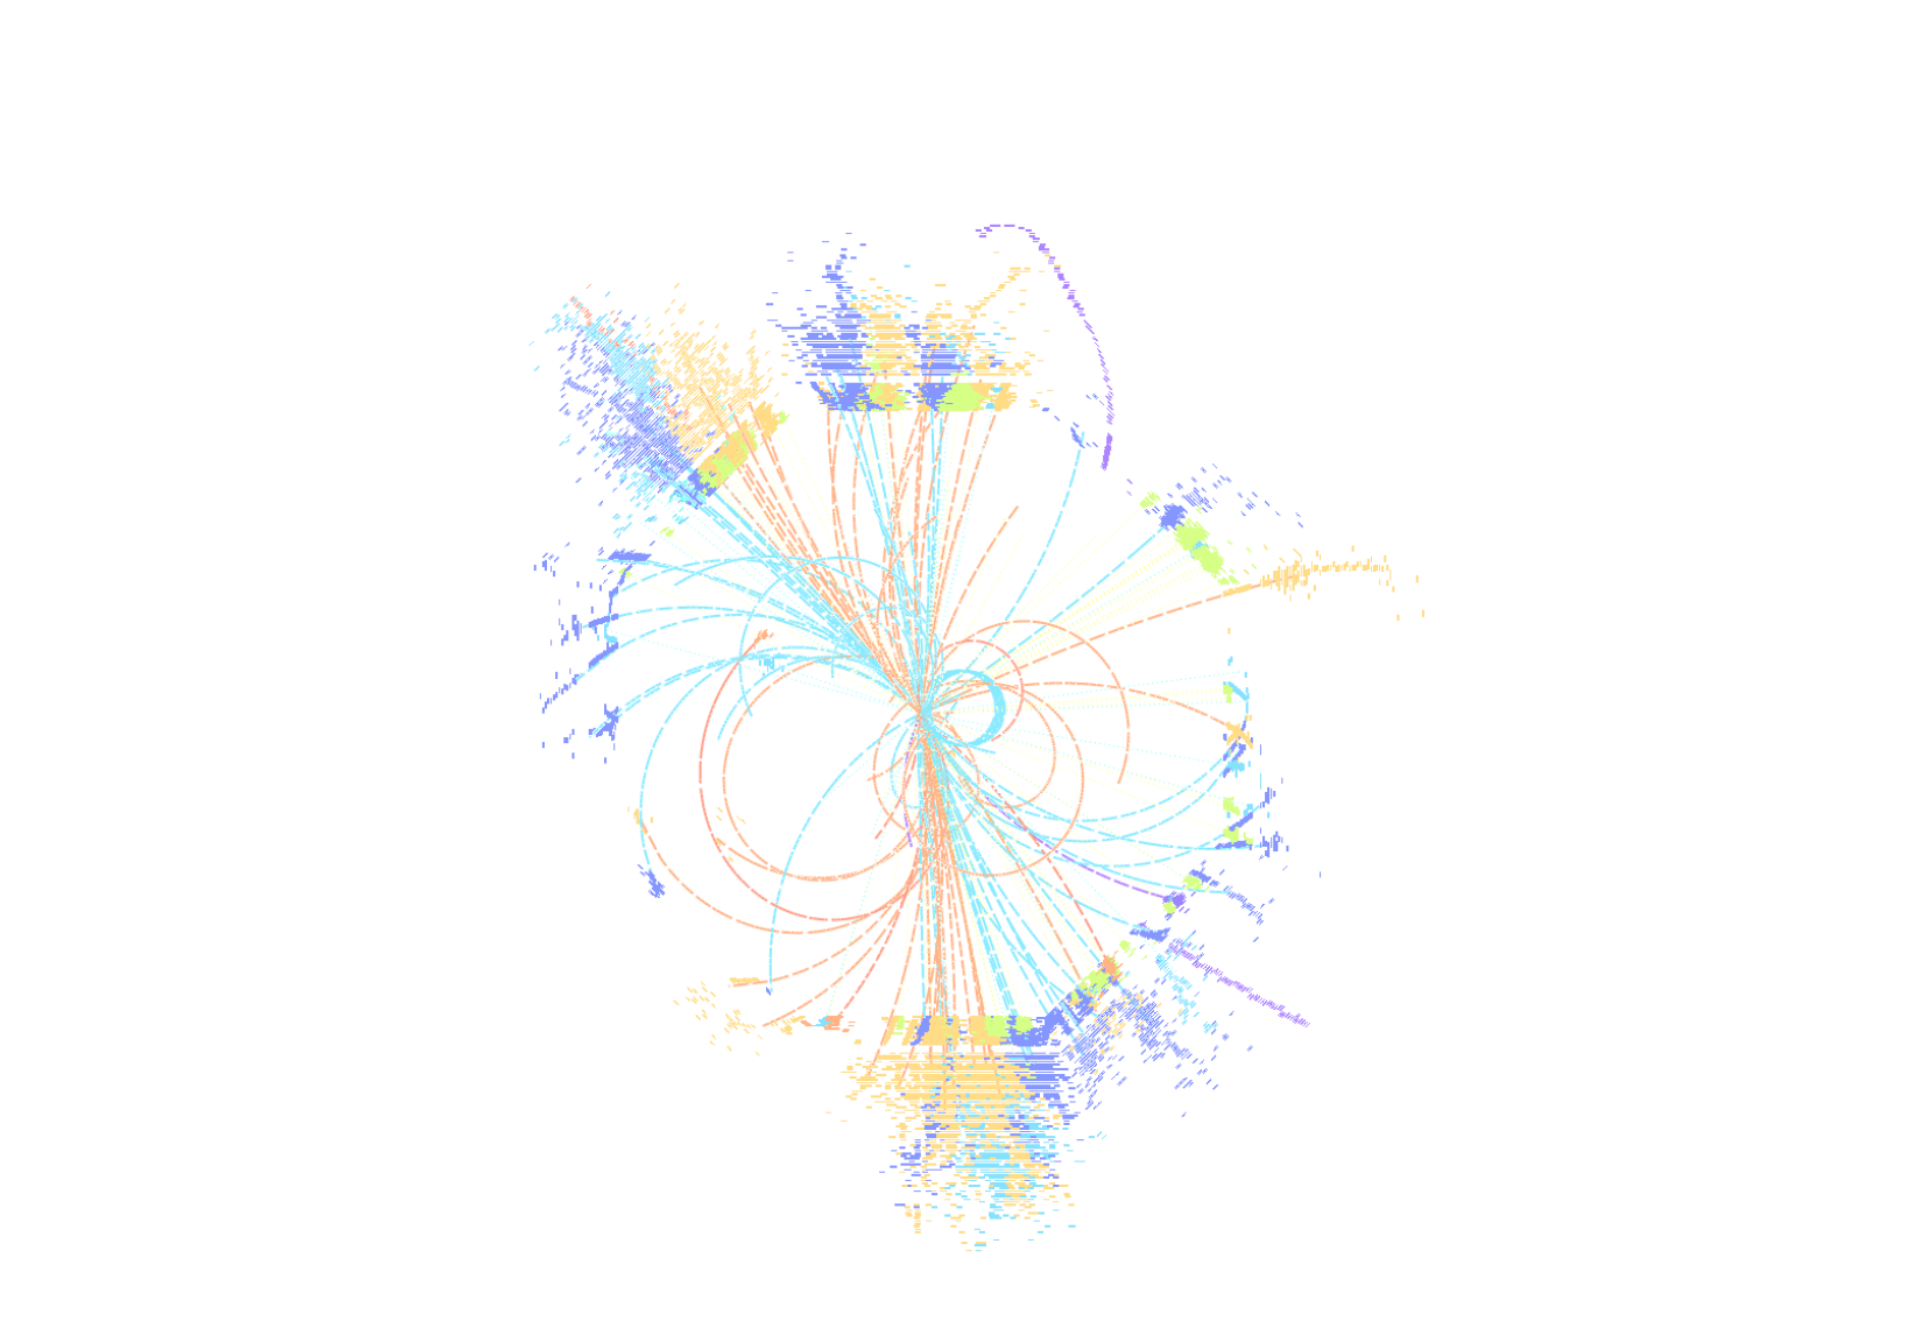
\includegraphics[width=\paperwidth]{background.png}}

\begin{frame}
	\titlepage
\end{frame}

\begin{frame}
\frametitle{Outline}
\tableofcontents
% You might wish to add the option [pausesections]
\end{frame}
}

\section[Motivations for CLIC]{Motivations for a CLIC machine}%1slide
\begin{frame}
 \frametitle{Motivations for a CLIC machine}
 CLIC: Compact LInear Collider
 \begin{itemize}
   \item $\Pep\Pem$ collisions up to $\sqrt{s}=3$TeV c.m.
   \item Machine environment challenging
\end{itemize}
~\\
CLIC physics potential:
\begin{itemize}
   \item Complementary to LHC
   \item Cleaner environment
   \item Precision Higgs physics, SUSY studies, etc.
   \item New physics beyond the LHC reach
 \end{itemize}
 
\end{frame}

\section{Physics Potential}
\begin{frame}
\frametitle{SM Higgs}
High precision measurement of its fundamental properties: mass,
total decay width, spin-parity quantum numbers, couplings to fermions and gauge bosons and
self couplings\\
\begin{columns}[c]
\column{6cm}
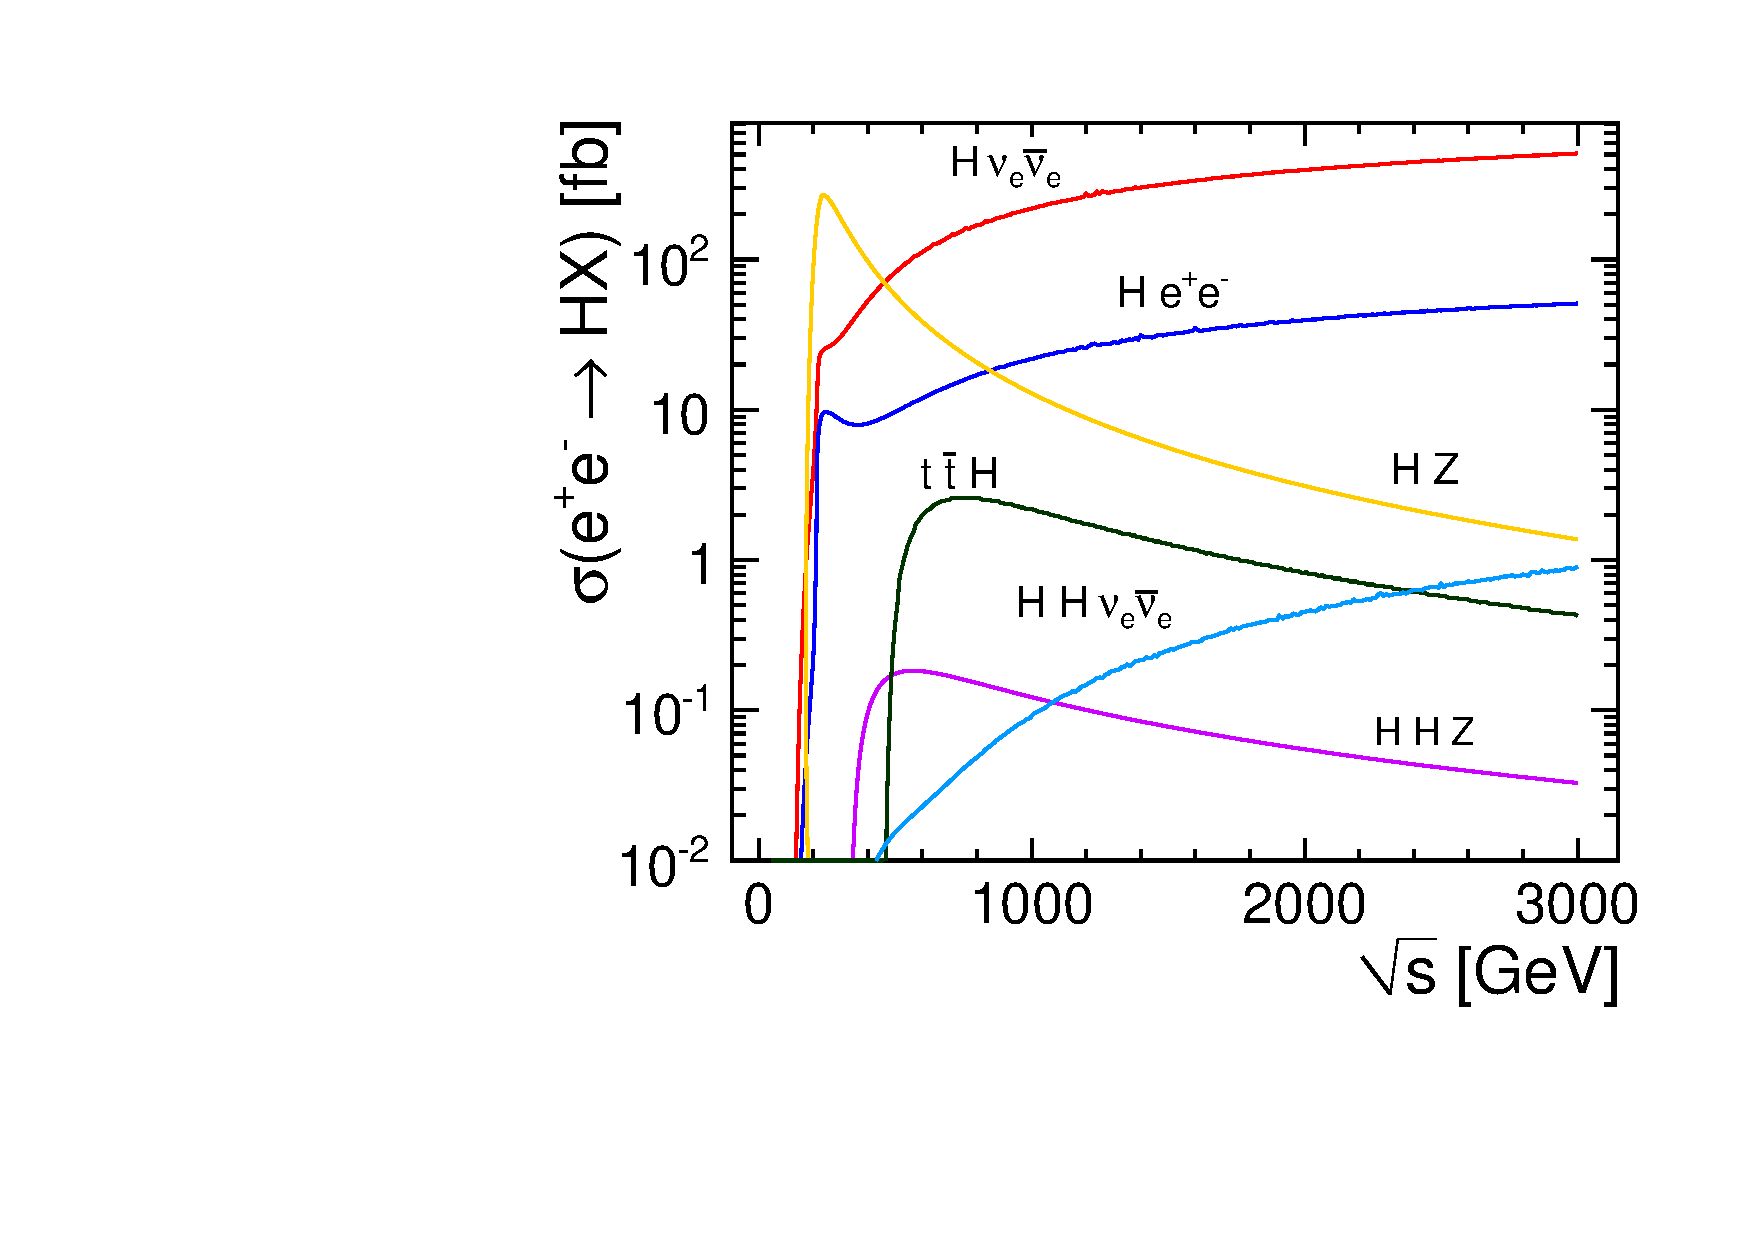
\includegraphics[width=6cm]{../SIDWorkshop/xsec_vs_cme.pdf}
\column{6cm}
\begin{center}
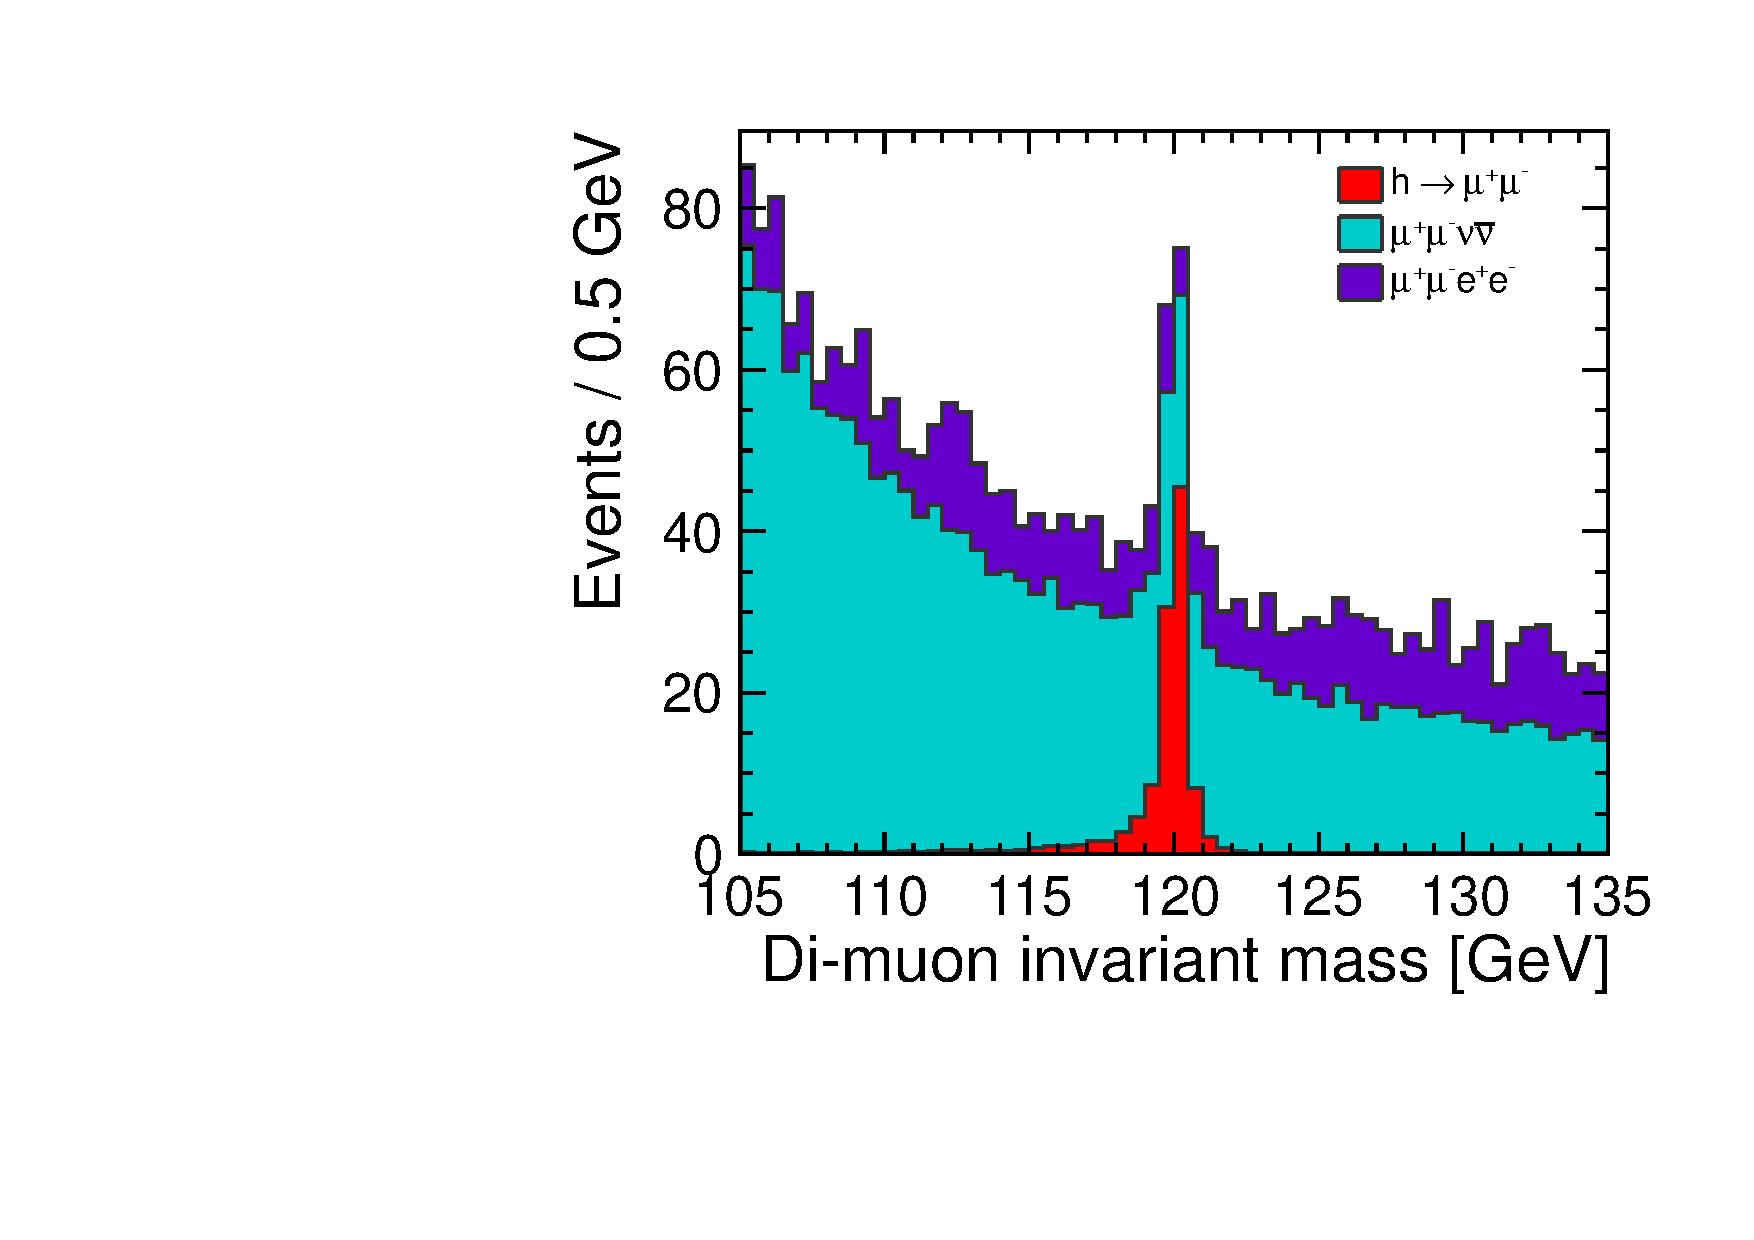
\includegraphics[width=3cm]{ee_h_mumu_mass_mh120GeV.pdf}
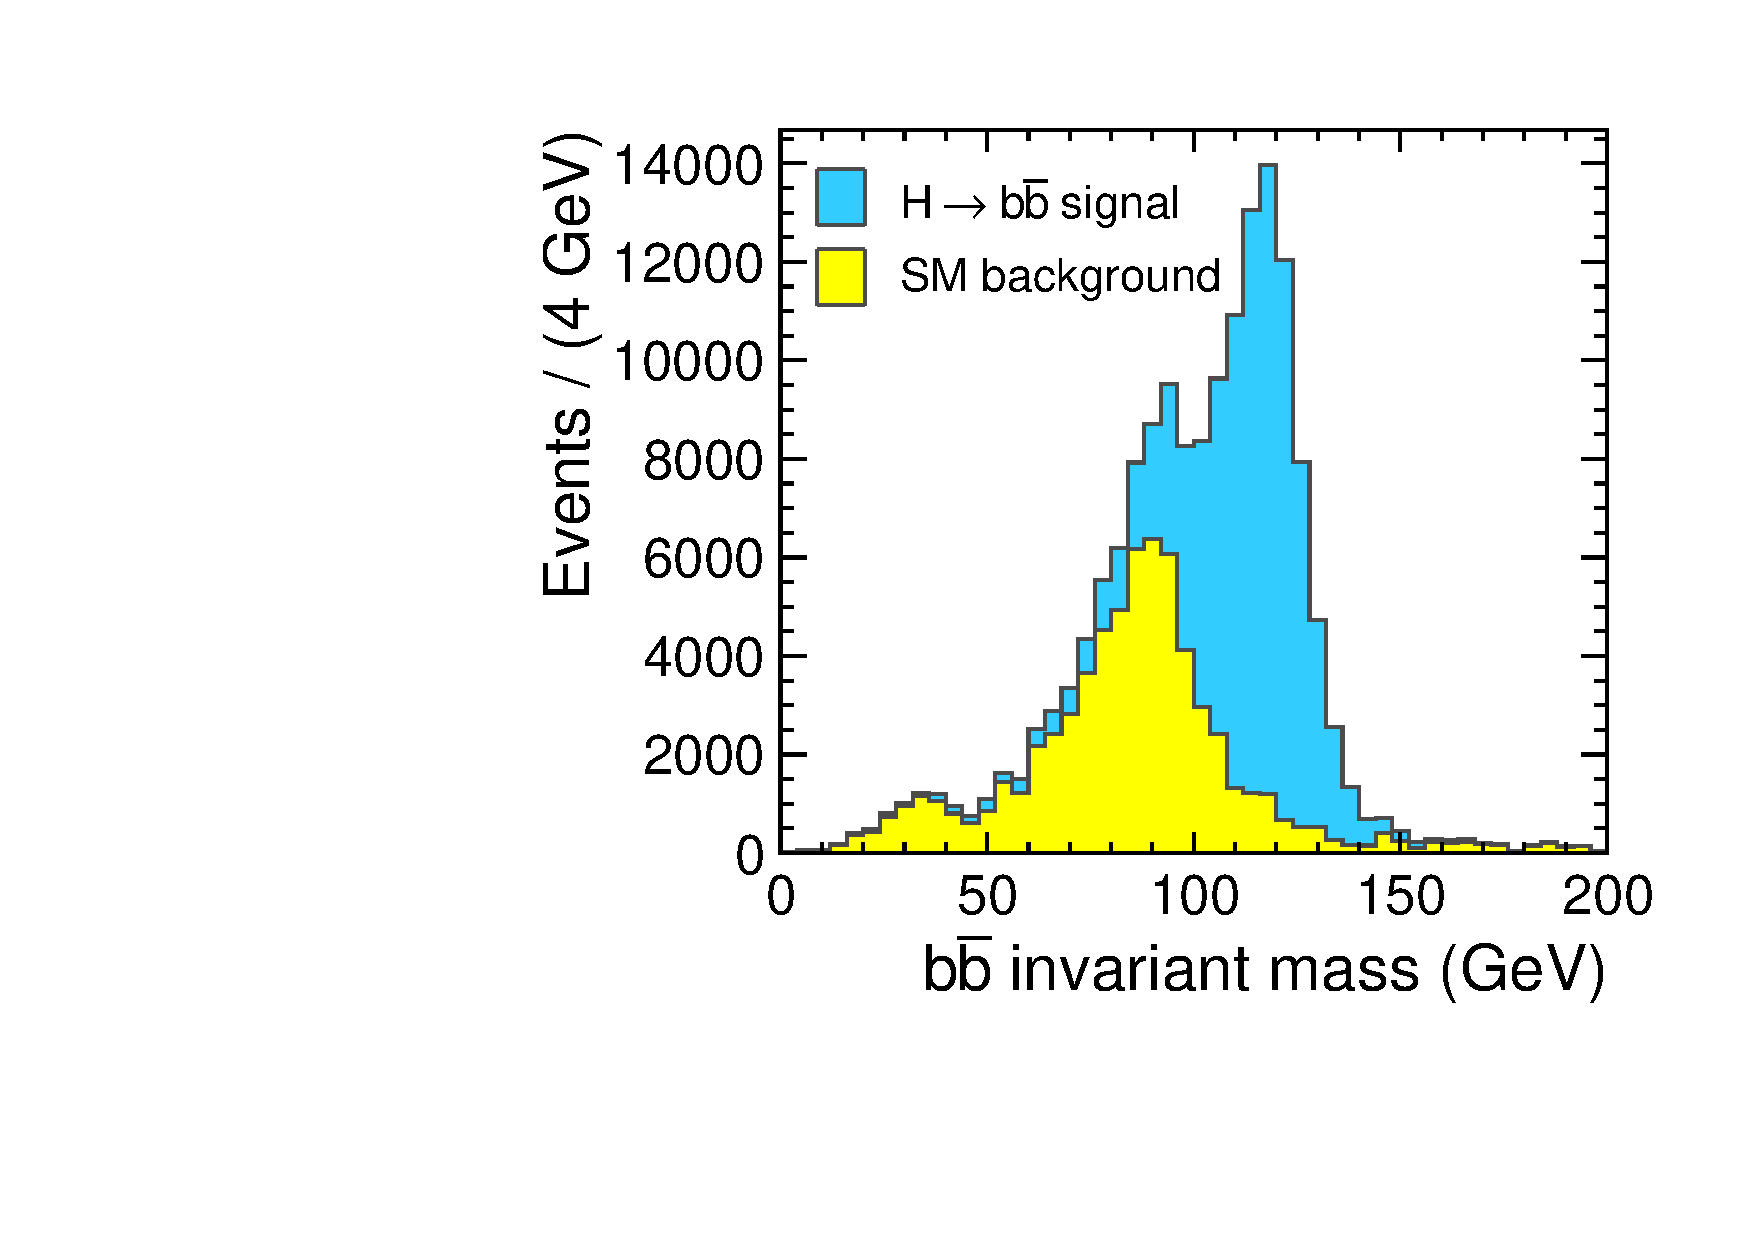
\includegraphics[width=3cm]{../SIDWorkshop/ee_h_bb_mass_mh120GeV.pdf}\\
\begin{tabular}{cc}
Coupling & precision at 3TeV\\
\midrule
$g_{\PH\to\Pbottom\APbottom}$ & 2\%\\
$g_{\PH\to\Pcharm\APcharm}$ & 3\% \\
$g_{\PH\to\mu\mu}$ & 15\%\\
\bottomrule
\end{tabular}
\end{center}
\begin{tikzpicture}[remember picture, overlay, transform shape, rotate=45,]
\node<2>[inner sep=0pt, scale=1.5] at (4.5,0.) {% 
      {\Huge \alert{More later !}}%
    };%
\end{tikzpicture}
\end{columns}
Ongoing studies for self coupling $\lambda_{HHH}$.
\end{frame}

\begin{frame}
\frametitle{BSM Higgs}
\begin{columns}[c]
\column{6cm}
$\Pep\Pem \to \PH\PA \to \Pbottom\APbottom\Pbottom\APbottom$\\
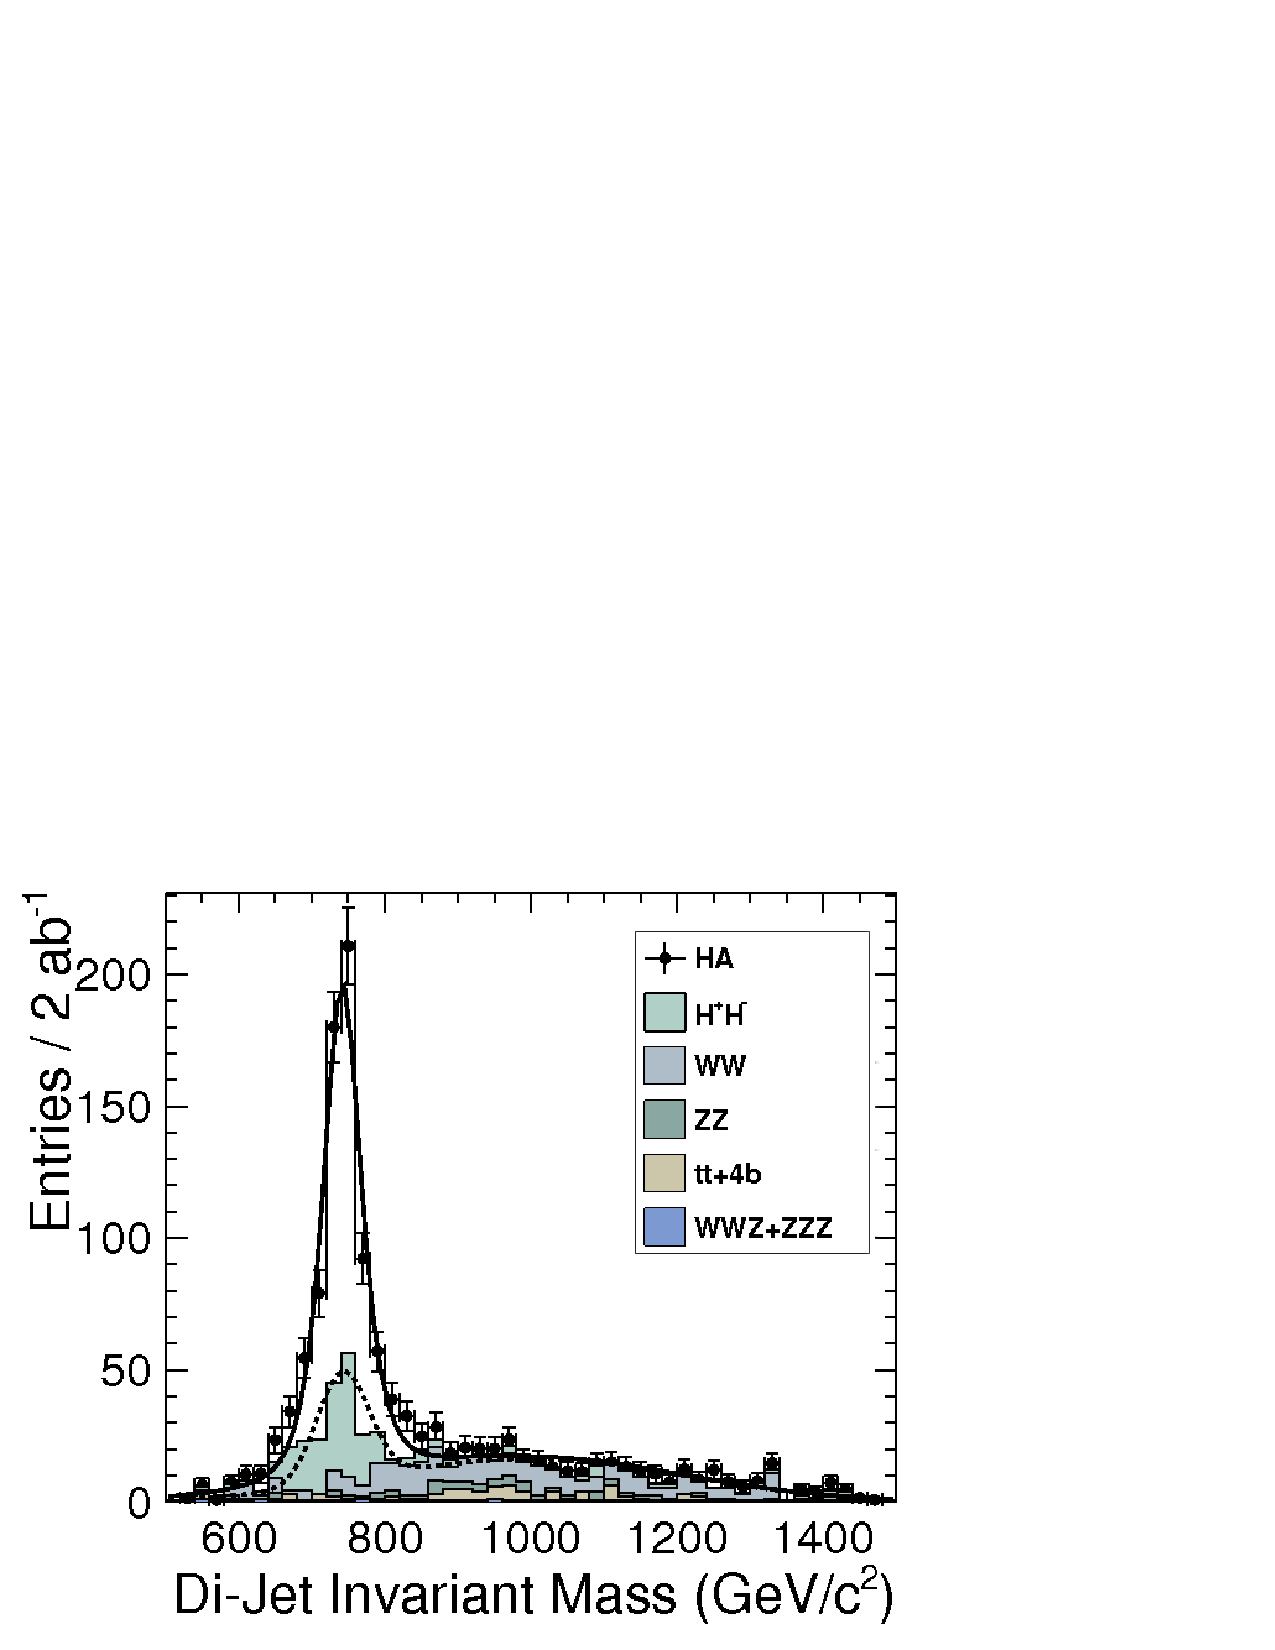
\includegraphics[width=5cm]{HAMass742_Bkg_CKFM_00BX_FJ.pdf}
\column{6cm}
$\Pep\Pem \to \PHp\PHm \to \Ptop\APbottom\APtop\Pbottom$
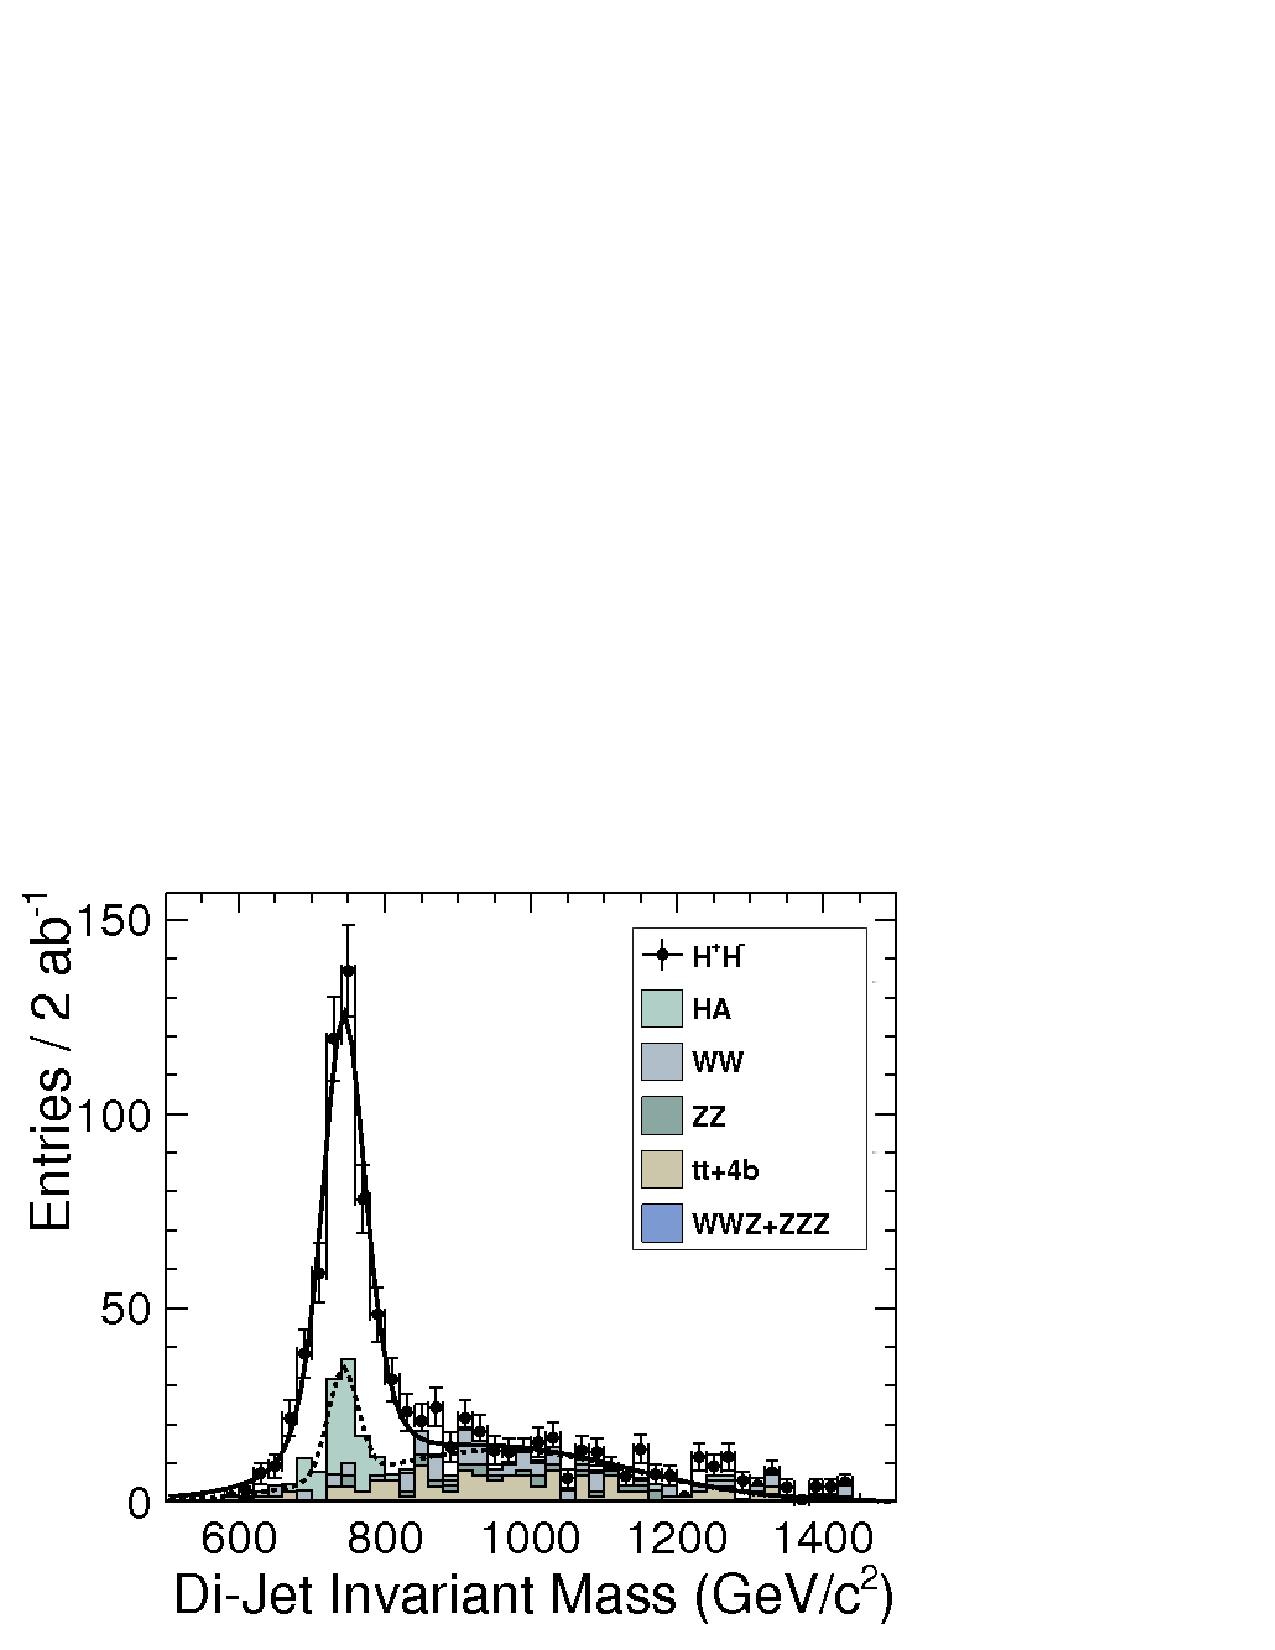
\includegraphics[width=5cm]{Hpm_Mass742_Bkg_CKFM_00BX_FJ.pdf}
\end{columns}
\begin{center}
\begin{tabular}{ccc}
\toprule
~ & $\sigma(m)/m$ & $\sigma(\Gamma)/\Gamma$\\
\midrule
$\PA/\PH$ & 0.002 & 0.10\\
$\PHpm$ & 0.005 & 0.15\\
\bottomrule
\end{tabular}
\end{center}
$\Rightarrow$ determination of $\sigma(\tan \beta)/\tan \beta <$ 0.06.
%\begin{tikzpicture}[remember picture, overlay, transform shape, rotate=45,
%scale=2] \node<2>[inner sep=0pt] at (current page.center) {%
%        {\Huge \alert{More later !}}%
%    };%
%\end{tikzpicture}
\end{frame}

\begin{frame}
\frametitle{SUSY}
\begin{center}
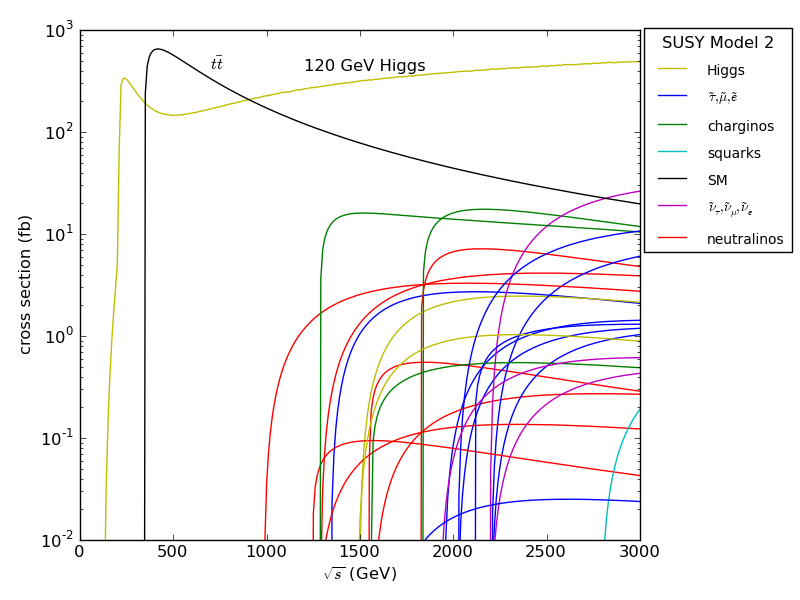
\includegraphics[width=9cm]{../SIDWorkshop/susy_model2.png}
\end{center}
Study chargino and neutralino masses by measuring kinematic endpoints of the
energy distributions, in channels like $\PSgxzii \to \Ph \PSgxzi$
\begin{tikzpicture}[remember picture, overlay, transform shape, rotate=45,
scale=2] \node<2>[inner sep=0pt] at (current page.center) {%
        {\Huge \alert{More later !}}%
    };%
\end{tikzpicture}

\end{frame}
\begin{frame}
\frametitle{SUSY}
Susy breaking models separation capability:
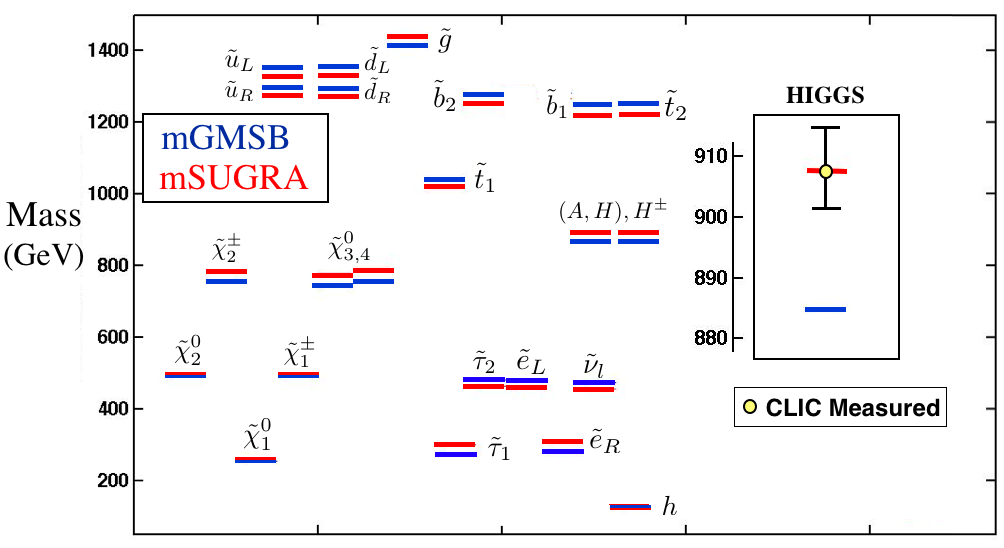
\includegraphics[width=10cm]{../SIDWorkshop/GvM.png}
\end{frame}
\begin{frame}
\frametitle{Other studies}
\begin{itemize}
  \item High scale stucture of SUSY
  \item Neutralino Dark Matter hypothesis
  \item Higgs strong interaction
  \item Z'
  \item Contact interaction
  \item Extra dimensions
\end{itemize}
\end{frame}
\begin{frame}
\frametitle{Physics potential summary}
\begin{center}
{\scriptsize
 \begin{tabular}{ ccccc }
    \toprule
 Machine &     LHC14 & SLHC & LC800 & CLIC3\\
 Luminosity & $100\textrm{fb}^{-1}$ & $1\textrm{ab}^{-1}$&
 $500\textrm{fb}^{-1}$& $1\textrm{ab}^{-1}$\\
\midrule
squarks [TeV] &   2.5 & 3 & 0.4 & 1.5 \\
sleptons [TeV] &   0.3 & - & 0.4 & 1.5 \\ 
$\textrm{Z}'$ ({\tiny SM ~couplings}) [TeV]  &  5 & 7 & 8 & 20   \\ 
%\Zprime ({\tiny SM~couplings})  &     5& 6  & 8 & 22 \\
%$q*$      &    6.5 & 7.5 & 0.8 & 3 \\
%$l*$       &   3.4 & - & 0.8 & 3 \\
2 extra dims $M_D$ [TeV]  &    9 & 12 & 5-8.5 & 20-30 \\
%$W_L W_L$      &  3.4sig& >3.4sig& -& 70sig\\
TGC (95\%)  ({\tiny \rm $\lambda_{\gamma} $~coupling}) &   0.001& 0.0006& 0.0004& 0.0001 \\
$\mu$ contact scale [TeV] &  15& - & 20 & 60 \\
Higgs compos. scale [TeV] & 5-7 & 9-12 & 45 & 60\\
    \bottomrule
  \end{tabular}
  }
 \end{center}
 CLIC can 
 \begin{itemize}
   \item extend the \alert{discovery reach} of LHC,
   \item offer the opportunity of \alert{precise measurements} of masses and
 couplings.
 \end{itemize}
\end{frame}


\section[CLIC]{The CLIC Machine}
\begin{frame}
\frametitle{CLIC machine Conceptual Design Report}
\begin{itemize}
  \item Released later in 2012
  \item Addresses the 3TeV case, the most difficult
  \item Presents the different technical aspects of a CLIC machine
  \item Details the machine properties
  \item Demonstrates (with hardware tests) the feasibility of such machine
\end{itemize}
Here: brief overview of the CLIC properties
\end{frame}
\begin{frame}
\frametitle{CLIC Technology}
\begin{columns}[c]
\column{6cm}
2 beam acceleration scheme:\\ drive beam and main beam
\begin{itemize}
  \item Gradient 100 MV/m
  \item Energy: from few-hundred GeV upgradable in steps up to 3 TeV; R\&D has
  focused on 3 TeV
\end{itemize}
\column{6cm}
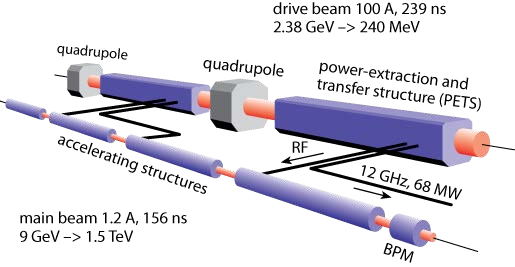
\includegraphics[width=6cm]{clicacceleration.png}
\end{columns}
\end{frame}

\begin{frame}
\frametitle{CLIC properties}
%compare to LHC/ILC
\begin{center}
\begin{tabular}{ccc}
 & CLIC 0.5TeV & CLIC 3TeV\\
 \midrule
L [$\textrm{cm}^{-2}\,\textrm{s}^{-1}$] & $2.3\times 10^{34}$&$5.9\times
10^{34}$
\\
\midrule
Bunch crossing separation  & 0.5 ns & \alert{0.5 ns}\\
\midrule
Bunch crossings per train & 354 & \alert{312}\\
\midrule
Train repetition rate  & 50 Hz & 50 Hz\\
\midrule
Crossing angle & 20mrad & 20mrad\\
\bottomrule
\end{tabular}\\
~\\
\alert{Whole bunch train in 156ns.}
\end{center}
\end{frame}
\begin{frame}
\frametitle{Machine Detector Interface}
Push-Pull system:\\
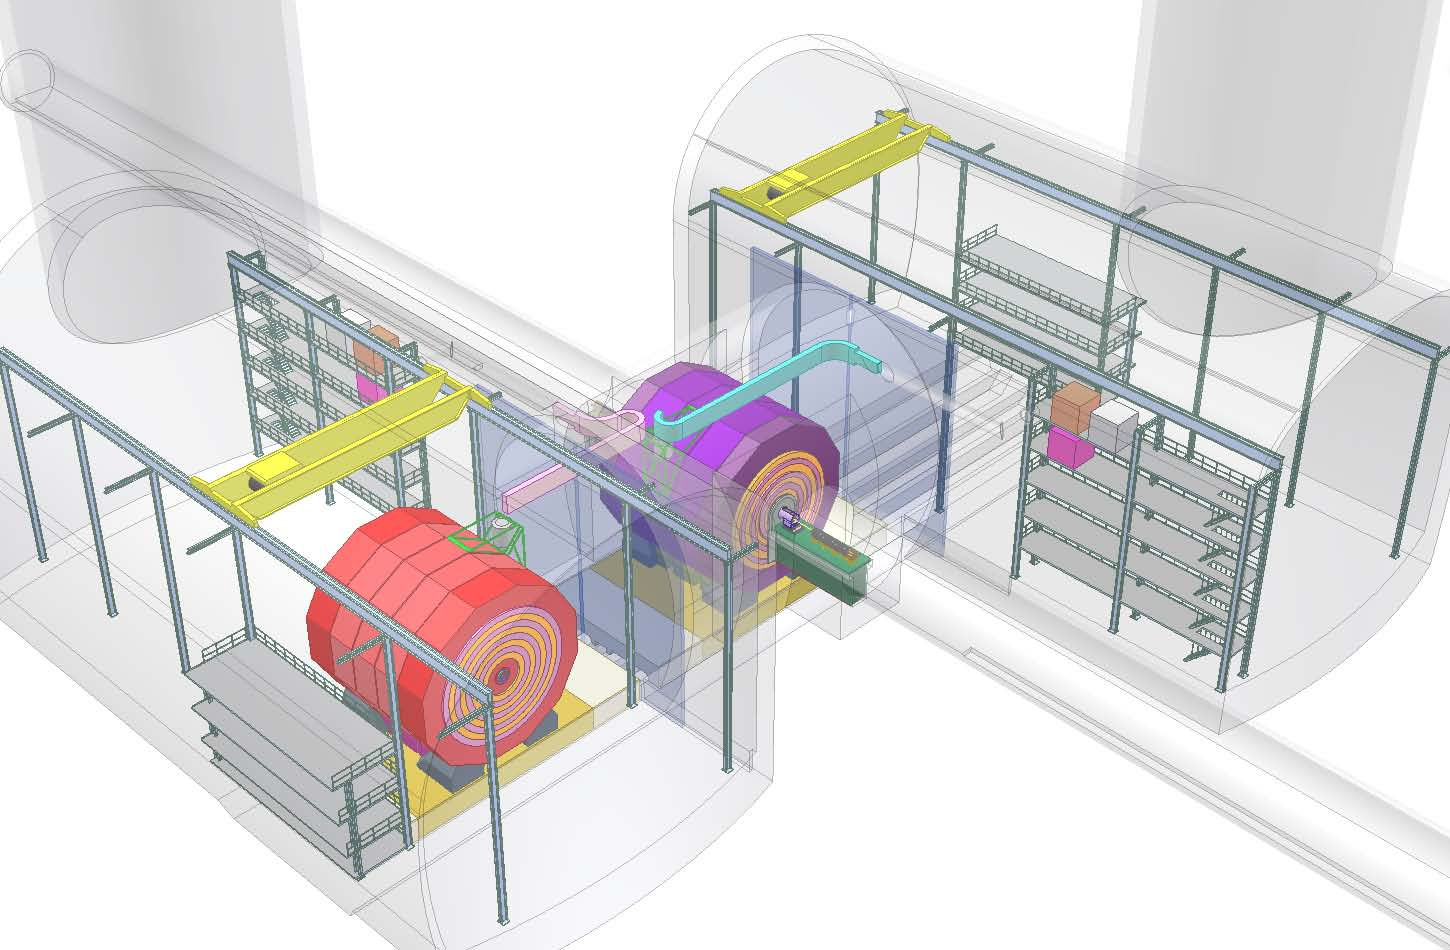
\includegraphics[width=10cm]{PushPull.png}
\end{frame}
\begin{frame}
\frametitle{Machine Detector Interface}
\begin{center}
\begin{tikzpicture}[scale=1] 
\node[] (0.0, -0.3) {\includegraphics[width=10cm,clip,trim= 0 0 0
0]{Figure_13_14.pdf}}; 
\draw<1>[<-,ultra thick, red] (-1.0,0.0)  to[] (-1.0,-3.5);
\end{tikzpicture}
\alert{Last accelerator element is IN the detector}
\end{center}
\end{frame}

\begin{frame}
\frametitle{Beam-induced backgrounds}
\begin{center}
\begin{tabular}{ccc}
 & CLIC 0.5TeV & CLIC 3TeV\\
\midrule
Nb $\gamma\gamma\to\textrm{had}$/BX & 0.2 & \alert{3.2}\\
\midrule
Nb incoherant pairs/BX & $0.8\times10^{5}$ & \alert{$3\times10^5$}\\
\midrule
Nb coherent pairs/BX & $10^2$ & $3.8\times 10^8$\\
\bottomrule
\end{tabular}
\end{center}
~\\
\alert{Very large beam-induced background rates!}\\
\begin{itemize}
  \item Coherent pairs very forward
  \item Incoherent pairs mostly forward
\end{itemize}
$\to$ impact on the very forward detectors design\\
~\\
\begin{itemize}
  \item $\gamma\gamma\to\textrm{hadrons}$ all over the detector acceptance.
\end{itemize}
\alert{Need to deal with those}
\end{frame}

\section[Detectors]{The Detectors}
\begin{frame}
\frametitle{Required performance}
\begin{itemize}
  \item Trigger less readout of full train: time stamping, multi-hit capacity,
  filtering algorithms during reconstruction
  \item High resolution pixel detector for displaced vertices identification:\\
  {\scriptsize
  \begin{tabular}{lc}
  p = 1 Gev & $\sigma_{d0}\sim20\mu m$\\
  p = 100 GeV & $\sigma_{d0}\sim5\mu m$
  \end{tabular}
  }~\\ ~\\
  \item Momentum resolution:\\
  {\scriptsize 
  $\sigma(p_{\textrm{T}})/p_{\textrm{T}}^2\sim 10^{-5}\textrm{GeV}^{-1}$
   }~\\ ~\\
  \item Good jet-energy resolution (W/Z separation)\\
  {\scriptsize 
$\sigma(E_j)/E_j = 5\%-3.5\%$ for $E_j = 50\textrm{GeV}-1\textrm{TeV}$
  }~\\ ~\\
\end{itemize}
\end{frame}
\begin{frame}
\frametitle{Particle Flow Paradigm}
Jet energy:
\begin{itemize}
  \item 60\% carried by charged particles
  \item 30\% by photons
  \item 10\% by long-lived neutral hadrons
\end{itemize}
Particle Flow: reconstruction of the \alert{4-momenta of all visible
particles}:
\begin{itemize}
  \item momenta measured in the tracking detectors for charged particles
  \item energy measured in the calorimeters for photons and neutral hadrons
\end{itemize}
$\Rightarrow$ need for \alert{high precision tracking and high granularity
calorimeters}
\end{frame}
\begin{frame}
\frametitle{Overview}
\begin{columns}[c]
\column{6cm}
\centering
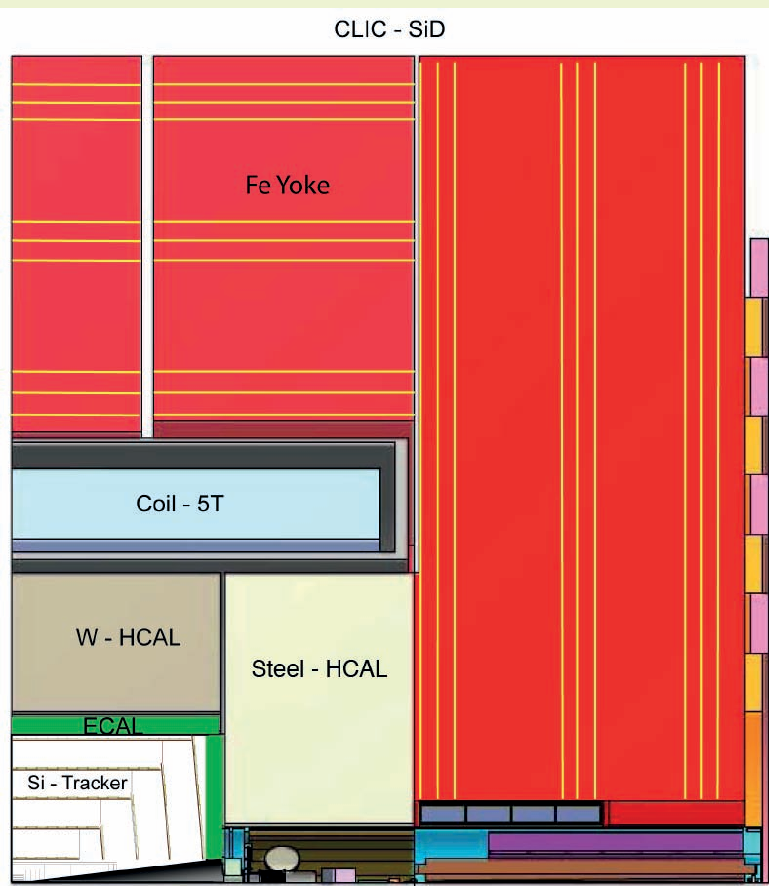
\includegraphics[width=5cm]{../SIDWorkshop/CLIC_SiD_xz.pdf}
\column{6cm}
\centering
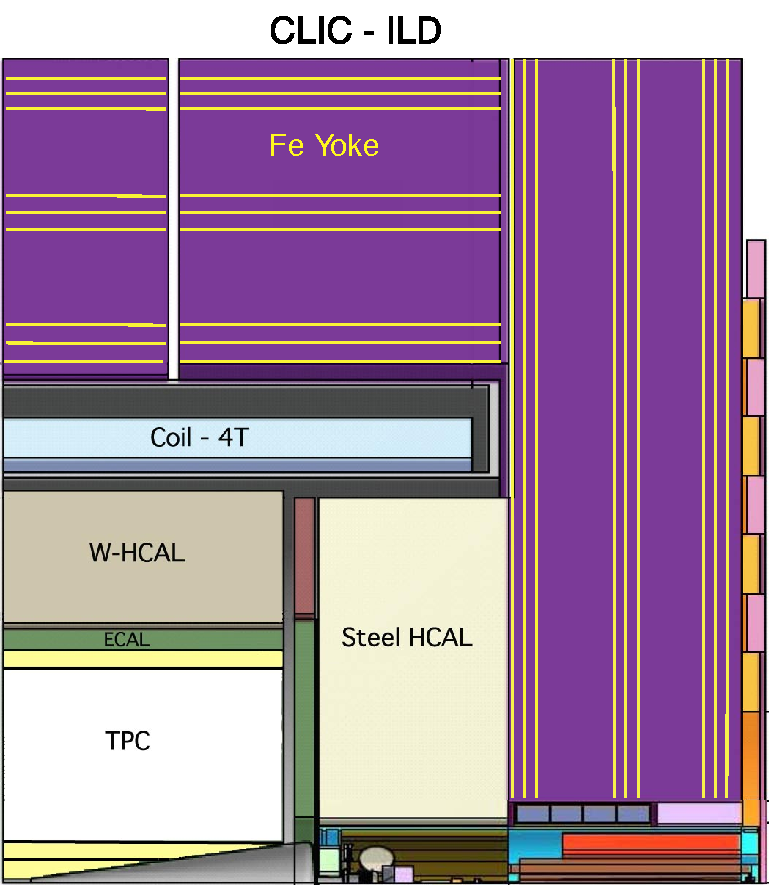
\includegraphics[width=5cm]{../SIDWorkshop/CLIC_ILD_xz.pdf}
\end{columns}
\end{frame}
\begin{frame}
\frametitle{Vertex detector optimization}
\begin{center}
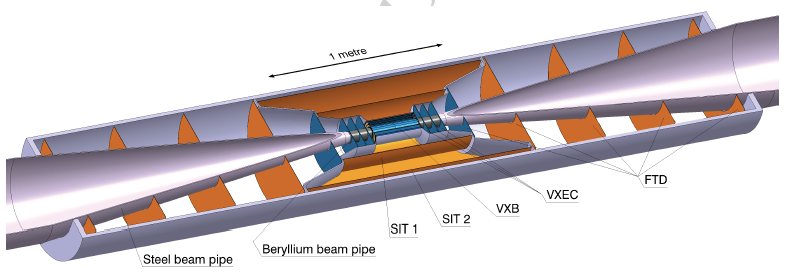
\includegraphics[width=8cm]{VertexDetector.png}
\end{center}
\begin{itemize}
  \item $20\times20\mu m$ pixel size
  \item 0.2\% X$_0$ material per layer (very thin)
  \item Time stamping 10ns
  \item Triggerless readout
  \item Radiation level $<10^{11} n_{eq}cm^{-2}year^{-1}  \Leftarrow 10^4
  \times$ lower than LHC
\end{itemize}
\alert{Challenging R\&D project}
\end{frame}

\begin{frame}
\frametitle{Tracking in CLIC\_SiD}
\begin{columns}[c]
\column{6cm}
\begin{center}
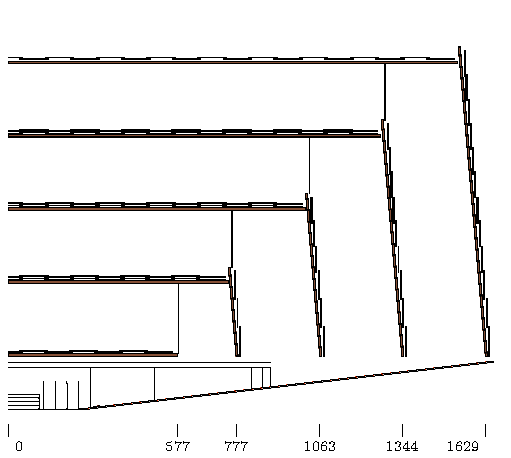
\includegraphics[width=6cm]{sid_tracker_zx.pdf}
\end{center}
\column{6cm}
\begin{itemize}
  \item All silicon tracking
  \item Efficiency ($p_{\textrm{T}}>1$GeV): $>99\%$
  \item Mom. resolution: $\sigma(\Delta(p_{\textrm{T}})/p_{\textrm{T}}^2)<
  2\cdot10^{-5}/$GeV
\end{itemize}
\alert{Compatible with requirements}\\
Hardware development to be carried out to demonstrate this.
\end{columns}
\end{frame}
\begin{frame}
\frametitle{Tracking in CLIC\_ILD}
\begin{columns}[c]
\column{6cm}
\begin{center}
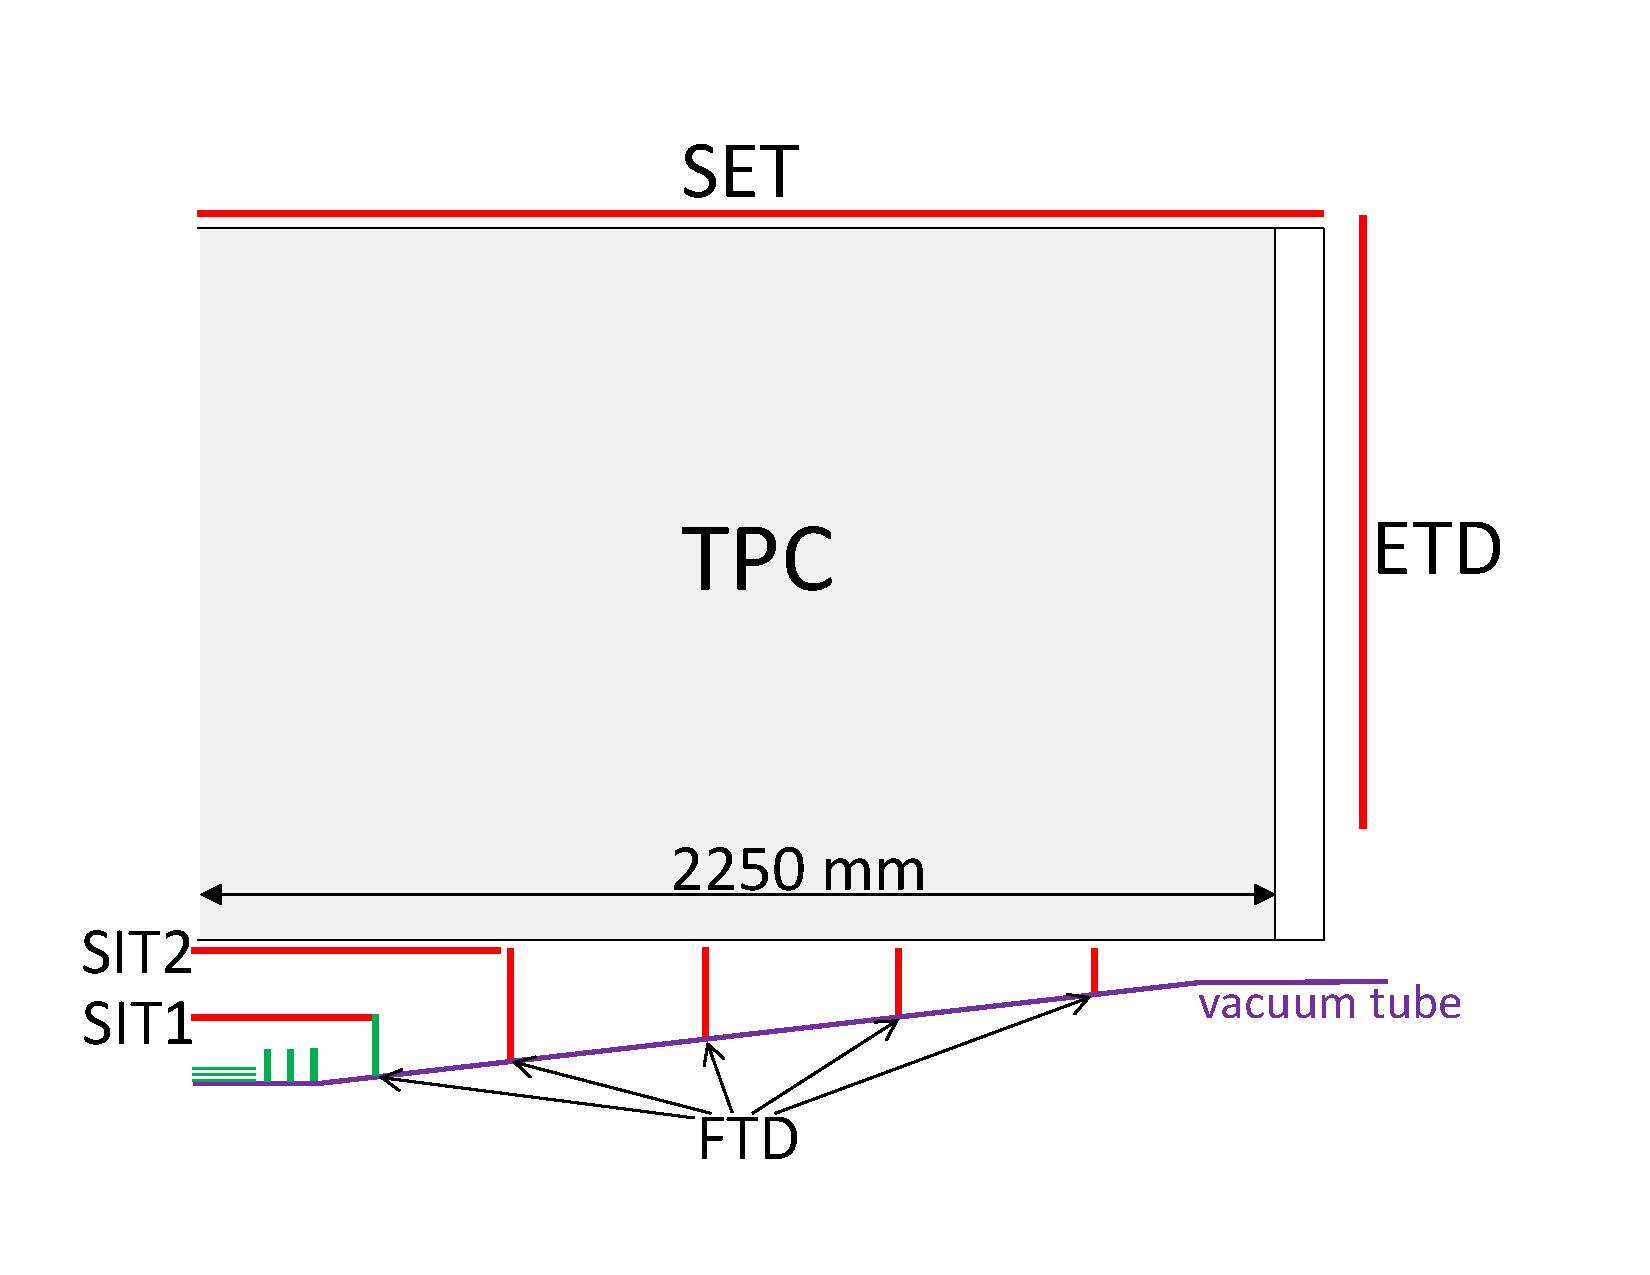
\includegraphics[width=6cm]{CLIC_ILD_tracking_geom.pdf}
\end{center}
\column{6cm}
\begin{itemize}
  \item Time Projection Chamber
  \item Completed by silicon layers
  \item Efficiency ($p_{\textrm{T}}>1$GeV): $>99\%$
  \item Mom. resolution: $\sigma(\Delta(p_{\textrm{T}})/p_{\textrm{T}}^2)\sim 2\cdot10^{-5}/$GeV
\end{itemize}
\alert{Compatible with requirements}\\
Hardware development to be carried out to demonstrate this.
\end{columns}
\end{frame}
\begin{frame}
\frametitle{ECAL}
\begin{tabular}{ccc}
    & CLIC\_ILD & CLIC\_SiD\\
\midrule
Absorber/Active element & Tungsten / Si Pads & Tungsten / Si Pads\\
\midrule
Sampling layers & $30(20\times2.1, 10\times4.2)$ & 
$30(20\times2.1, 10\times5)$\\
\midrule
Cell size ($\textrm{mm}^2$) &$5.1\times 5.1$& $3.5\times 3.5$\\
\midrule
$\textrm{X}_0$ and $\lambda_{\textrm{I}}$ & 23 \& 1 & 26 \&1\\
\bottomrule 
\end{tabular}
\begin{columns}[c]
\column{6cm}
\begin{tikzpicture}
\node [] {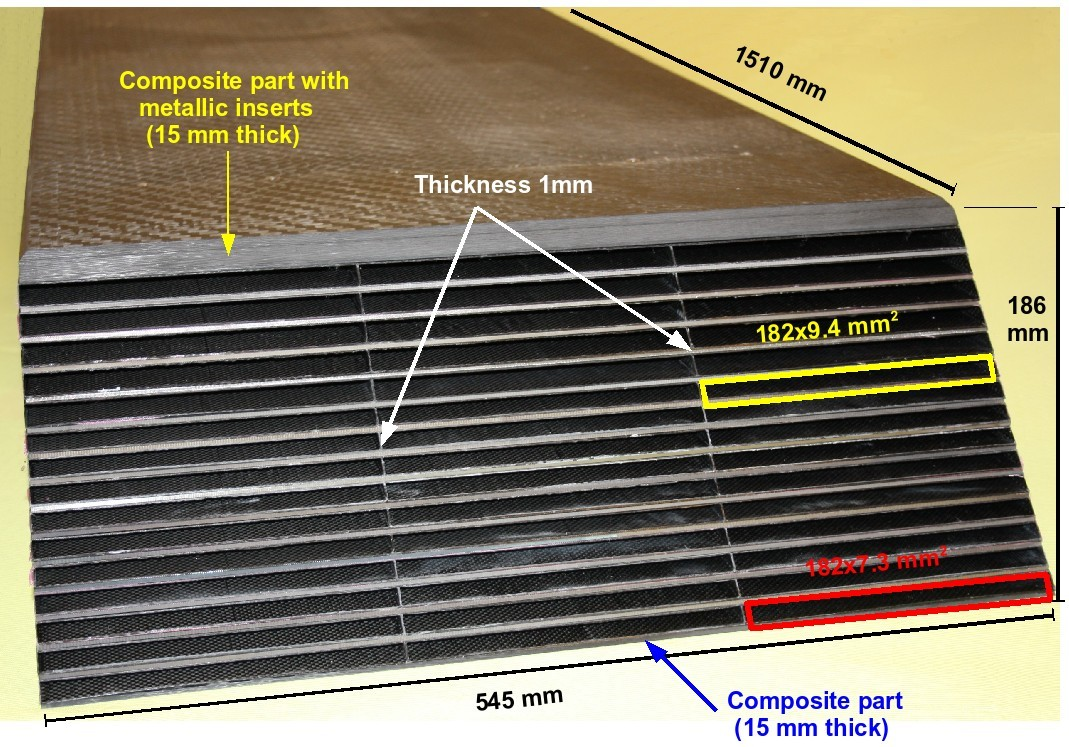
\includegraphics[width=5cm]{eudetecl.png}};
\node [rectangle,fill=white,opacity=1] at (-1,-1.) {EUDET ECAL concept};
\end{tikzpicture}
\column{6cm}
SiD design:\\
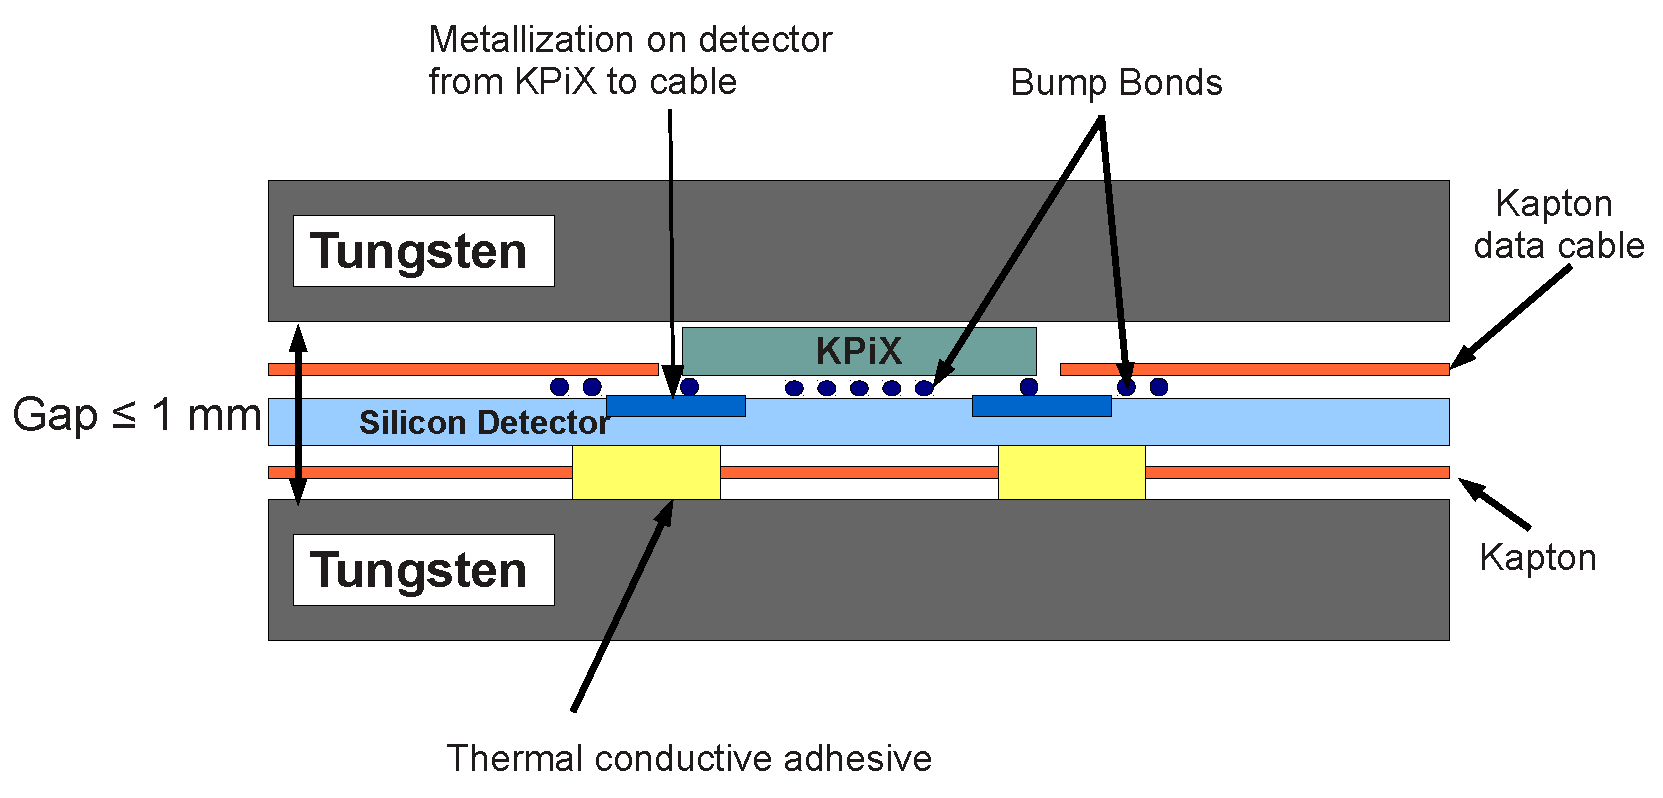
\includegraphics[width=6cm]{sid-ecal-drawing.pdf}
\end{columns}
\end{frame}
\begin{frame}
\frametitle{HCAL}
\begin{center}
\begin{tabular}{cc}
\toprule
Absorber (Barrel/Endcap) & Tungsten / Steel \\
\midrule
Sampling layers (B/E) & $75\times10$mm/ $60\times20$mm\\
\midrule
Cell size ($\textrm{mm}^2$) & $30\times30$ (SiPM), $10\times10$ (RPC)\\
\midrule
$\lambda_{\textrm{I}}$ & 7.5\\
\bottomrule
\end{tabular}
\end{center}
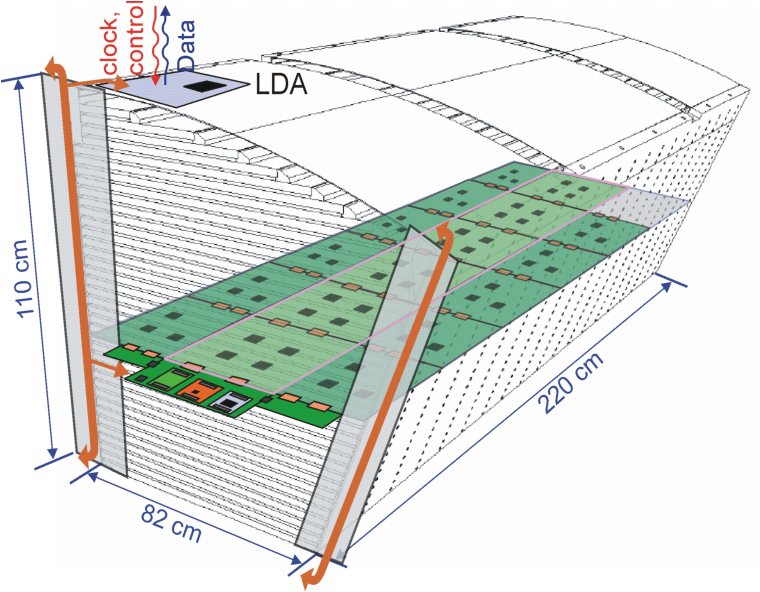
\includegraphics[width=6cm]{Fig817a.pdf}
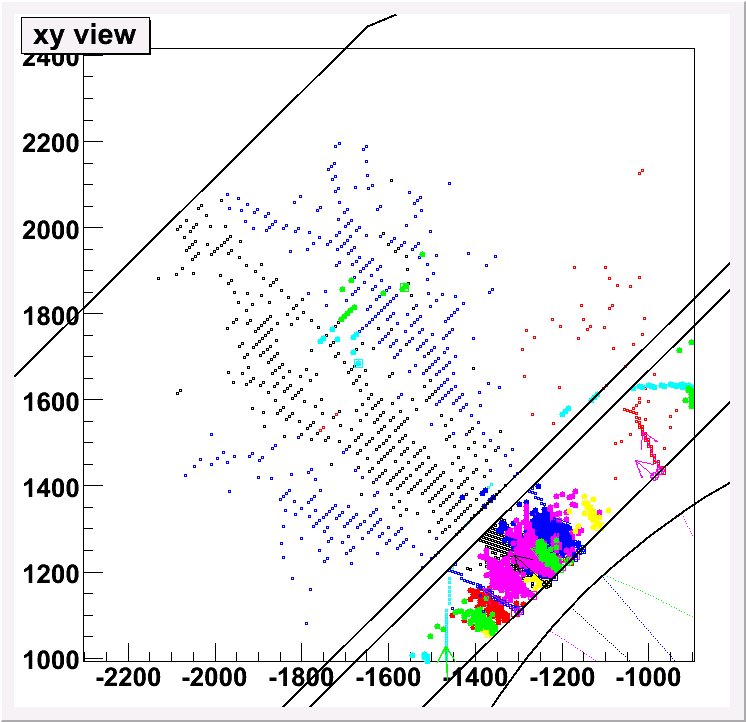
\includegraphics[width=5cm]{hcalzoom.png}
\end{frame}
\begin{frame}
\frametitle{CALICE beam tests for W-HCAL}
\alert{Validation of GEANT4 simulation for hadronic showers in tungsten}\\
\begin{columns}[c]
\column{5cm}
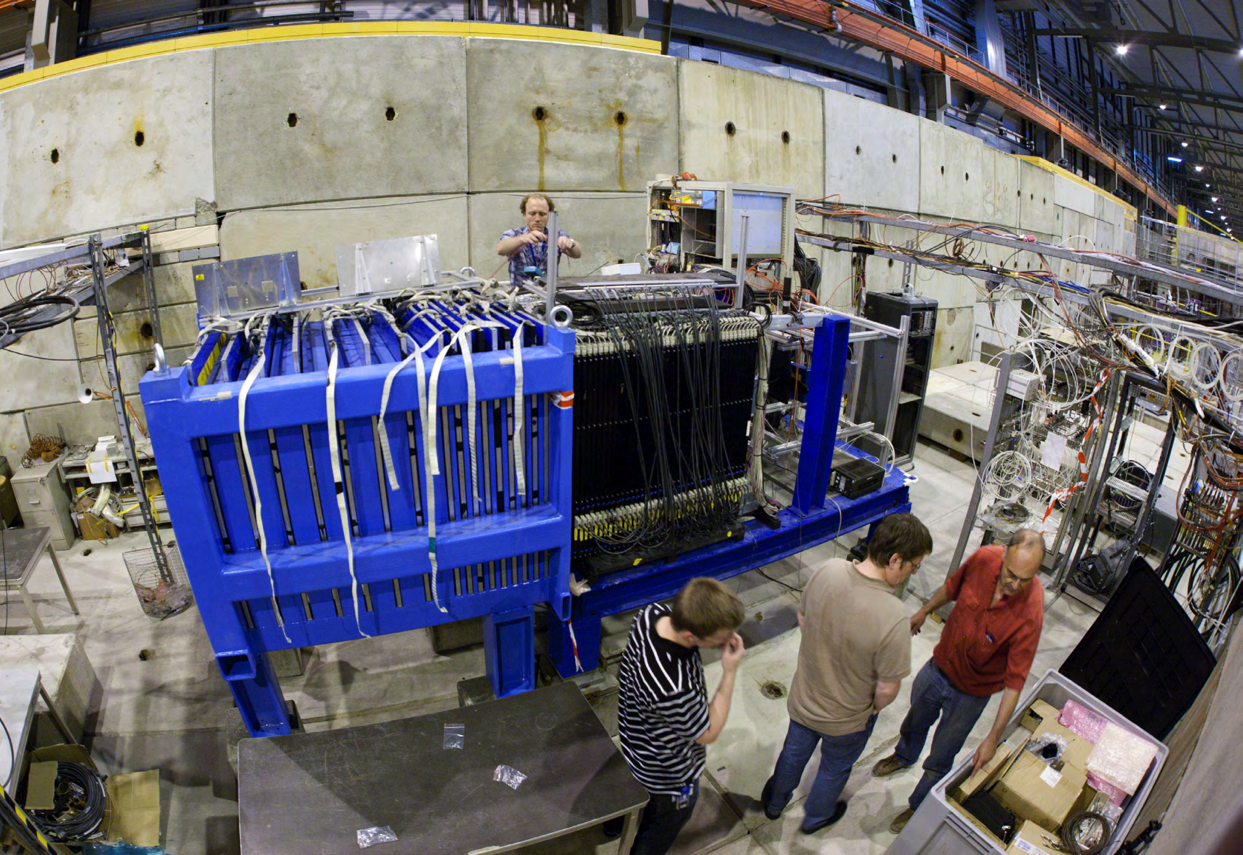
\includegraphics[width=5cm]{whcal_model.png}
\column{4cm}
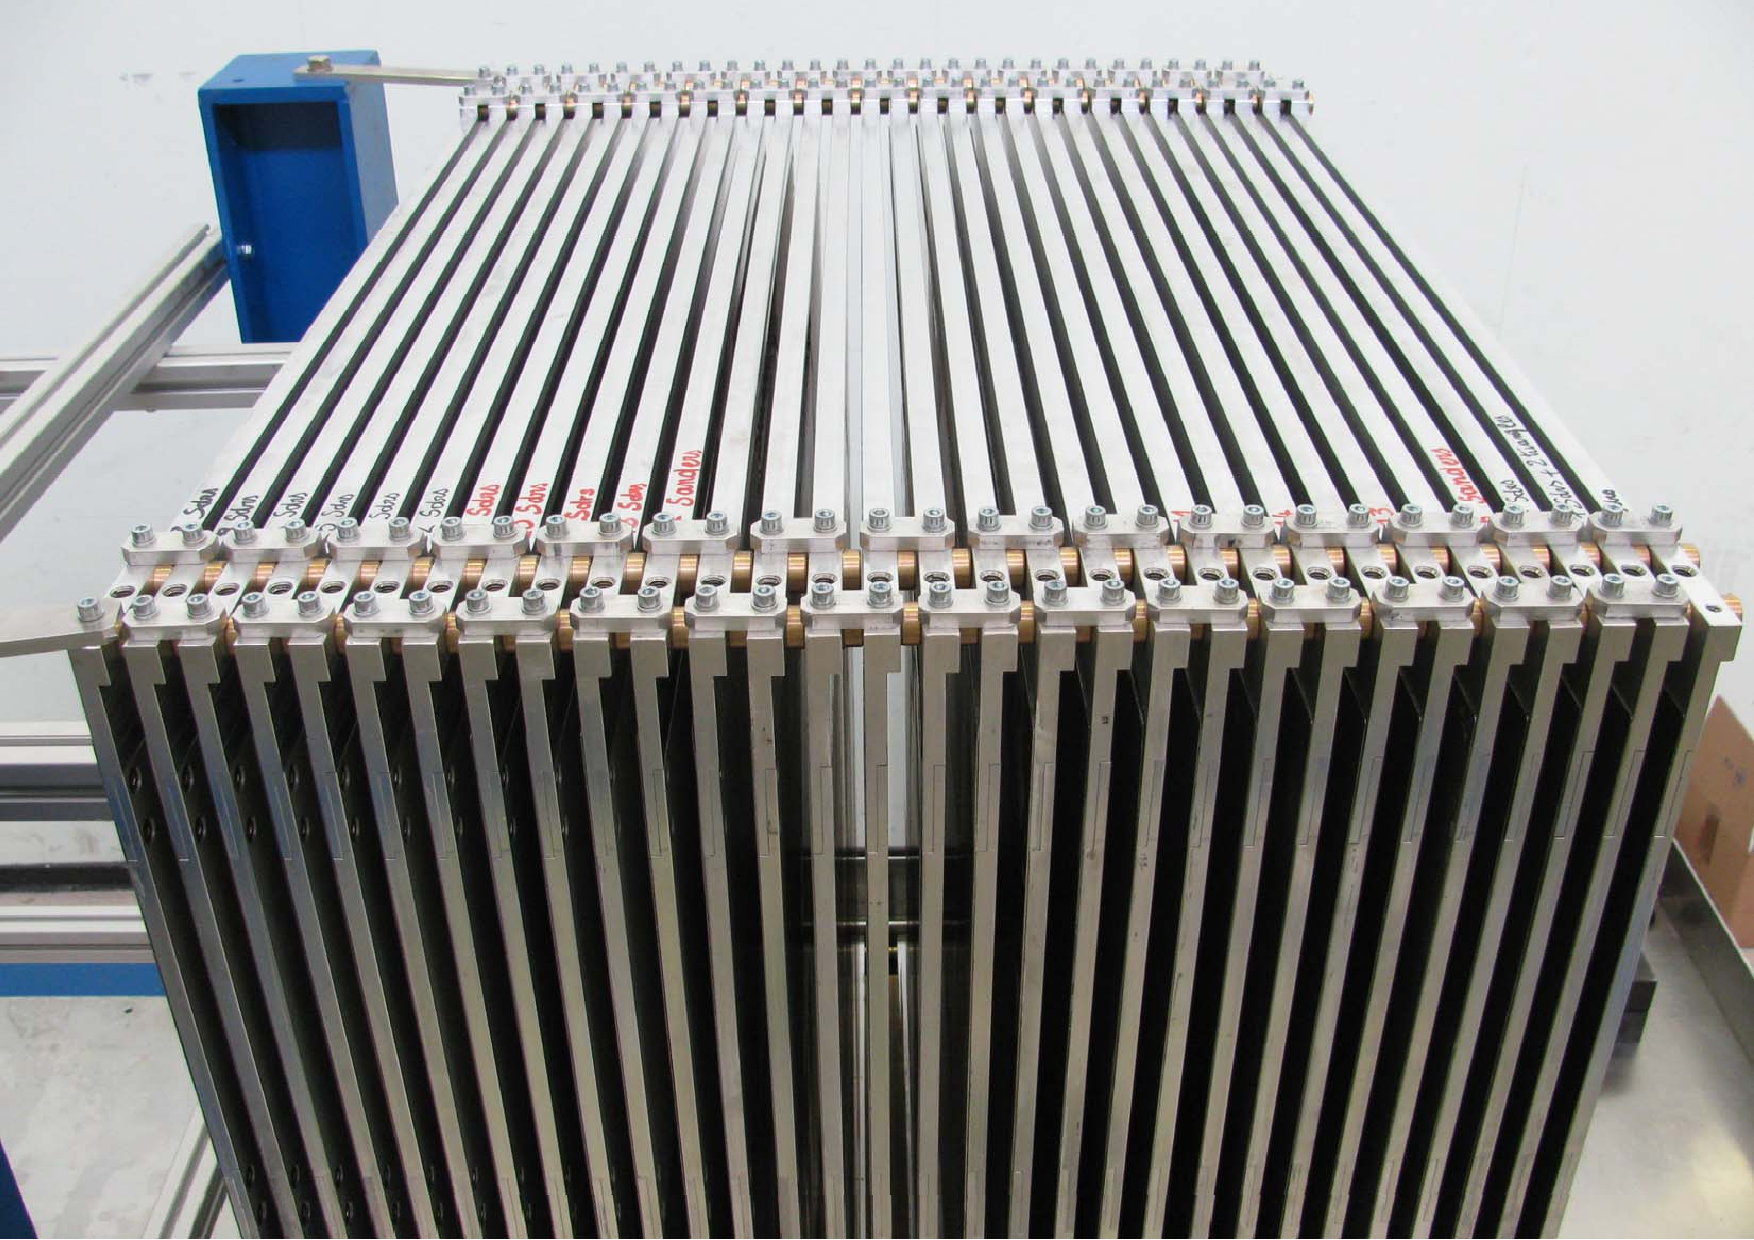
\includegraphics[width=4cm]{Fig820b.pdf}
\column{3cm}
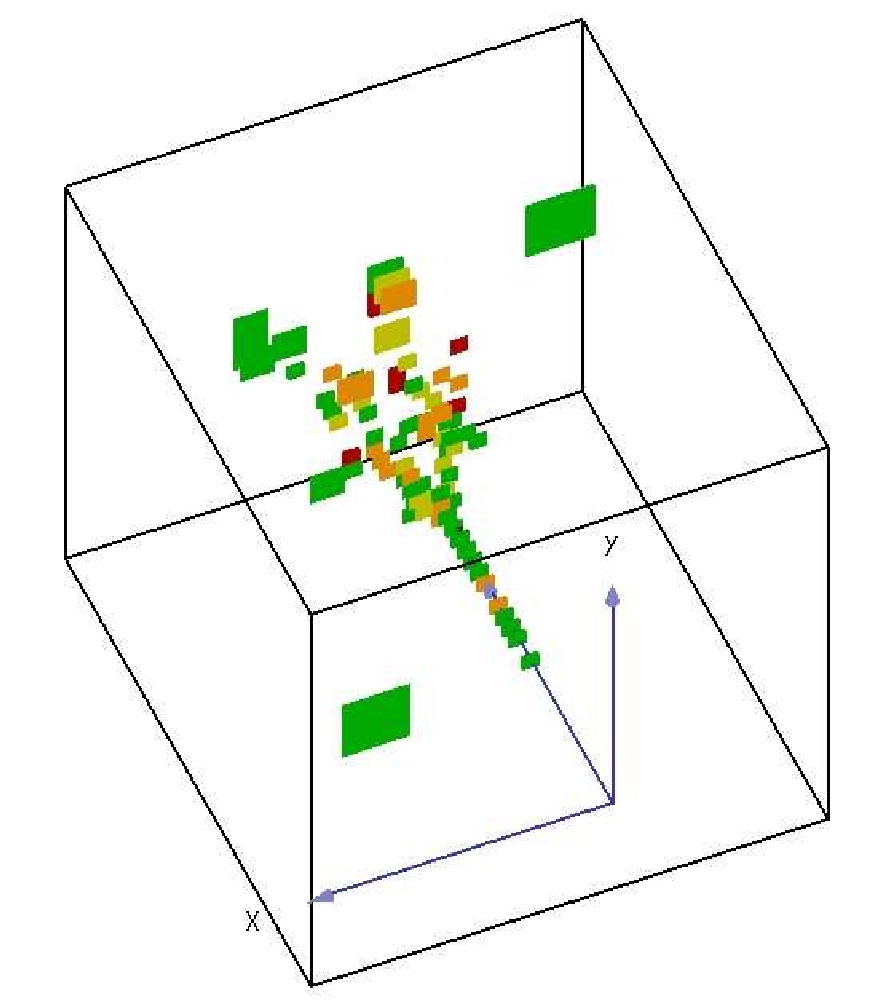
\includegraphics[width=3cm]{Fig820c.pdf}
\end{columns}
\begin{columns}[c]
\column{5cm}
Test beam period in 2010-2011\\
Analysis ongoing
\column{4cm}
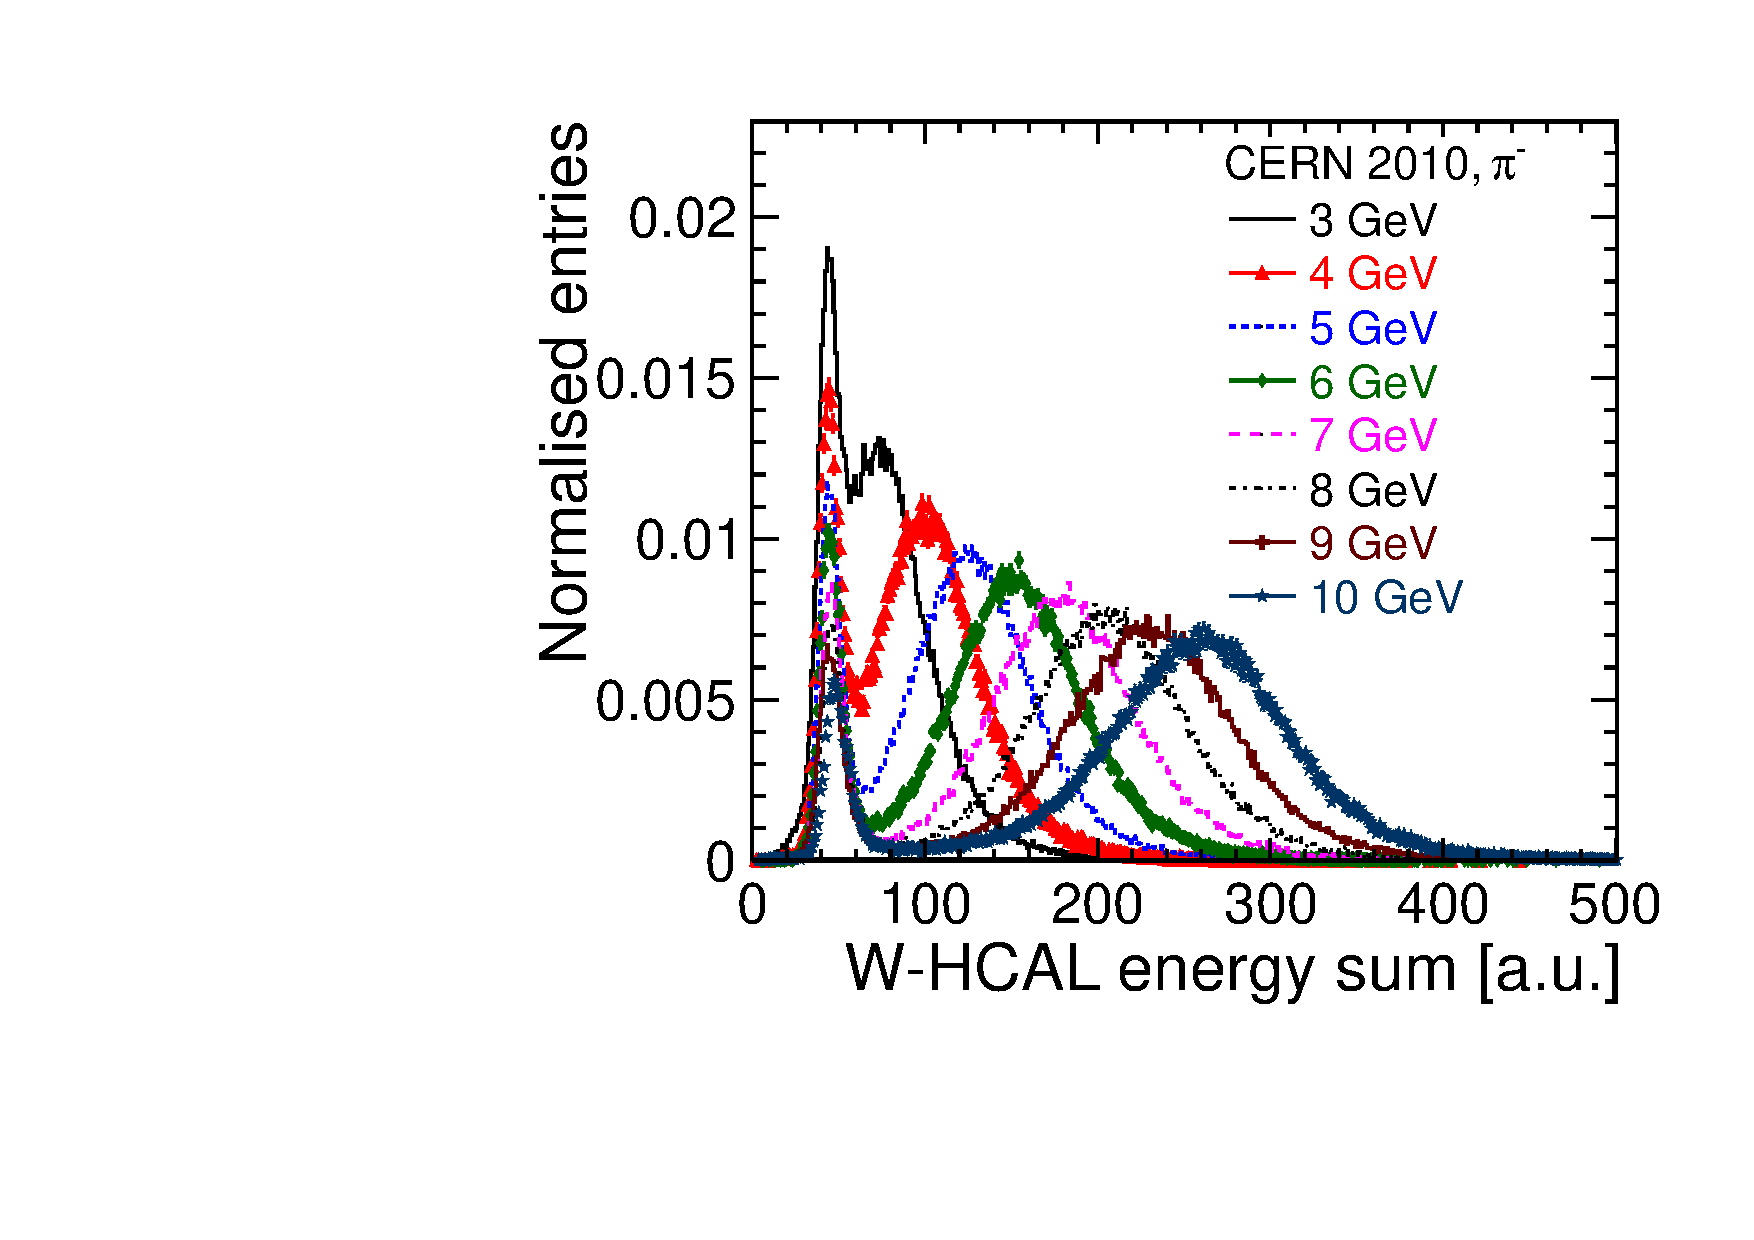
\includegraphics[width=4cm]{Fig821.pdf}
\column{4cm}
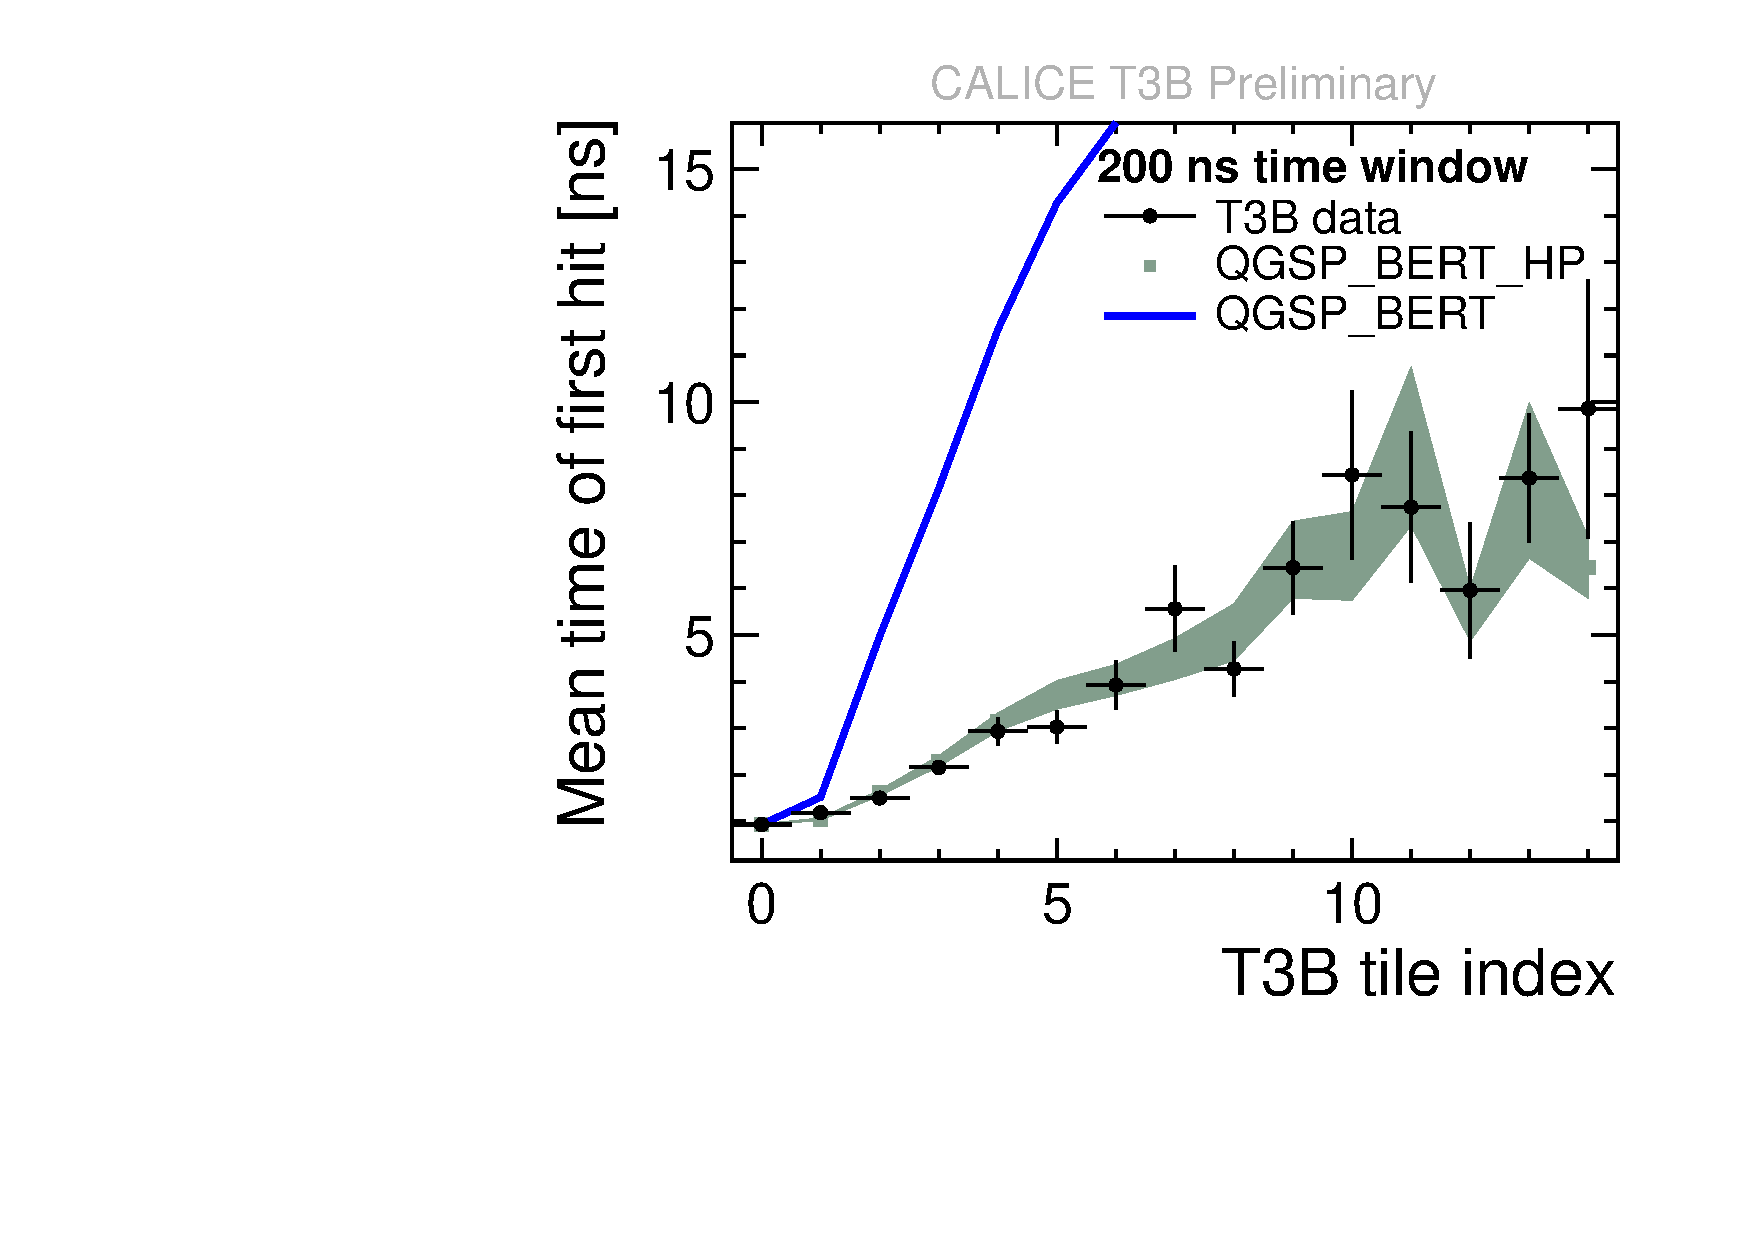
\includegraphics[width=4cm]{Fig824.pdf}
\end{columns}
\end{frame}

\section[Bkg treatment]{Suppression of beam-induced background}
\begin{frame}
\frametitle{Background properties}
Main problematic background: $\gamma\gamma\to\textrm{hadrons}$
\begin{columns}[c]
\column{6cm}
\centering
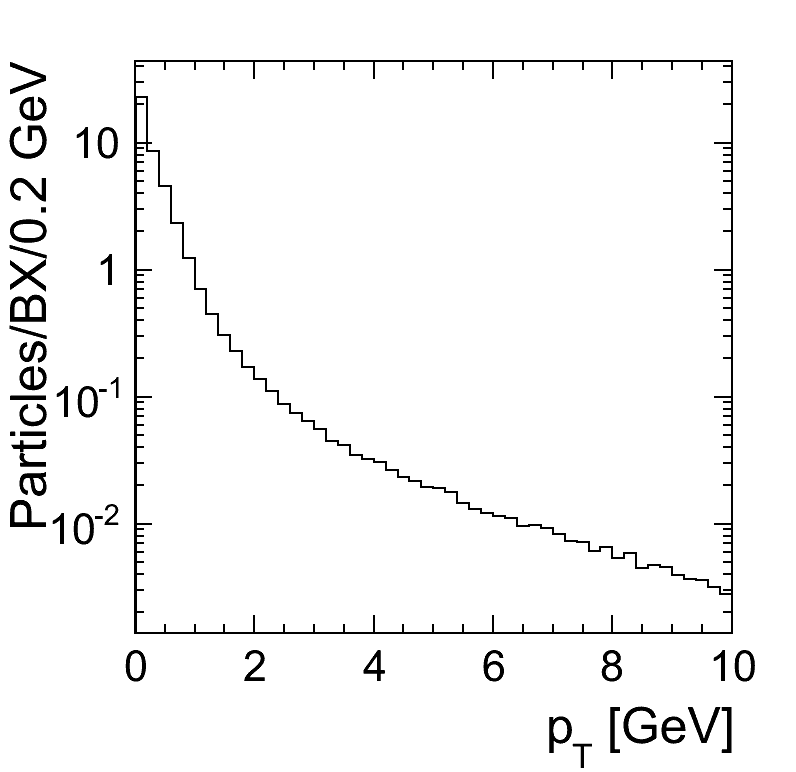
\includegraphics[width=4cm]{../SIDWorkshop/ggPT}\\
$\theta>8^\circ$
\column{6cm}
Entire bunch train (312BX):
\begin{itemize}
  \item 5000 tracks $\to$ total track momentum: \alert{7.3TeV}
  \item Total calorimetric energy (ECAL+HCAL): \alert{19TeV}
\end{itemize}
Mostly low $p_{\textrm{T}}$
\end{columns}
\end{frame}
\begin{frame}
\frametitle{Timing cuts}
\begin{columns}[c]
\column{5cm}
\centering
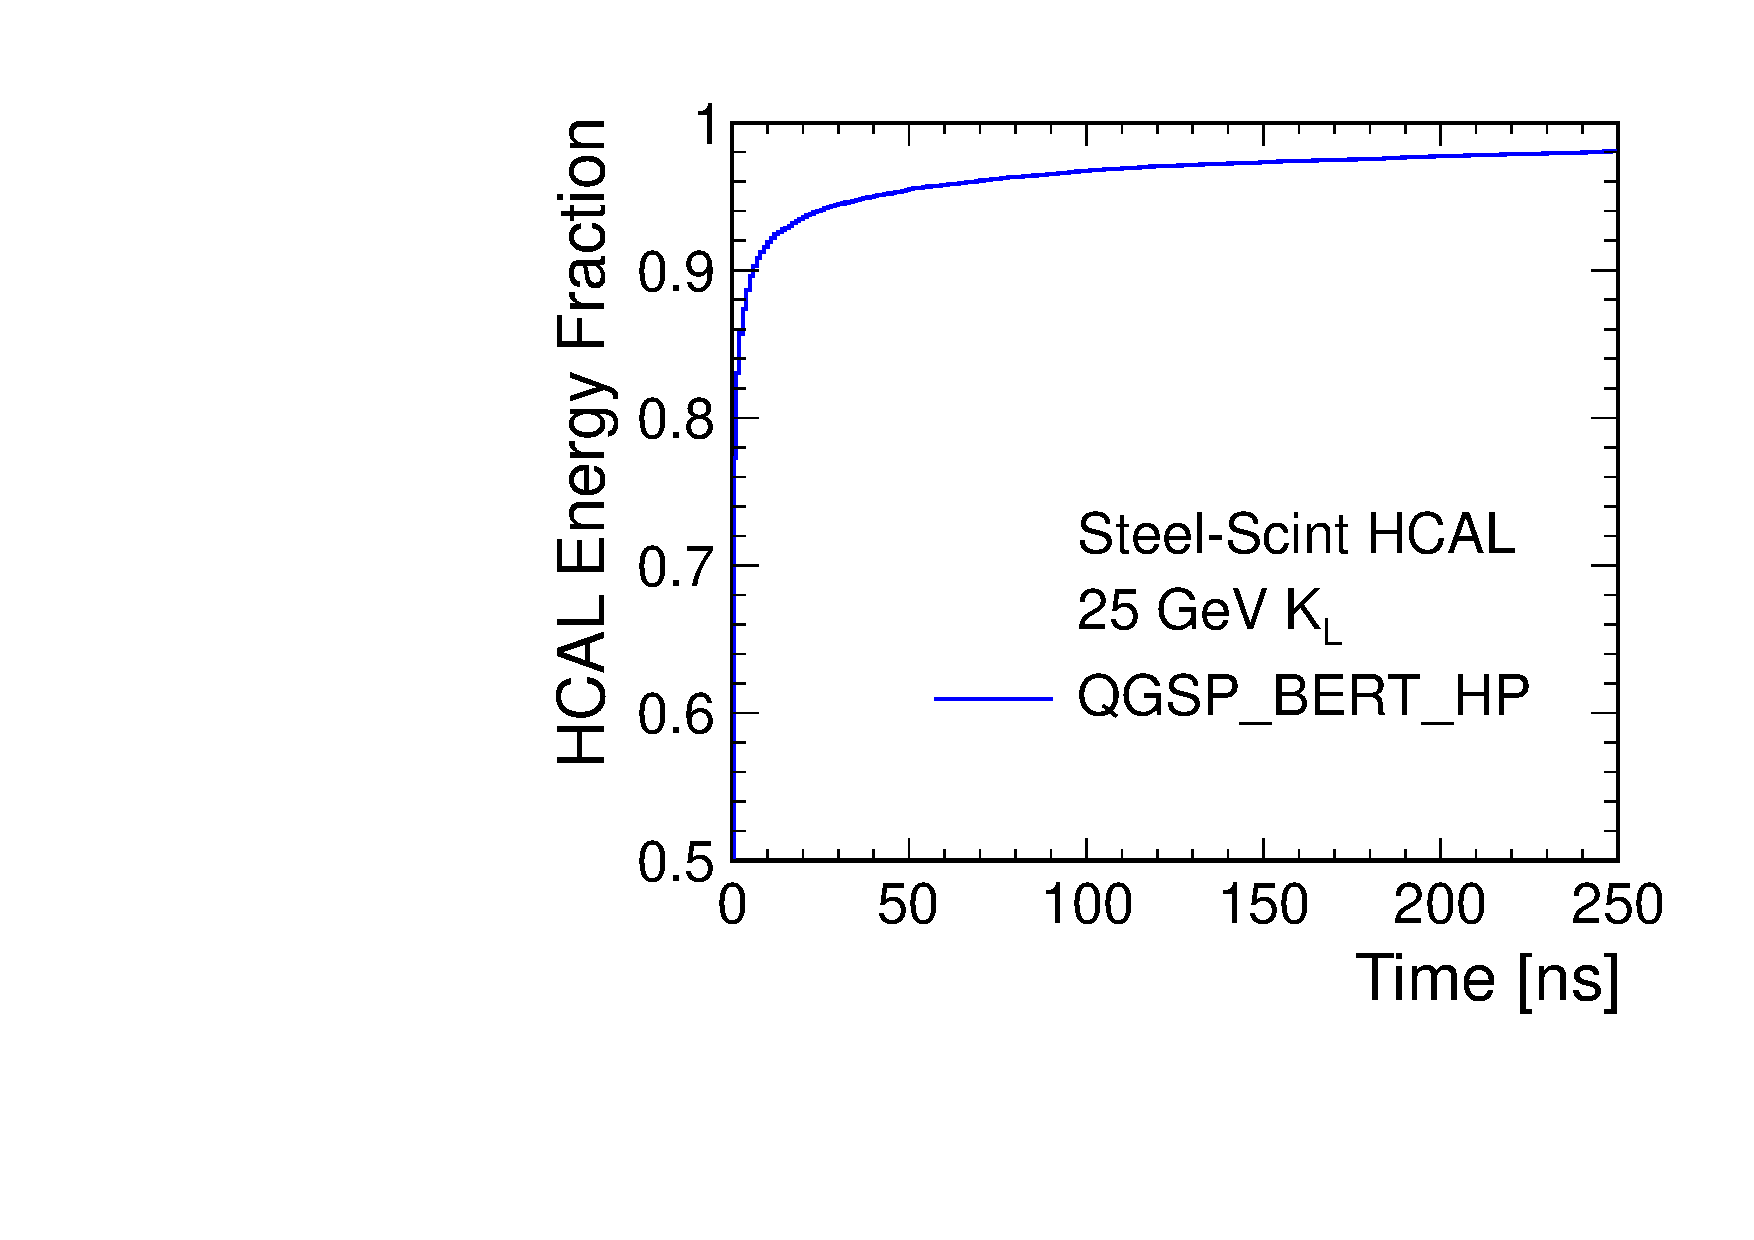
\includegraphics[width=5cm]{../SIDWorkshop/hcalTimingSteel.pdf}
\column{5cm}
\centering
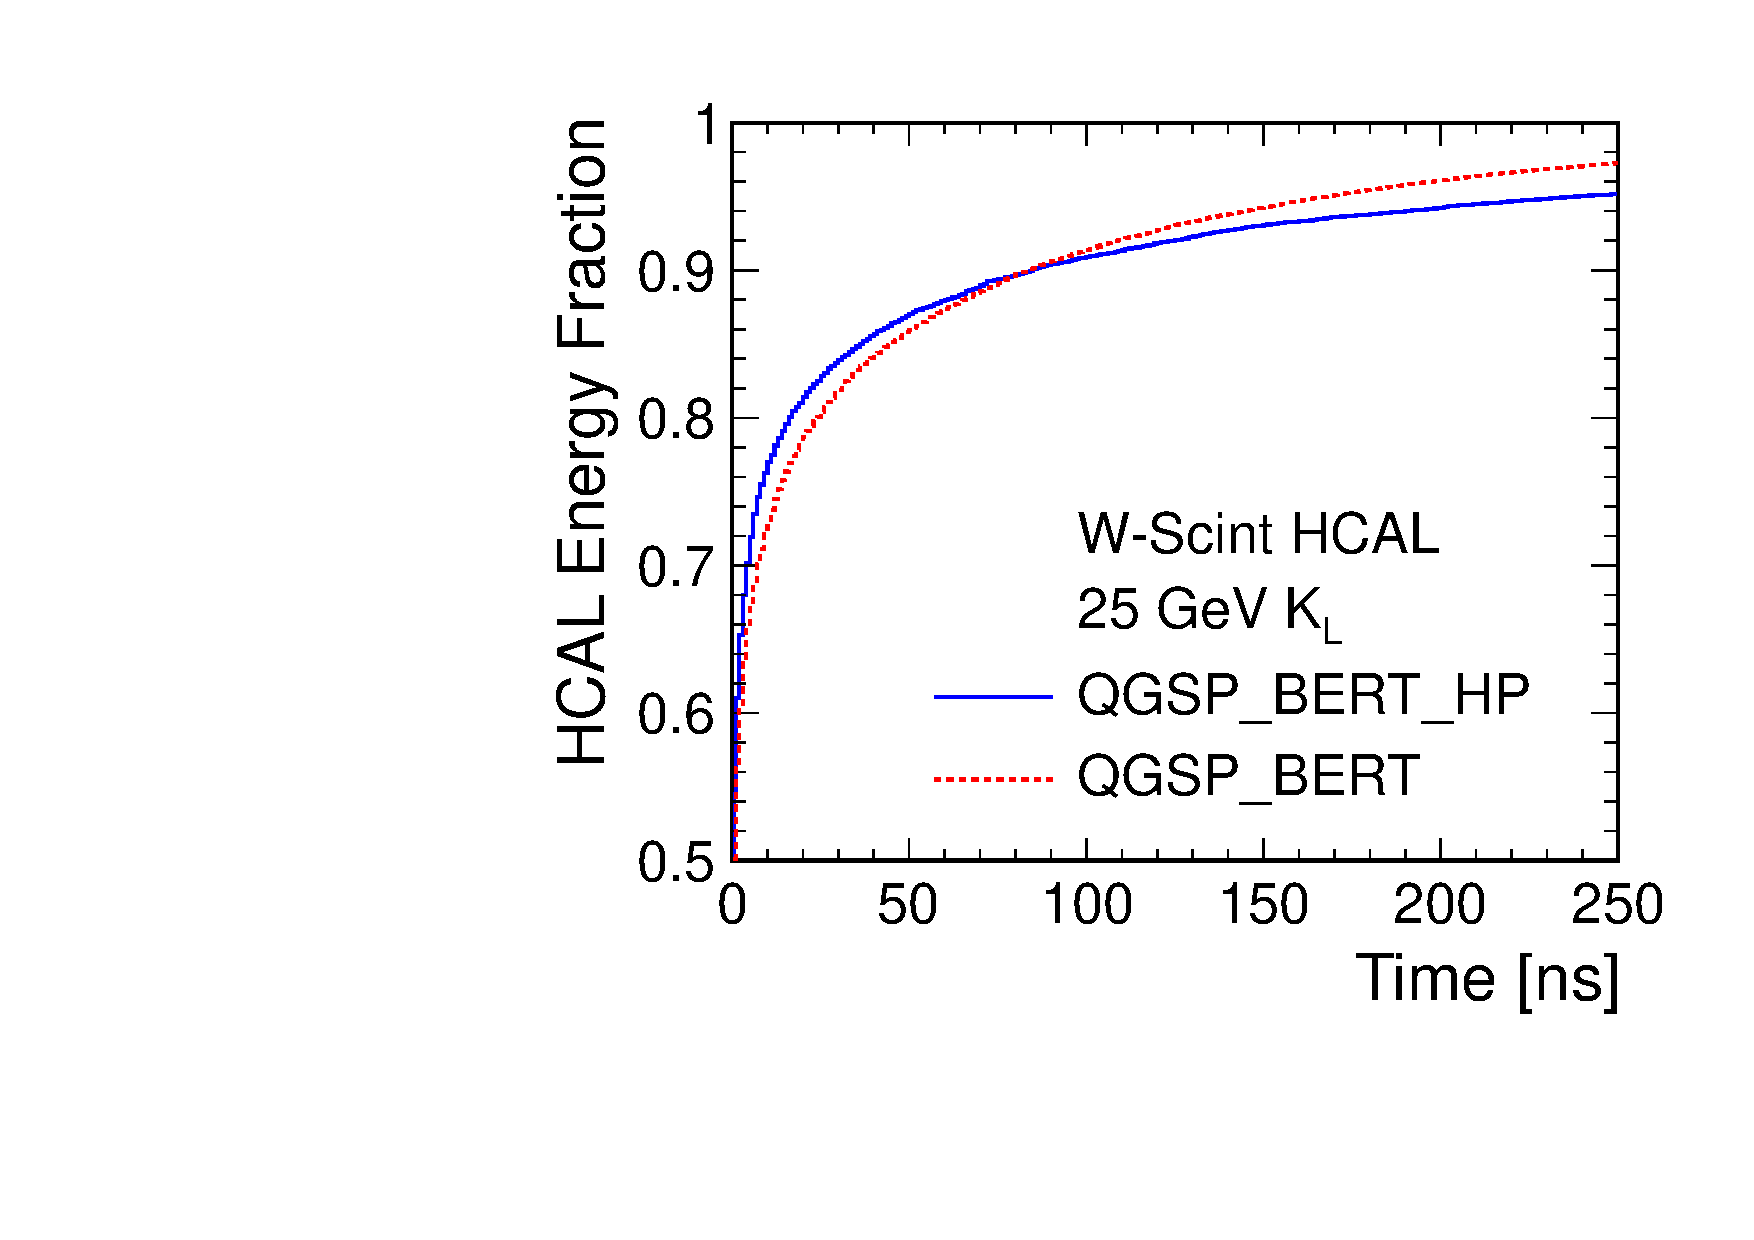
\includegraphics[width=5cm]{../SIDWorkshop/hcalTimingTungsten.pdf}
\end{columns}
\begin{center}
\begin{tabular}{lrr}
Subdetector &Reco. window &hit resolution\\
ECAL &10 ns &1 ns\\
HCAL Endcaps &10 ns &1 ns\\
HCAL Barrel &100 ns &1 ns\\
Silicon Detectors &10 ns &$10/\sqrt{12}$ ns\\
TPC & entire bunch train & n/a
\end{tabular}
\end{center}
Additionnal timing cuts applied on reconstructed particles.
\end{frame}
\begin{frame}
\frametitle{Jet finder}
$\Pep\Pem\to\PSq_R\PaSq_R\to\Pquark\APquark\PSgxz_1 \PSgxz_1$: 2 jets $+$
missing energy\\ ~\\
\begin{columns}[c]
\column{6cm}
Durham $k_{\textrm{T}}$ \`a la LEP:\\
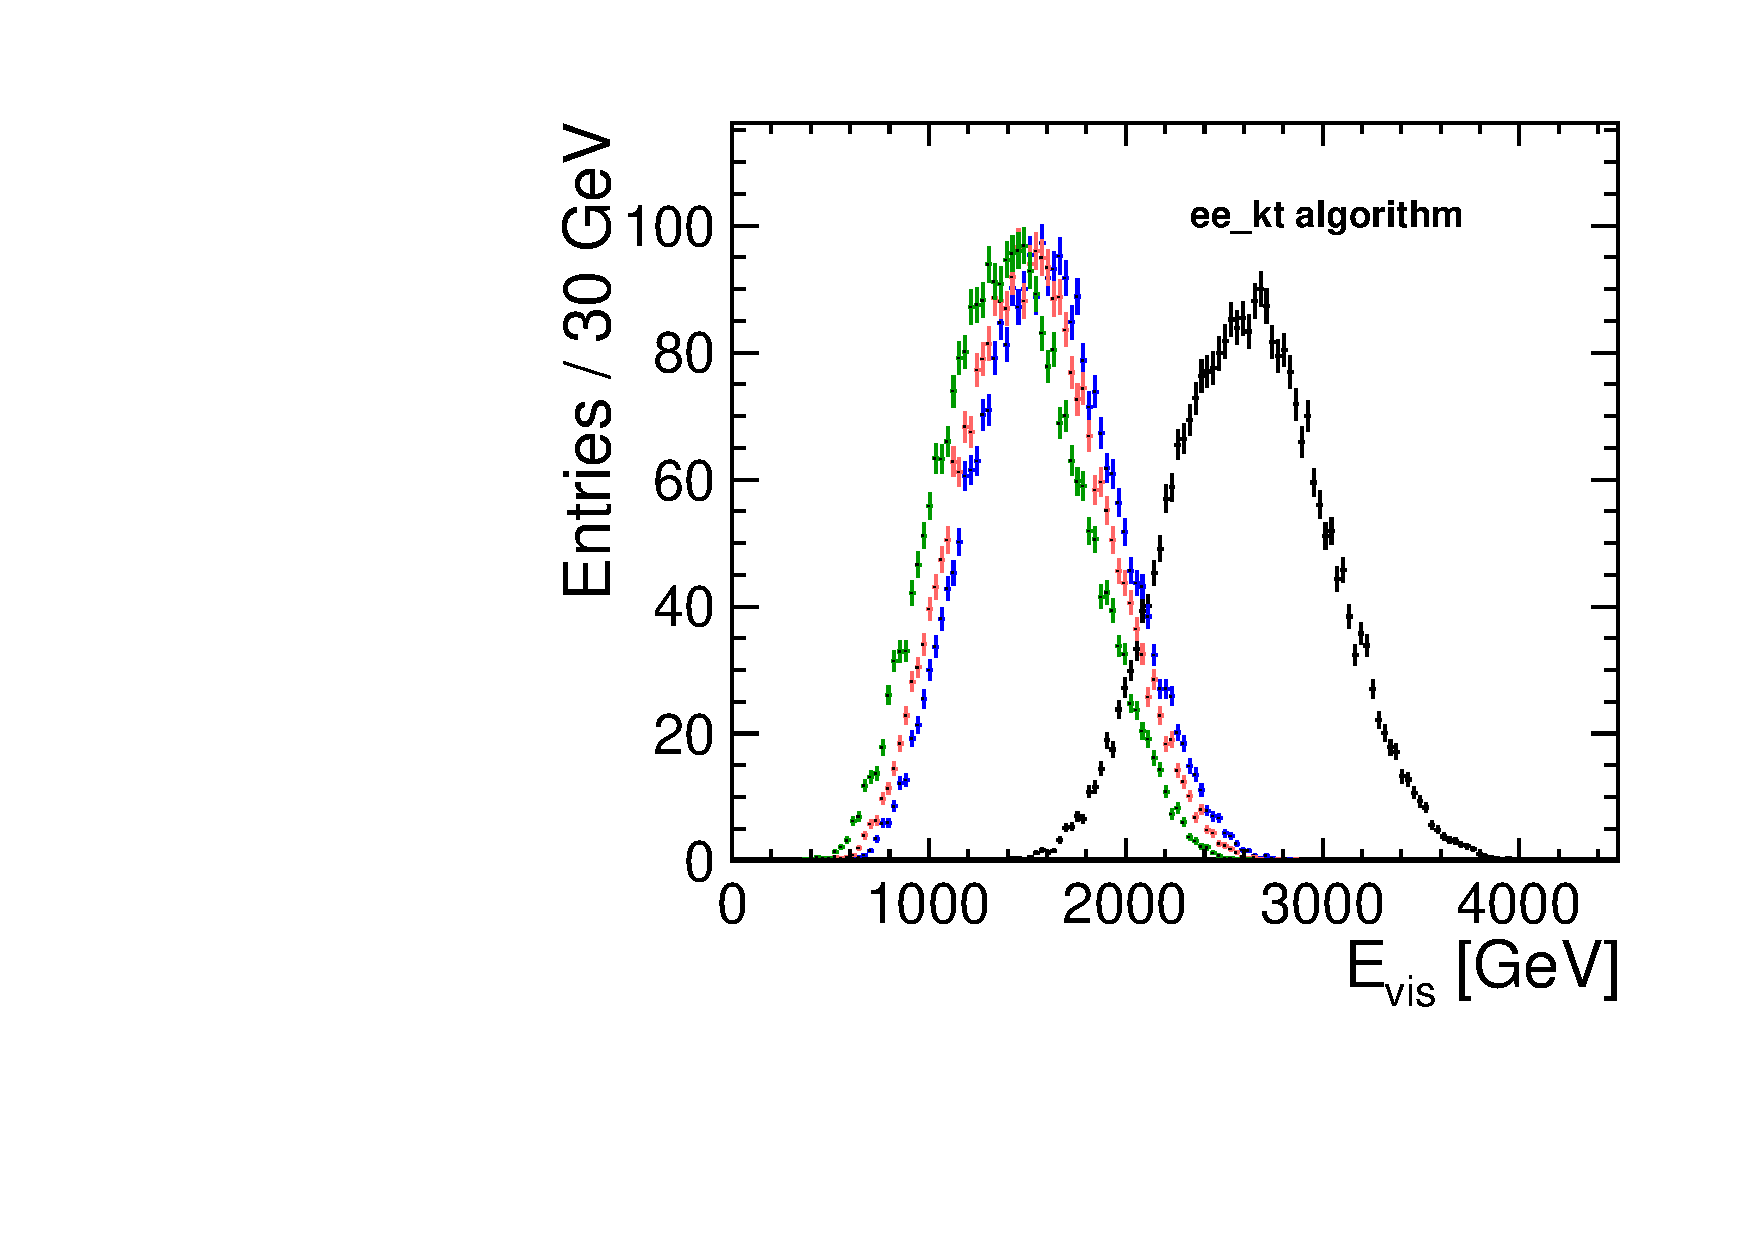
\includegraphics[width=6cm]{../SIDWorkshop/JetFinding_compare_E_vis__FJ_ee_kt_algorithm_ExclusiveNJets_2.pdf}\\
\column{6cm}
Hadron collider $k_{\textrm{T}}$:\\
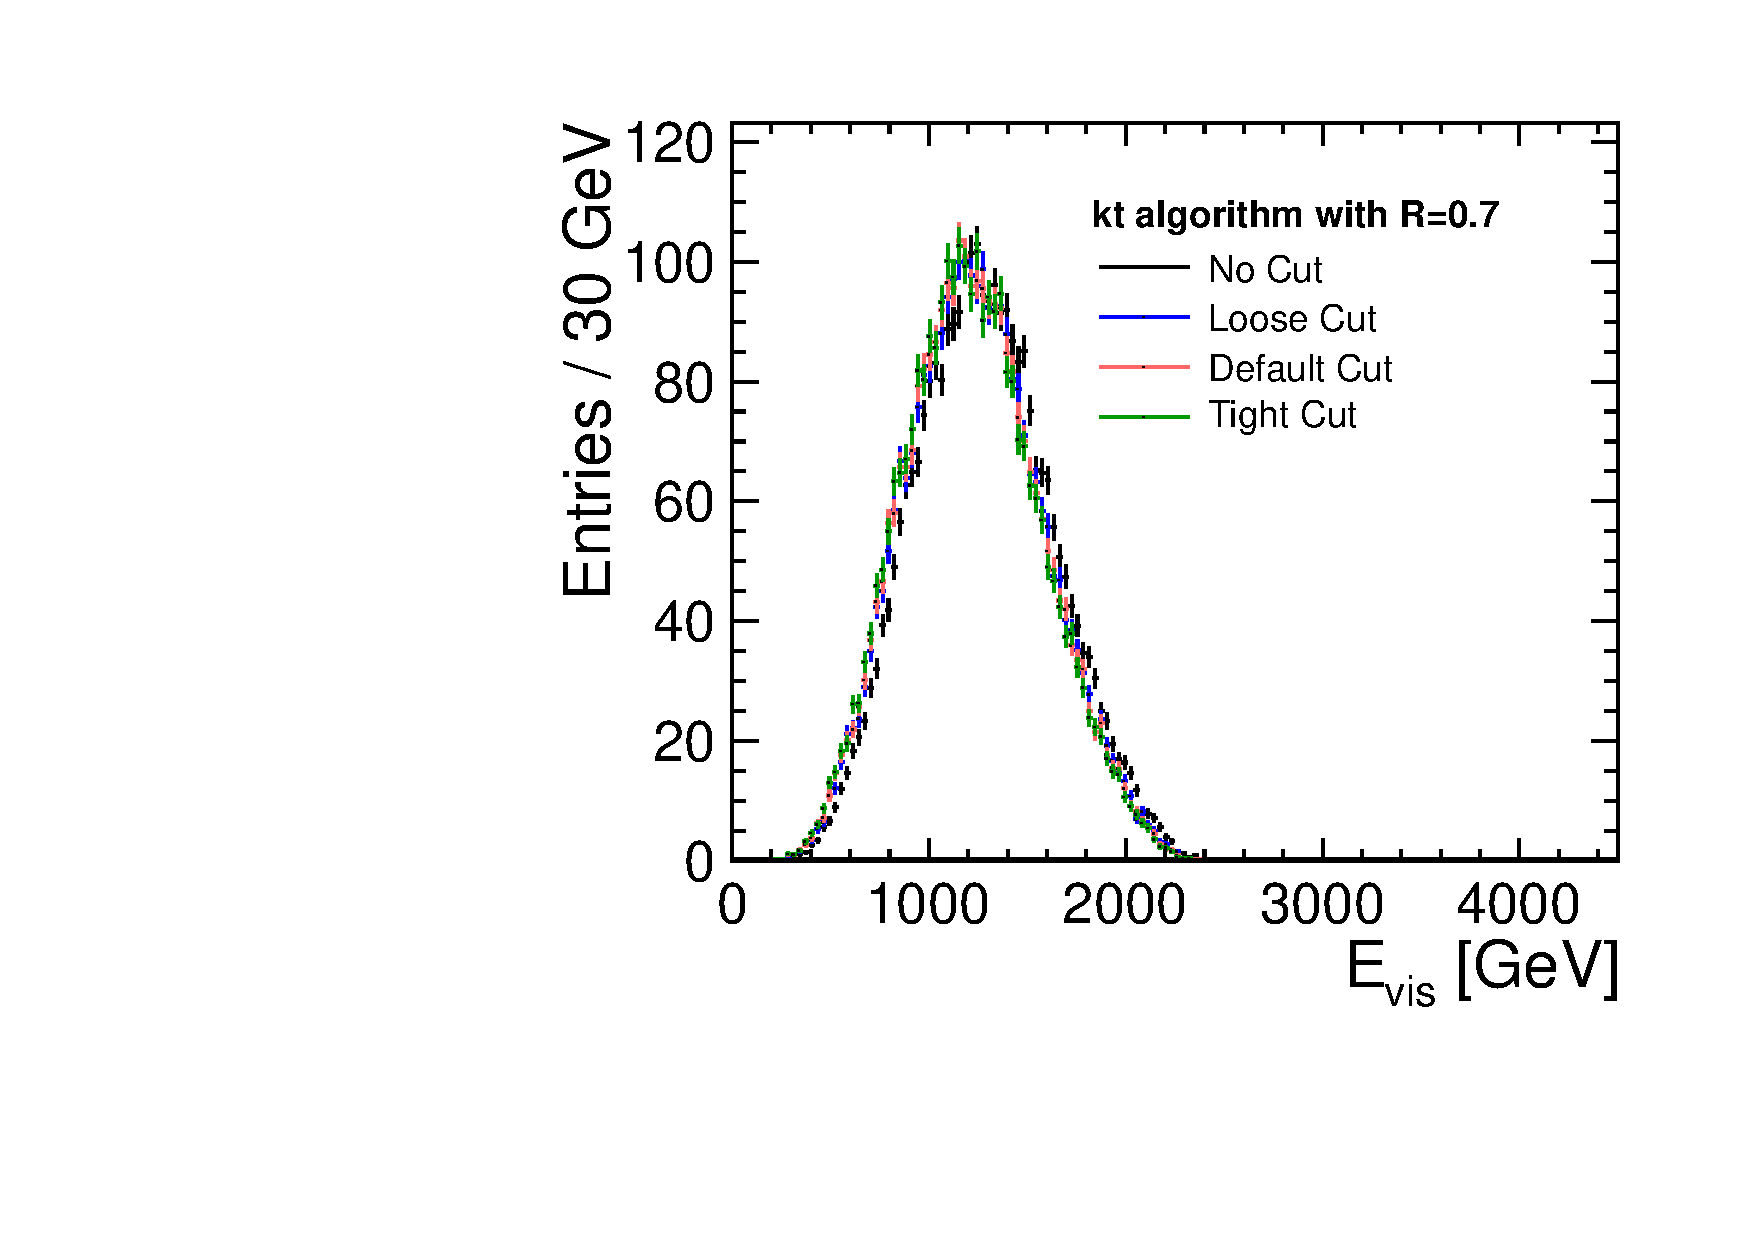
\includegraphics[width=6cm]{../SIDWorkshop/JetFinding_compare_E_vis__FJ_kt_algorithm_0_7_ExclusiveNJets_2.pdf}\\
\end{columns}
\begin{columns}
\column{6cm}
{\scriptsize
\begin{itemize}
  \item All particle clustered
  \item Timing cuts effective
\end{itemize}
}
\column{6cm}
{\scriptsize
\begin{itemize}
  \item Much of Bkg clustered with beam axis
  \item Timing cuts do less work
  \item Impact depends on event topology
\end{itemize}
}
\end{columns}
\end{frame}
\begin{frame}
\frametitle{Background suppression}
E.g. $\Pep\Pem\to\PHp\PHm\to\Ptop\APbottom\Pbottom\APtop$:
\begin{columns}[c]
\column{6cm}
\centering
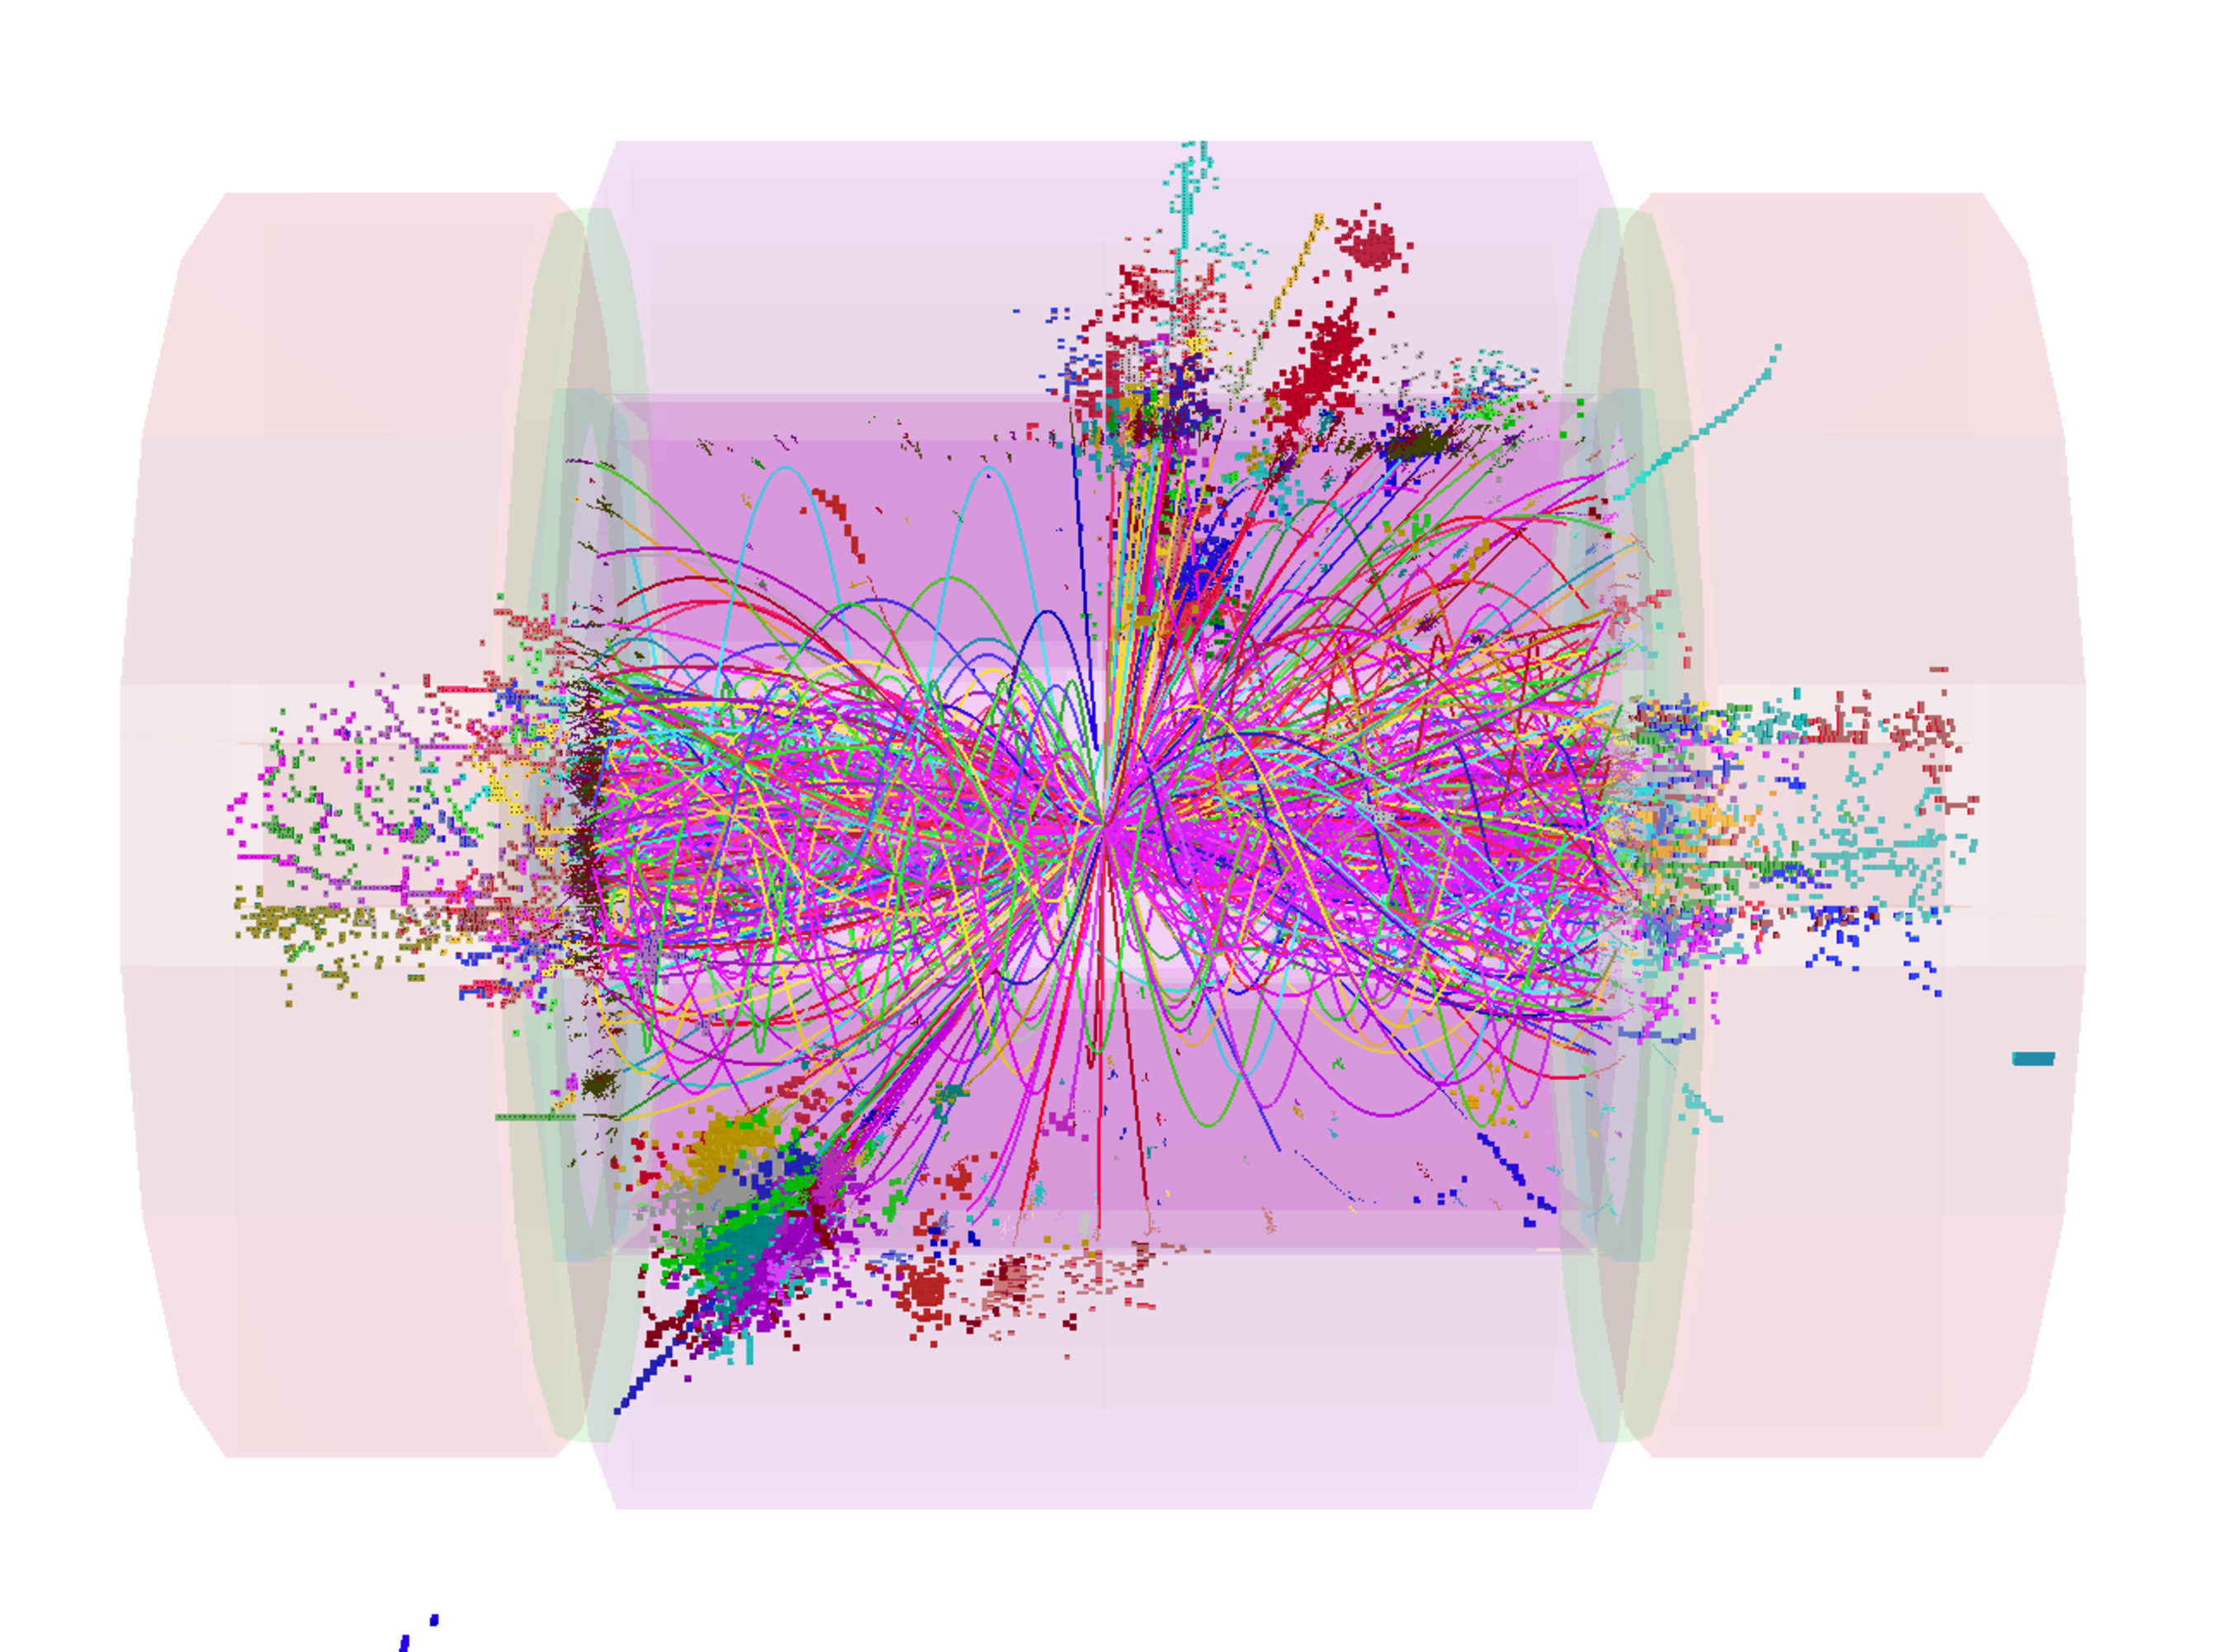
\includegraphics[width=6cm]{../SIDWorkshop/HH2.pdf}
\column{6cm}
\centering
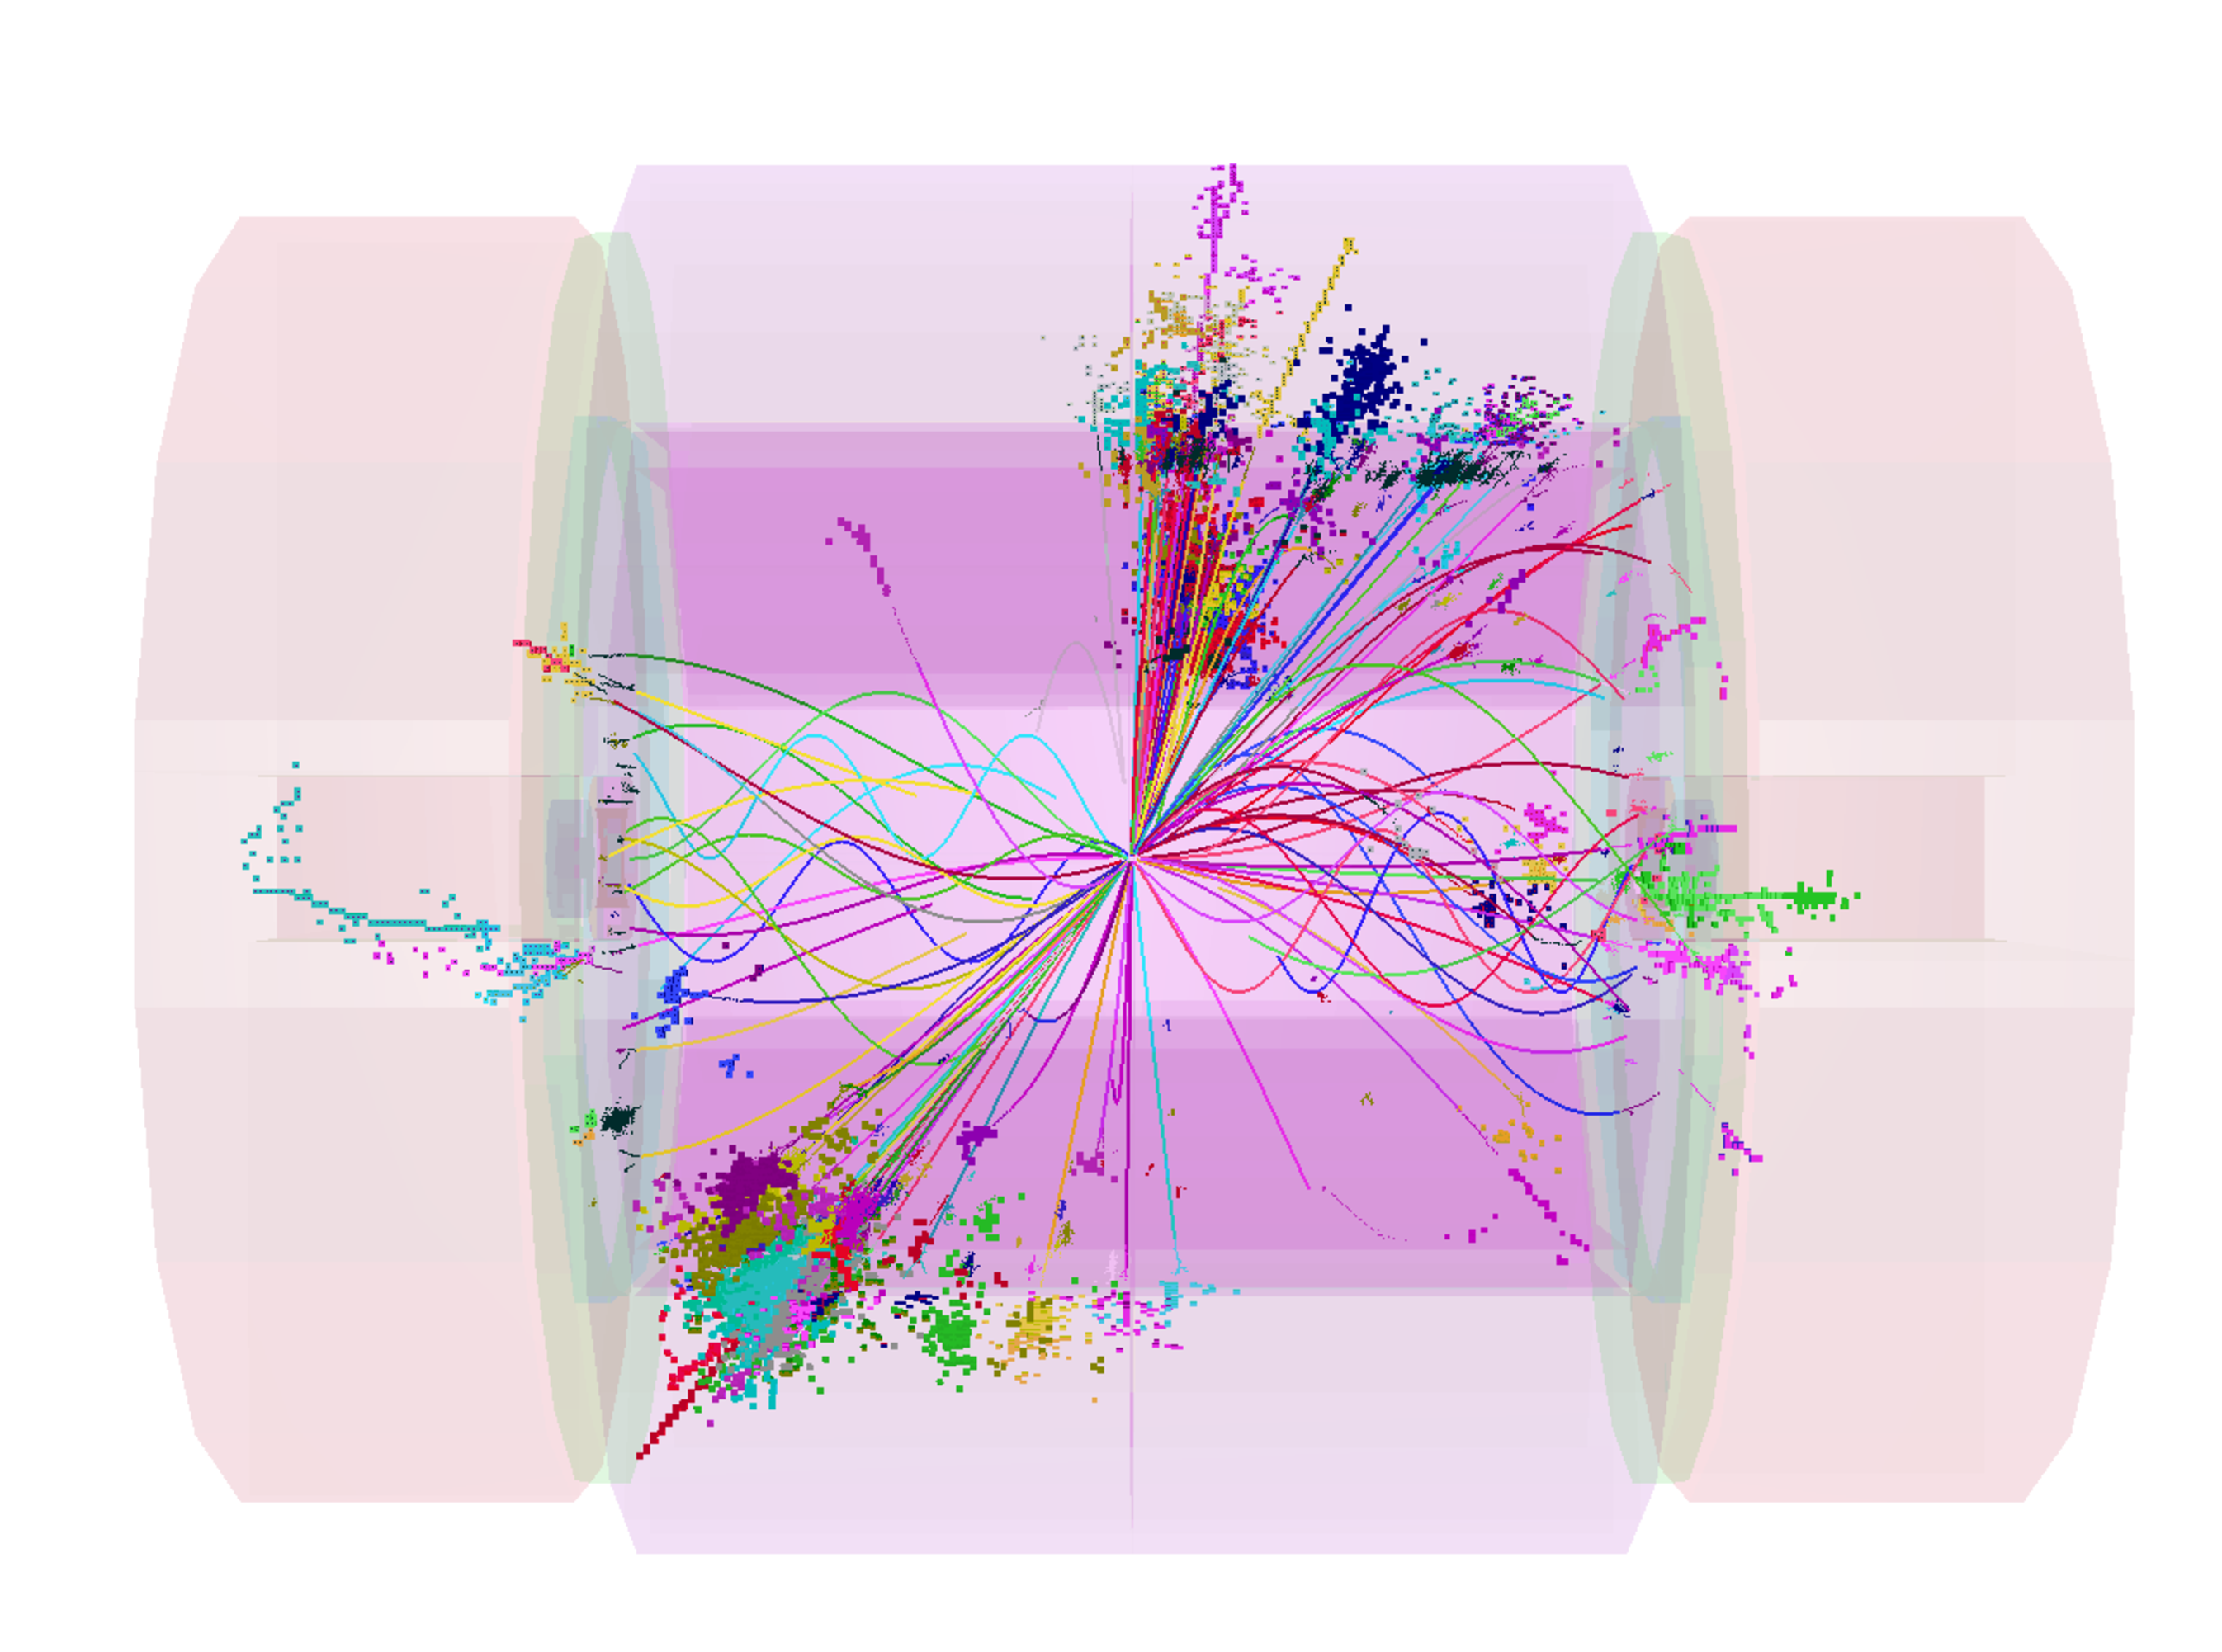
\includegraphics[width=6cm]{../SIDWorkshop/HH2tight.pdf}
\end{columns}
\begin{columns}[c]
\column{6cm}
\centering
No cuts:\\ \alert{$\sim1.2\textrm{TeV}$}\\
{\color{blue}{\scriptsize 10ns window}}
\column{6cm}
\centering
Tight timing cuts:\\ \alert{$\sim100\textrm{GeV}$}
\end{columns}
~\\
\alert{Using timing cuts and jet finding removes most of the background}
\end{frame}

\section{Benchmarking the detectors}
\begin{frame}
 \frametitle{Benchmark channels}
The benchmark channels used to assess detector performance:
\begin{itemize}
\item $\Pep\Pem \to \Ph \Pgne \Pagne, \Ph \to \mu^+\mu^-, \Ph \to
\Pbottom\APbottom$ (CLIC\_SID),
\item  $\Pep\Pem \to \PHp \PHm\to \Ptop\APbottom\APtop\Pbottom$(CLIC\_ILD),\\
$\Pep\Pem \to \PHz \PA\to\Pbottom\APbottom\Pbottom\APbottom$ (CLIC\_ILD),
\item $\Pep\Pem \to \PSq_R \PaSq_R\to\Pquark\APquark\PSgxz_1\PSgxz_1$
(CLIC\_ILD),
\item $\Pep\Pem \to \PSl \PaSl \,(\ell = \Pe,\Pgm,\Pgne)$ (CLIC\_ILD), 
\item $\Pep\Pem \to \PSgxpm_1 \PSgxmp_1\to\PWp\PWm\PSgxz_1\PSgxz_1$
(CLIC\_SID),\\ $\Pep\Pem \to \PSgxz_2 \PSgxz_2\to \Ph\Ph\PSgxz_1\PSgxz_1$
(CLIC\_SID),
\item  $\Pep\Pem \to \Pqt \Paqt$ (500~GeV, CLIC\_ILD).
\end{itemize} 
\end{frame}
\begin{frame}
\frametitle{SM Higgs decays}
Flavour tagging ($\Ph\to\Pbottom\APbottom$):
\begin{columns}[c]
\column{4cm}
\centering
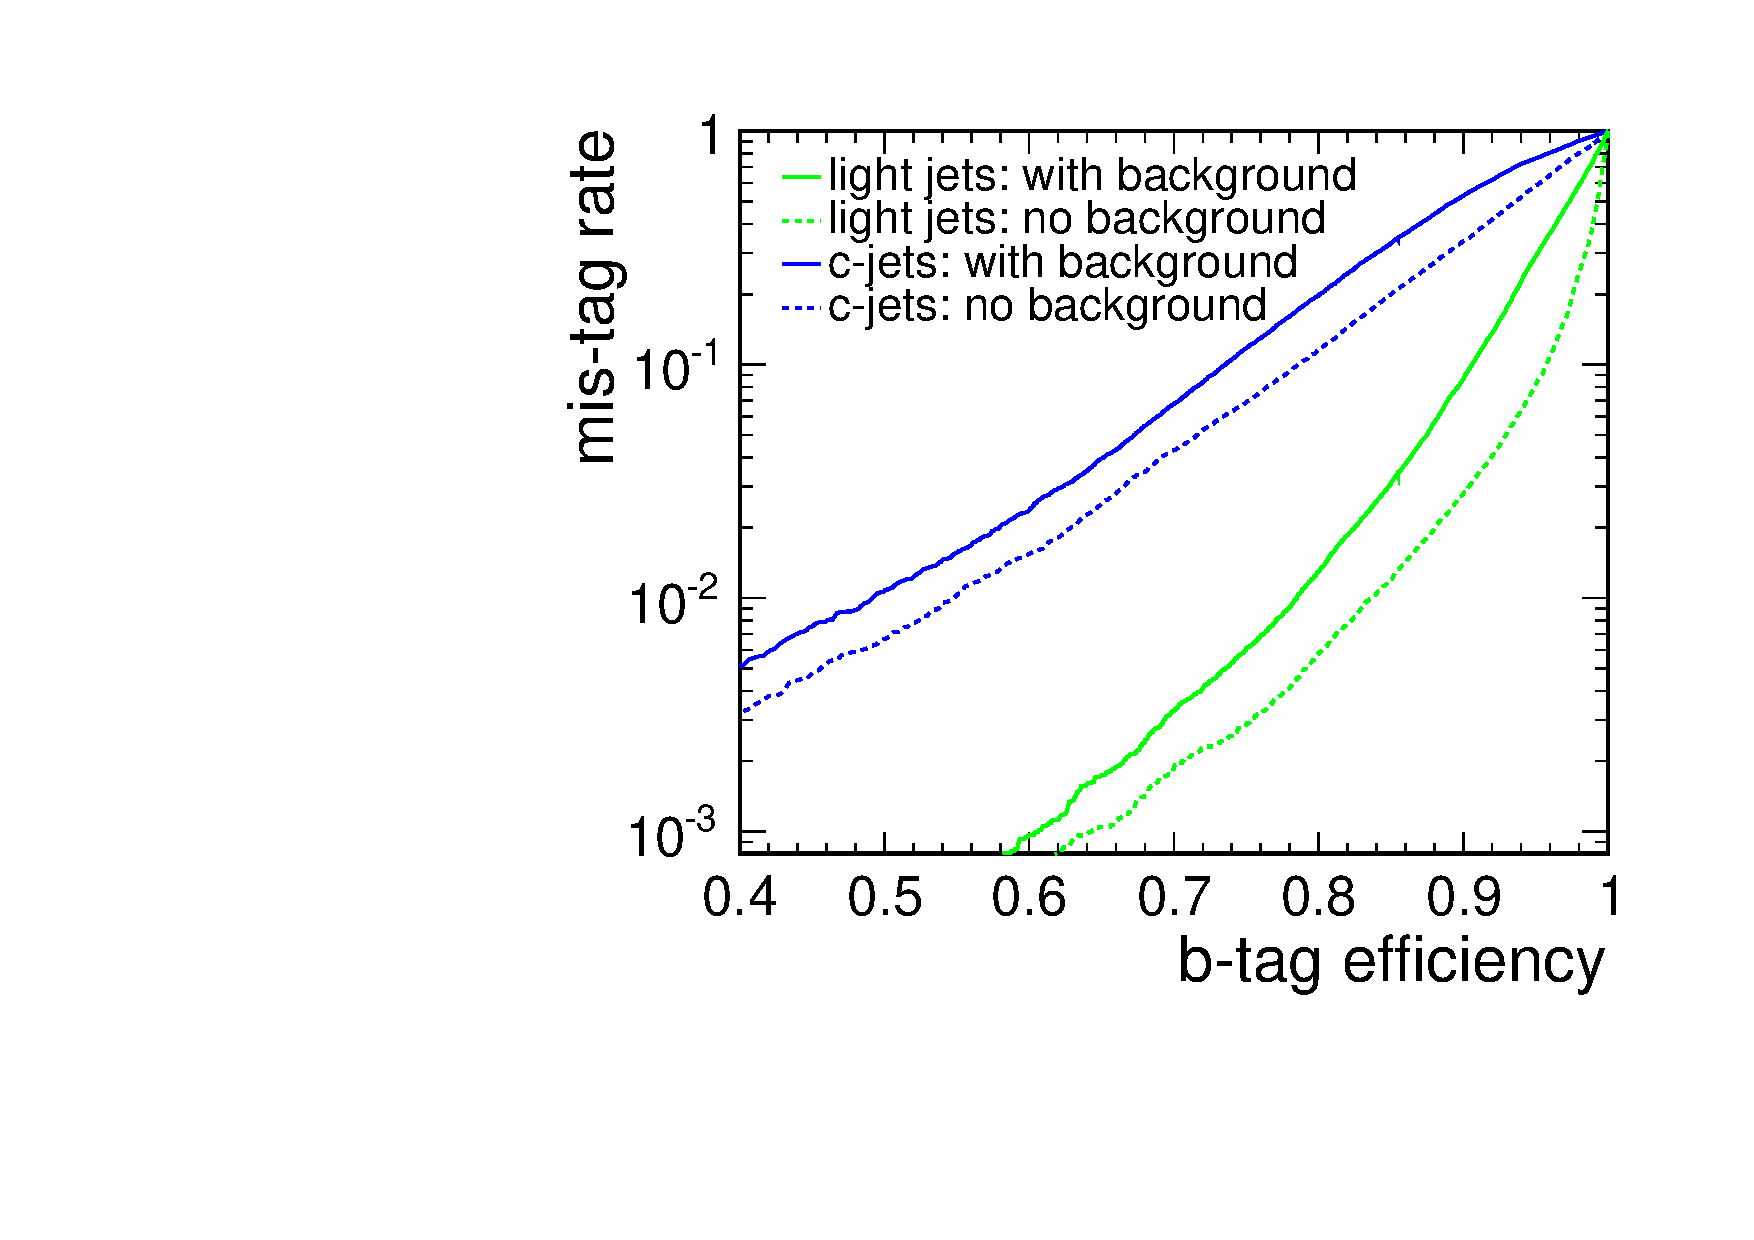
\includegraphics[width=4cm]{../SIDWorkshop/Light_Higgs_Flavour_Tag.pdf}
\column{4cm}
\centering
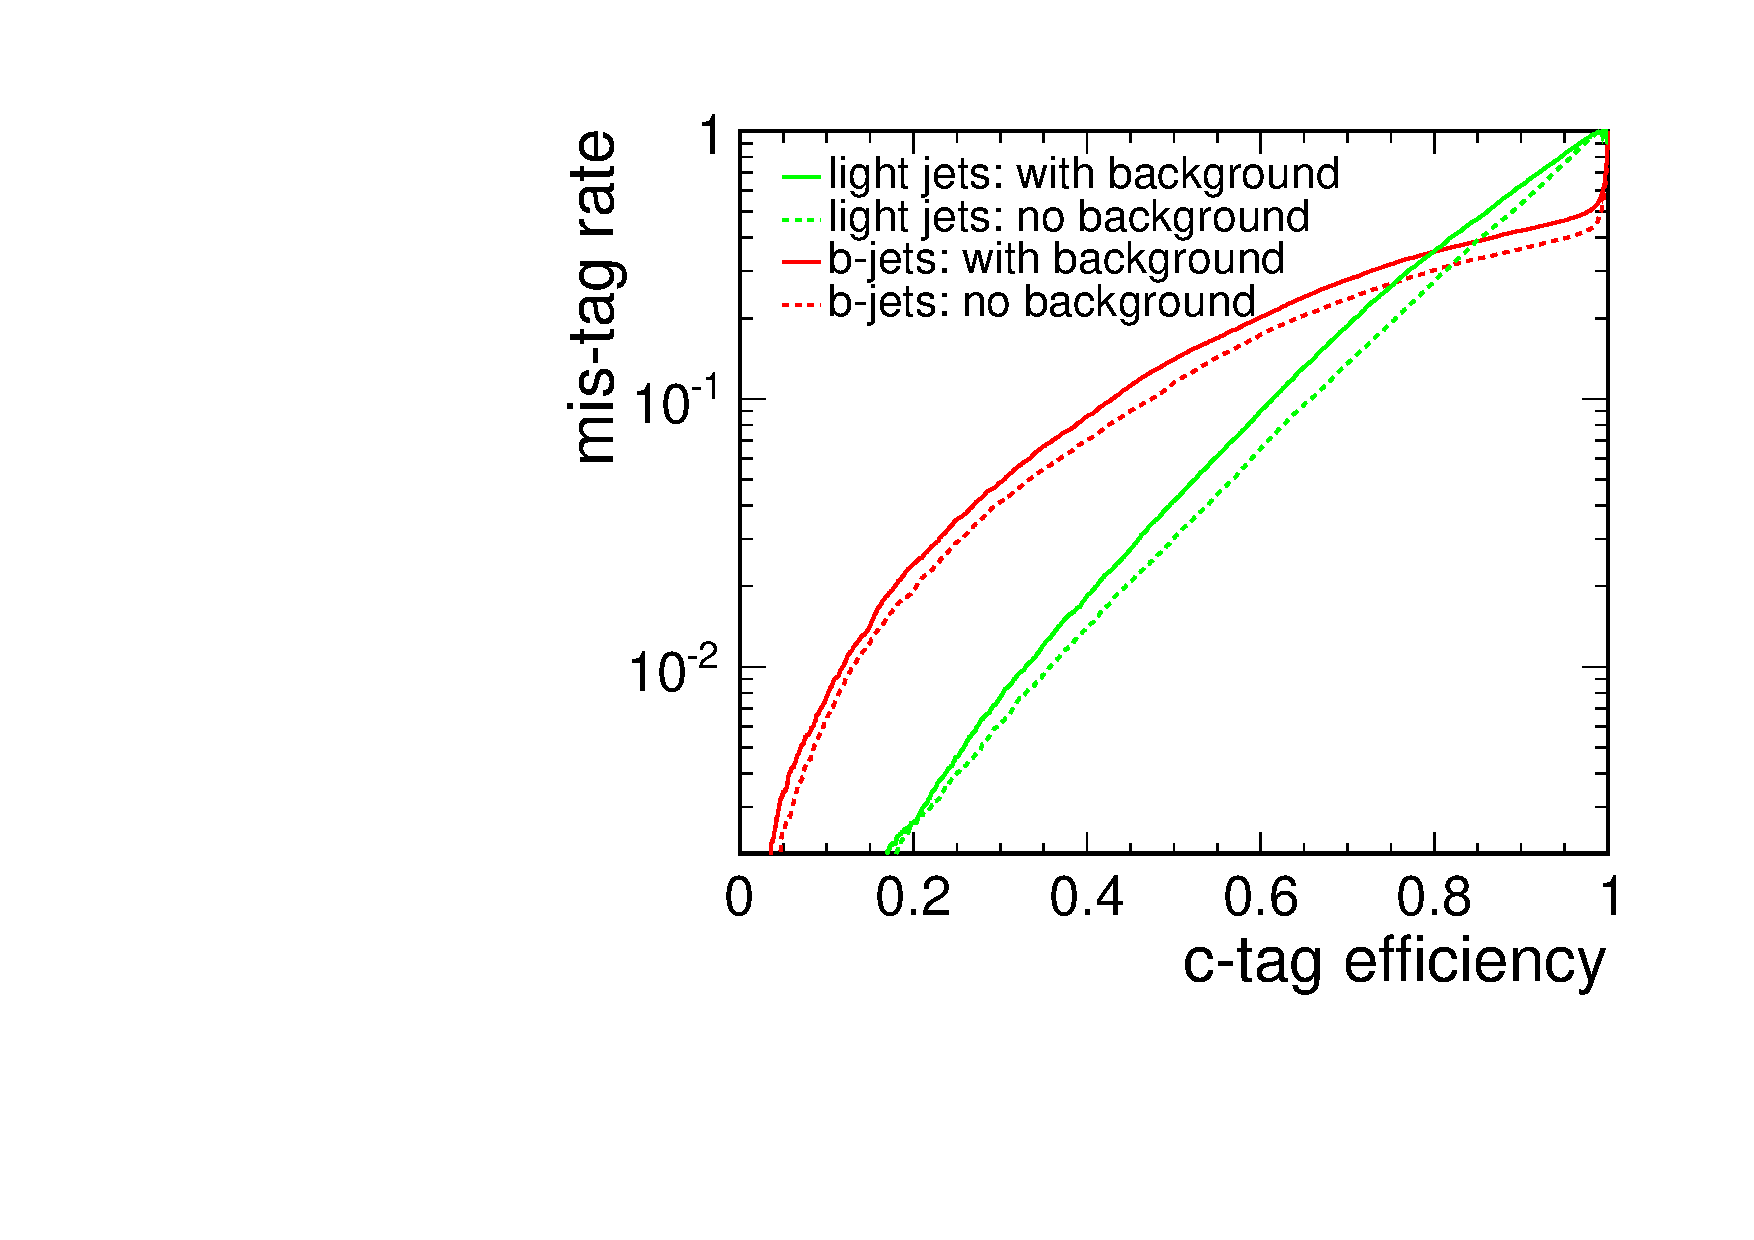
\includegraphics[width=4cm]{../SIDWorkshop/Light_Higgs_Flavour_Tag_C.pdf}
\end{columns}
Muon reconstruction efficiency ($\Ph\to\mu\mu$):
\begin{columns}[c]
\column{4cm}
\centering
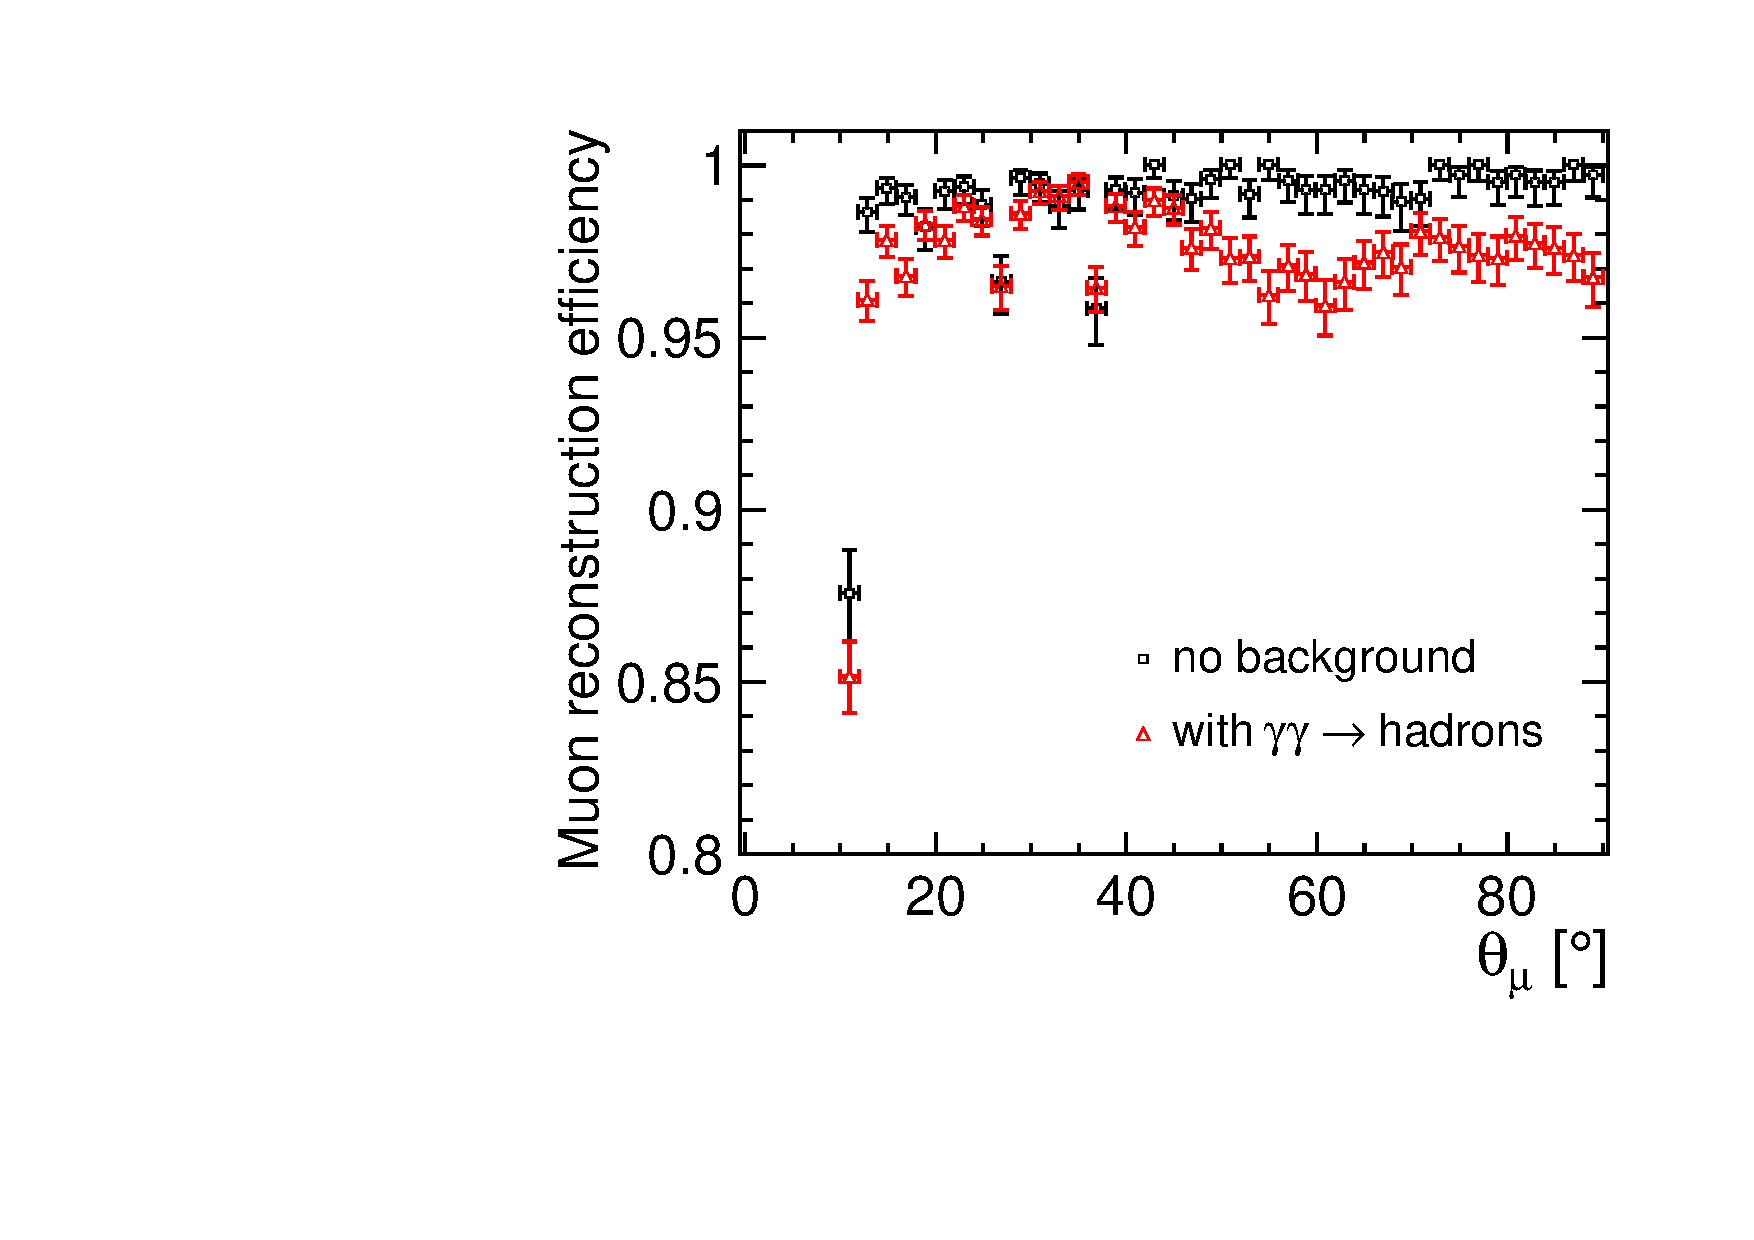
\includegraphics[width=4cm]{../SIDWorkshop/MuonEfficiency2.pdf}
\column{4cm}
\centering
%\includegraphics[width=4cm]{}
\end{columns}
\end{frame}

\begin{frame}
\frametitle{SM Higgs decays}
\begin{columns}[c]
\column{6cm}
\centering
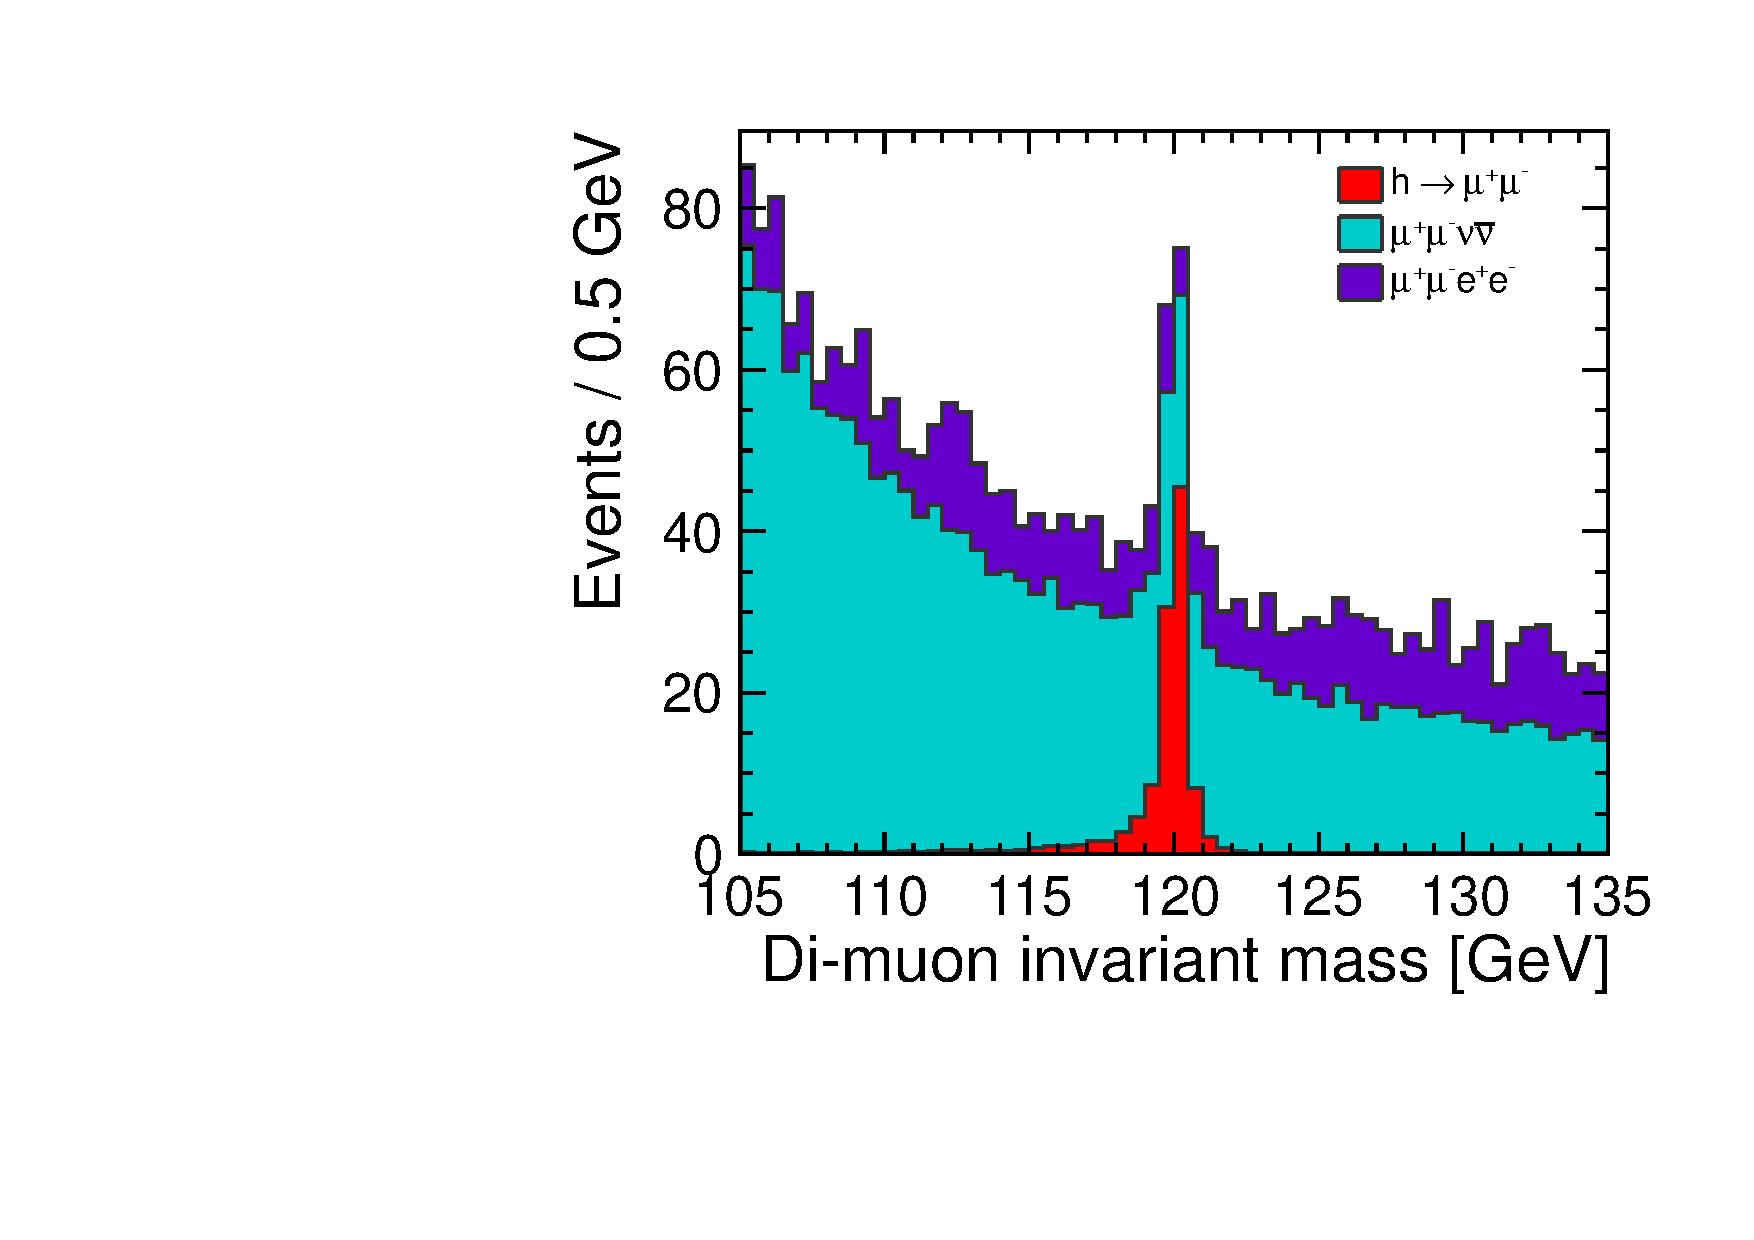
\includegraphics[width=5cm]{ee_h_mumu_mass_mh120GeV.pdf}
\column{6cm}
\centering
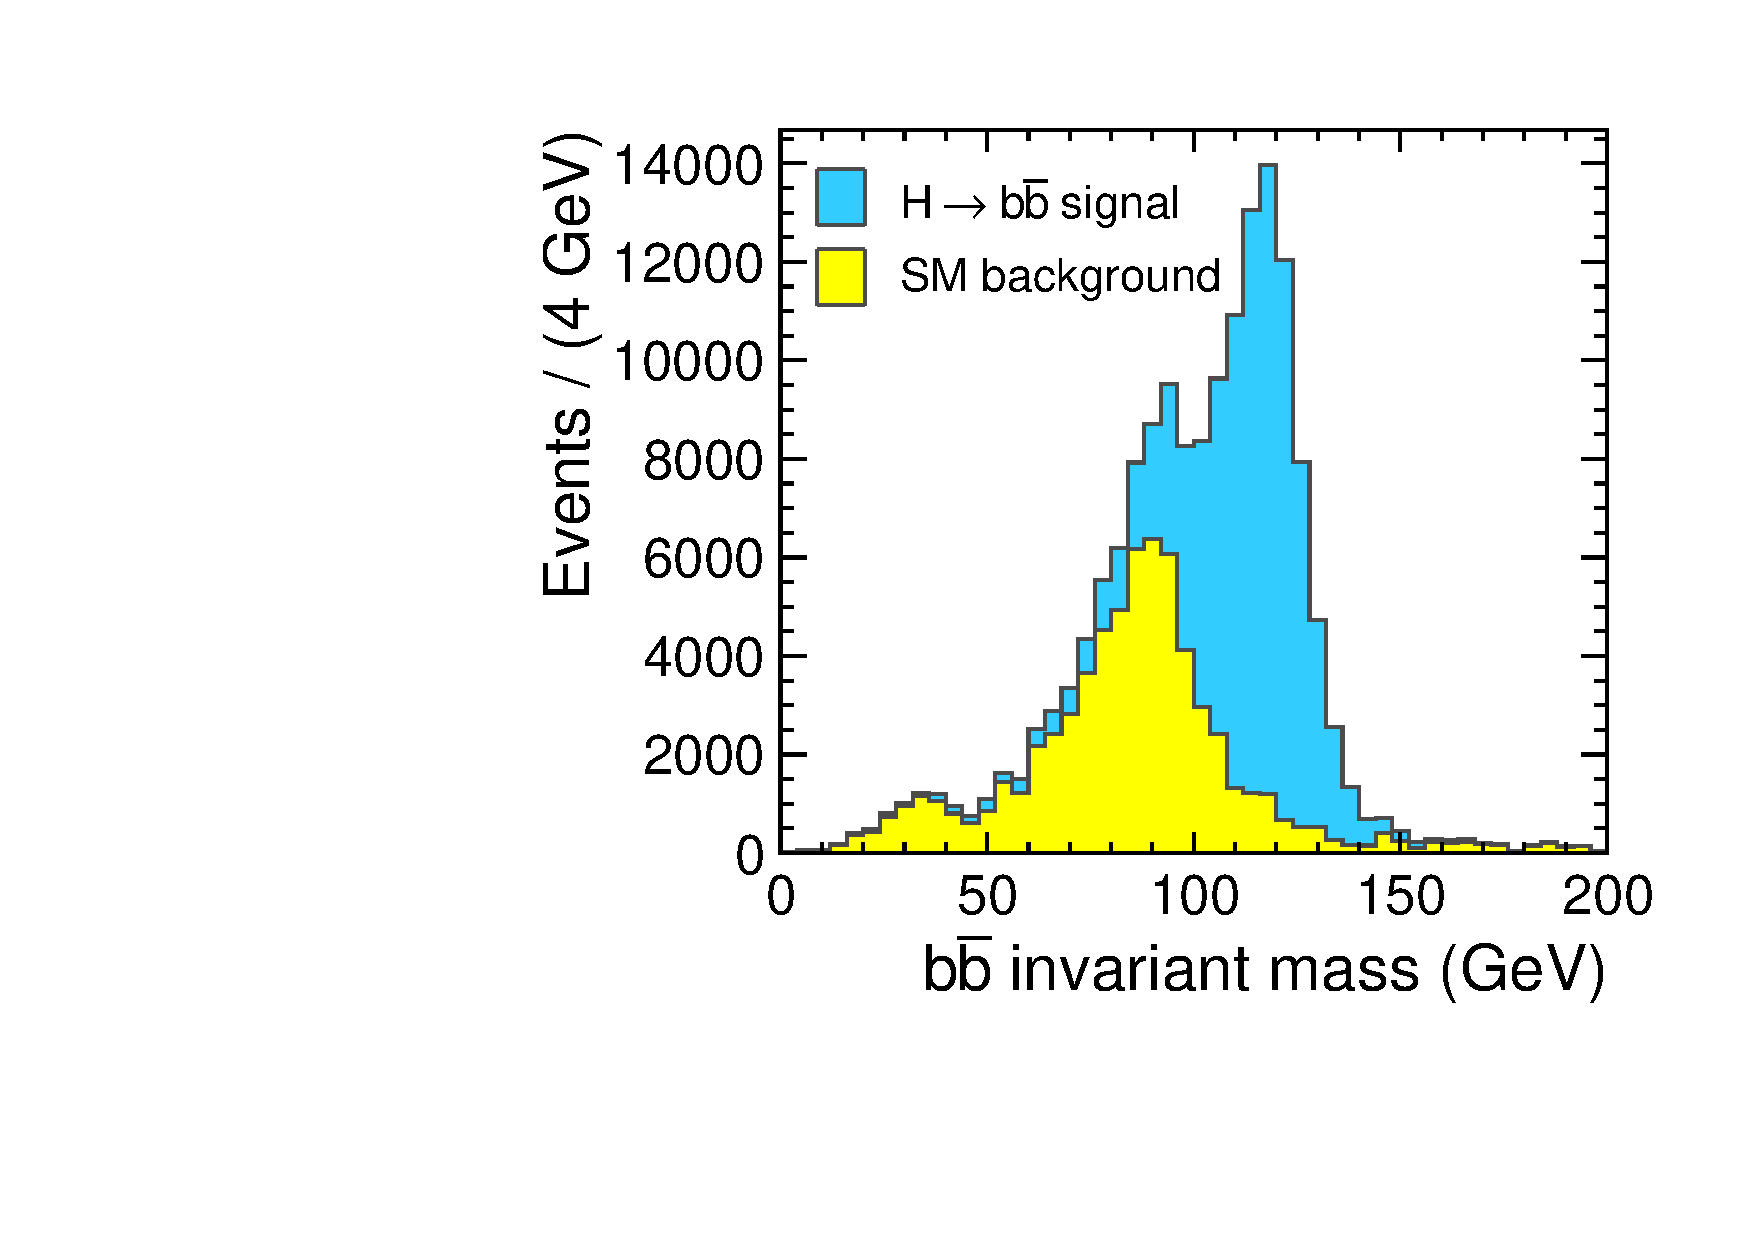
\includegraphics[width=5cm]{../SIDWorkshop/ee_h_bb_mass_mh120GeV}
\end{columns}
Cross section measurements:
\begin{itemize}
  \item
  $\sigma(\sigma_{\Ph\to\Pbottom\APbottom})/\sigma_{\Ph\to\Pbottom\APbottom} =
  0.22\%$ stat.
  \item $\sigma(\sigma_{\Ph\to\Pmuon\APmuon})/\sigma_{\Ph\to\Pmuon\APmuon}
  = 15.7\%$ stat.
\end{itemize}
\end{frame}

\begin{frame}
\frametitle{Heavy Higgs: $\PH^0\PA\to\Pbottom\APbottom\Pbottom\APbottom$,
$\PH^+\PH^-\to\Ptop\APbottom\Pbottom\APtop$}
\centering
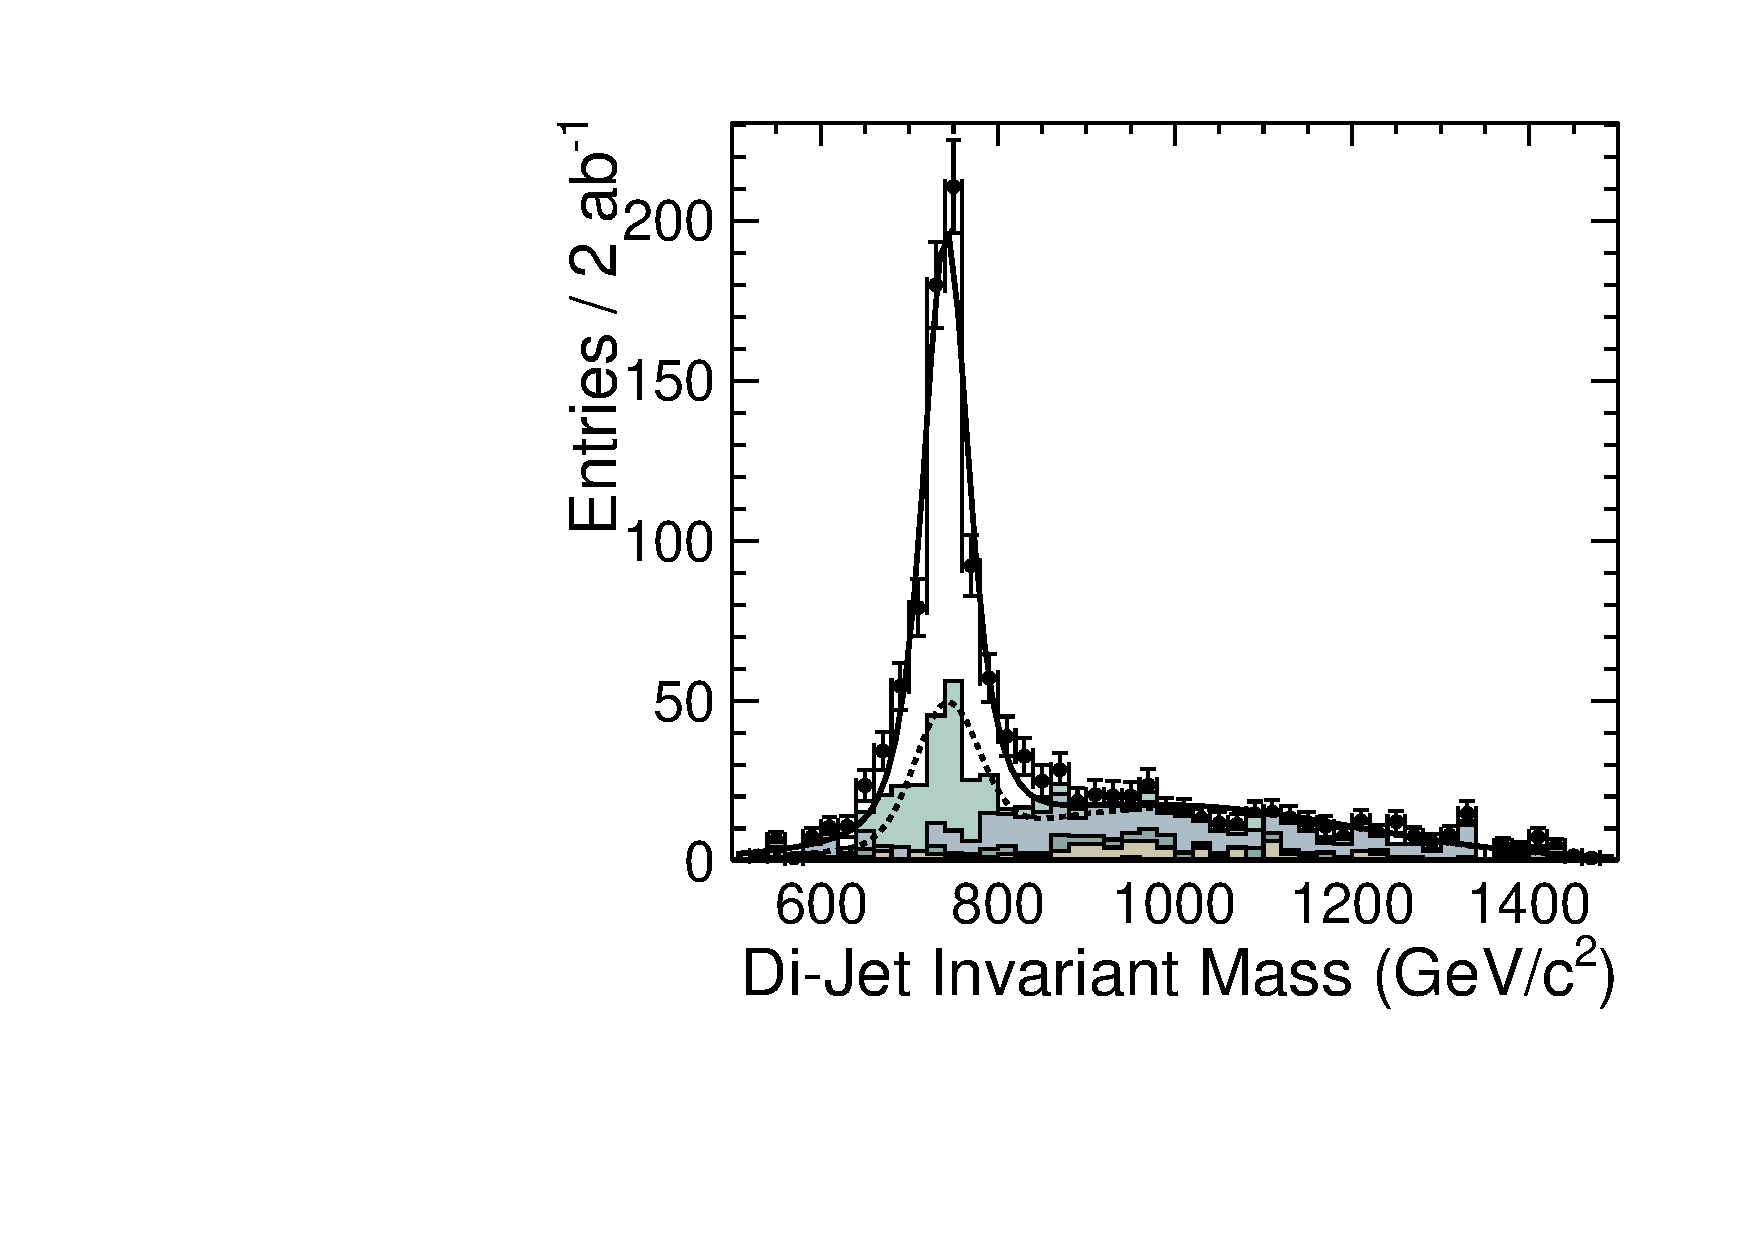
\includegraphics[width=4cm]{../SIDWorkshop/HAMass742_Bkg_CKFM_00BX_FJ.pdf}
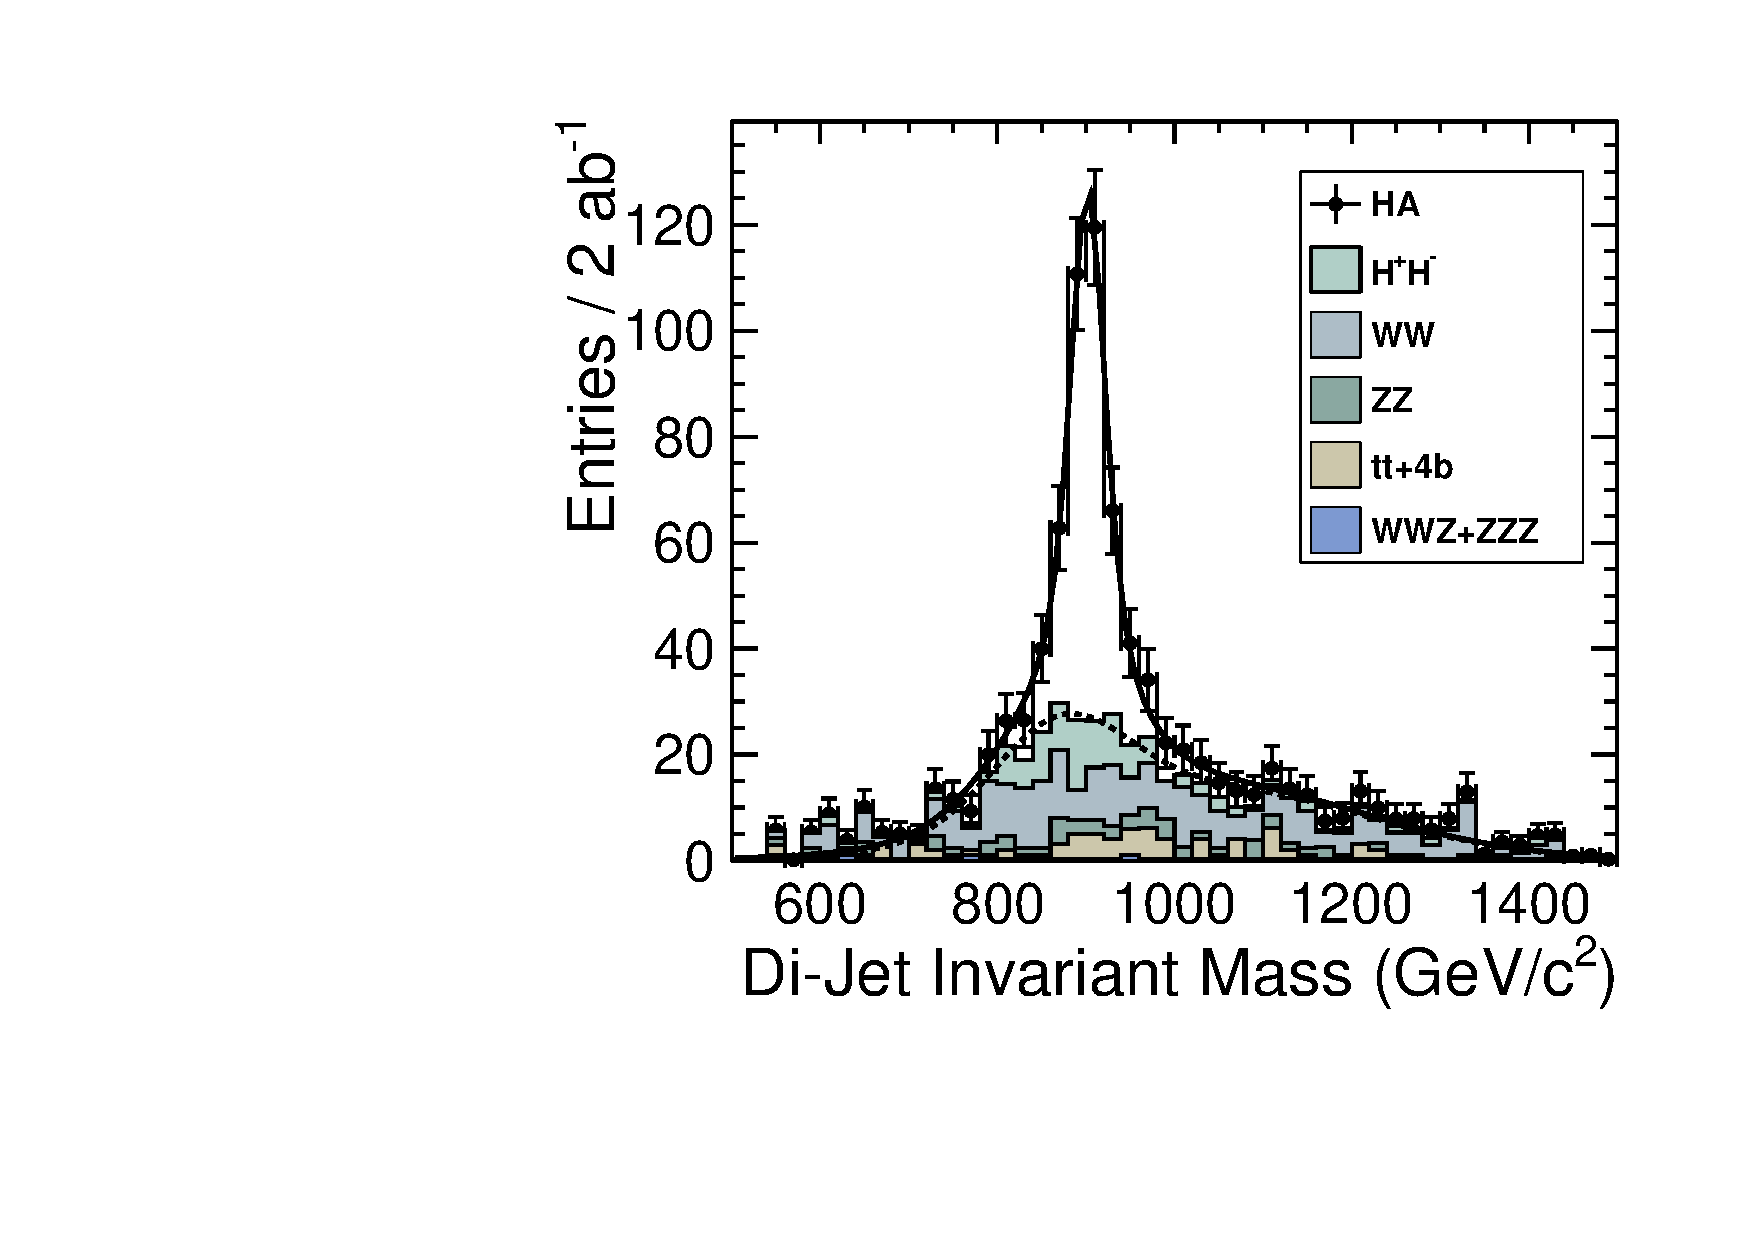
\includegraphics[width=4cm]{../SIDWorkshop/HAMass902_Bkg_CKFM_00BX_FJ.pdf}\\
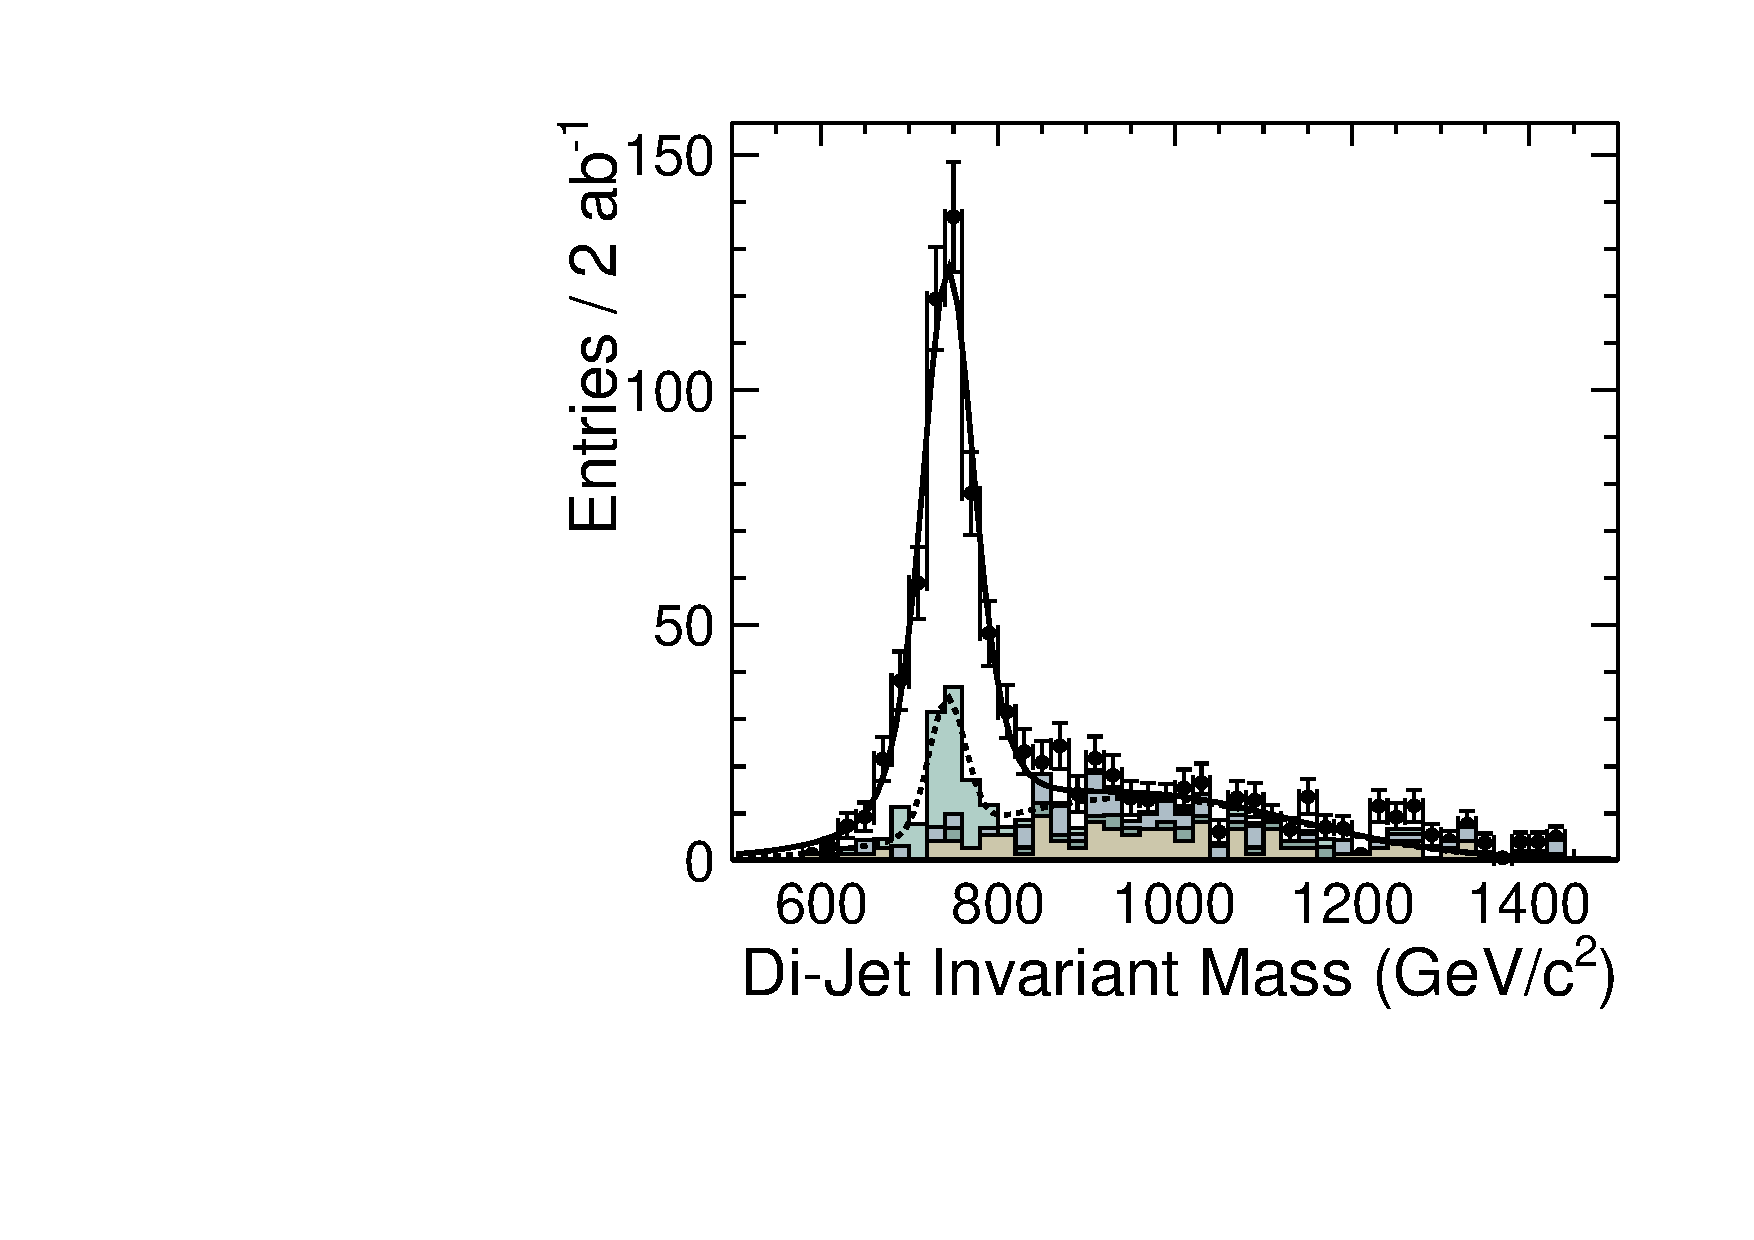
\includegraphics[width=4cm]{../SIDWorkshop/Hpm_Mass742_Bkg_CKFM_00BX_FJ.pdf}
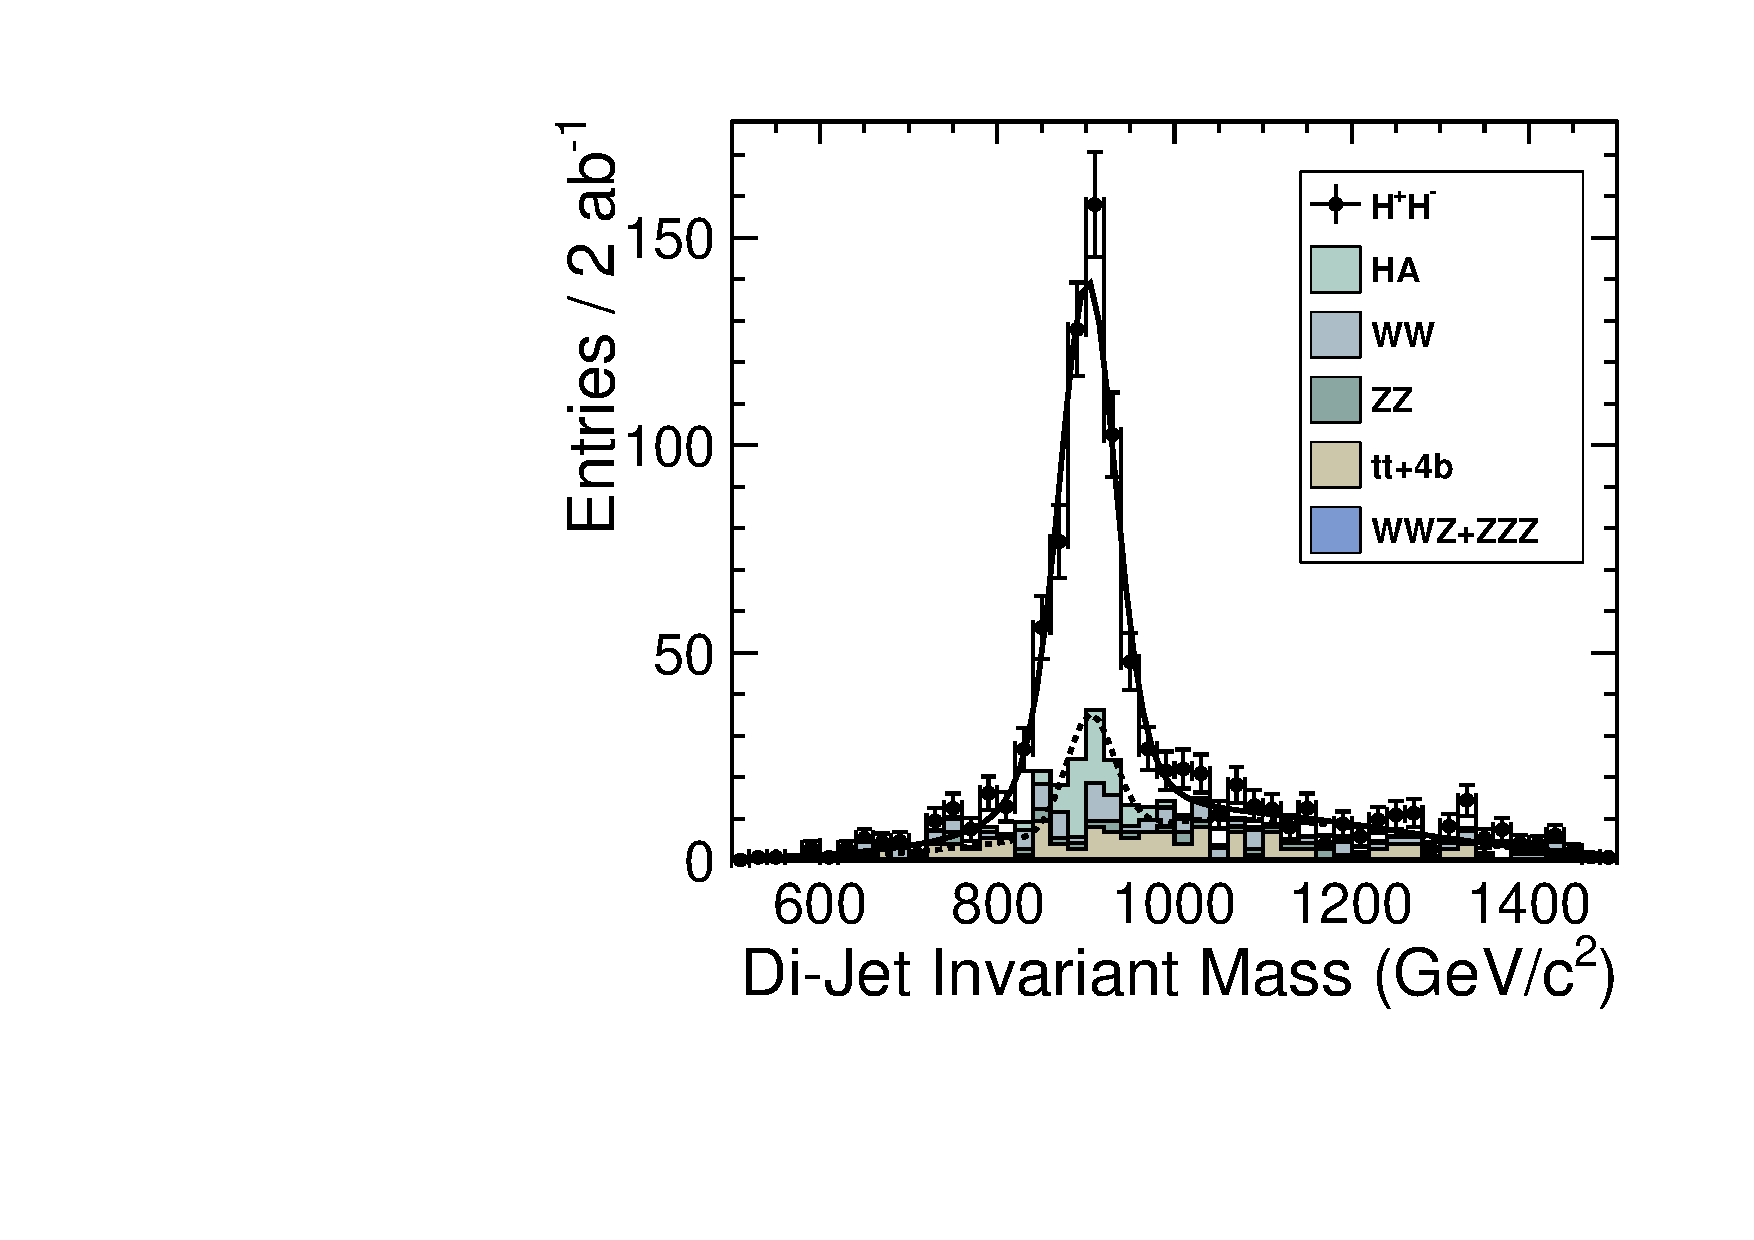
\includegraphics[width=4cm]{../SIDWorkshop/Hpm_Mass902_Bkg_CKFM_00BX_FJ.pdf}\\
{\scriptsize Statistical accuracy $\sigma(M)/M \sim0.3\%$.}\\
$\Rightarrow$ Evaluation of \alert{b-tagging and high energy jet
reconstruction}
\end{frame}

\begin{frame}
\frametitle{Squarks: $\Pep\Pem \to \PSq_R\PaSq_R\to\Pquark\APquark\PSgxz_1\PSgxz_1$} 
Used for \alert{jet and missing energy reconstruction} studies (see background
treatment)\\ Measuring $M_{\textrm{C}} = \sqrt{2(E_1E_2+\vec{p_1}.\vec{p_2})}$,
$M_{\textrm{C}}^{\textrm{max}}=\frac{m_{\PSq}^2 - m_{\chi}^2}{m_{\PSq}}$:
\begin{columns}[c]
\column{6cm}
\begin{center}
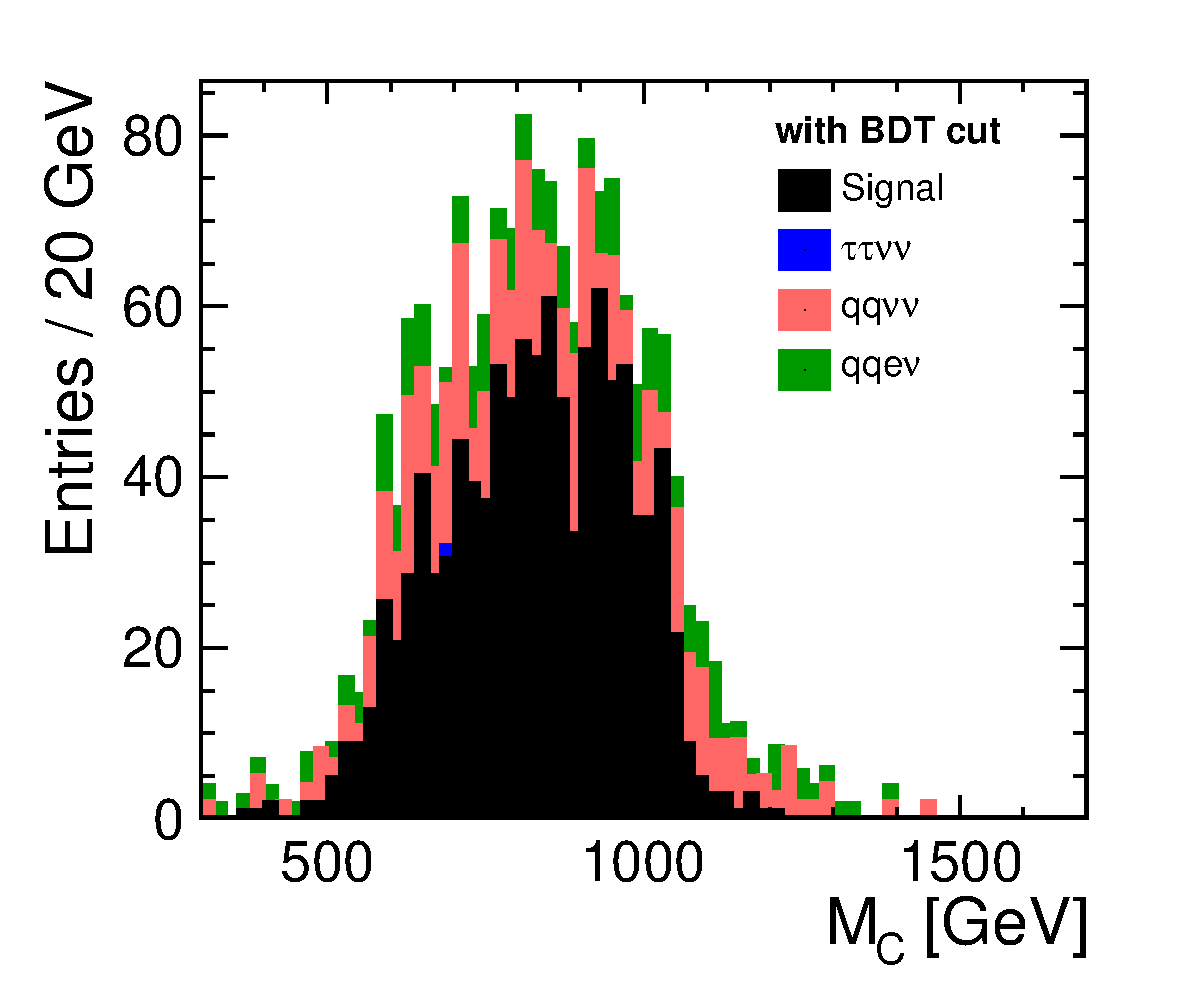
\includegraphics[width=6cm]{BackgroundRejection_MCwithBDTCut.pdf}\\
Selection cuts applied
\end{center}
\column{6cm}
From template fit using $2\textrm{ab}^{-1}$ ($\approx4$ years):\\
\begin{tabular}{cc}
\toprule
$\sigma(m_{\PSq})/m_{\PSq}$ & $0.5\%$\\
$\sigma(\textrm{xsec})/\textrm{xsec}$ & $5\%$\\
\bottomrule
\end{tabular}\\
~\\
\alert{Very high stat. precision!}
%\includegraphics{}
\end{columns}
\end{frame}
\begin{frame}
\frametitle{Sleptons: $\Pep\Pem \to \PSl \PaSl \,(\ell = \Pe,\Pgm,\Pgne)$}
Probe of \alert{lepton ID and reconstruction}
\begin{columns}[c]
\column{3.8cm}
\begin{center}
Selectrons\\
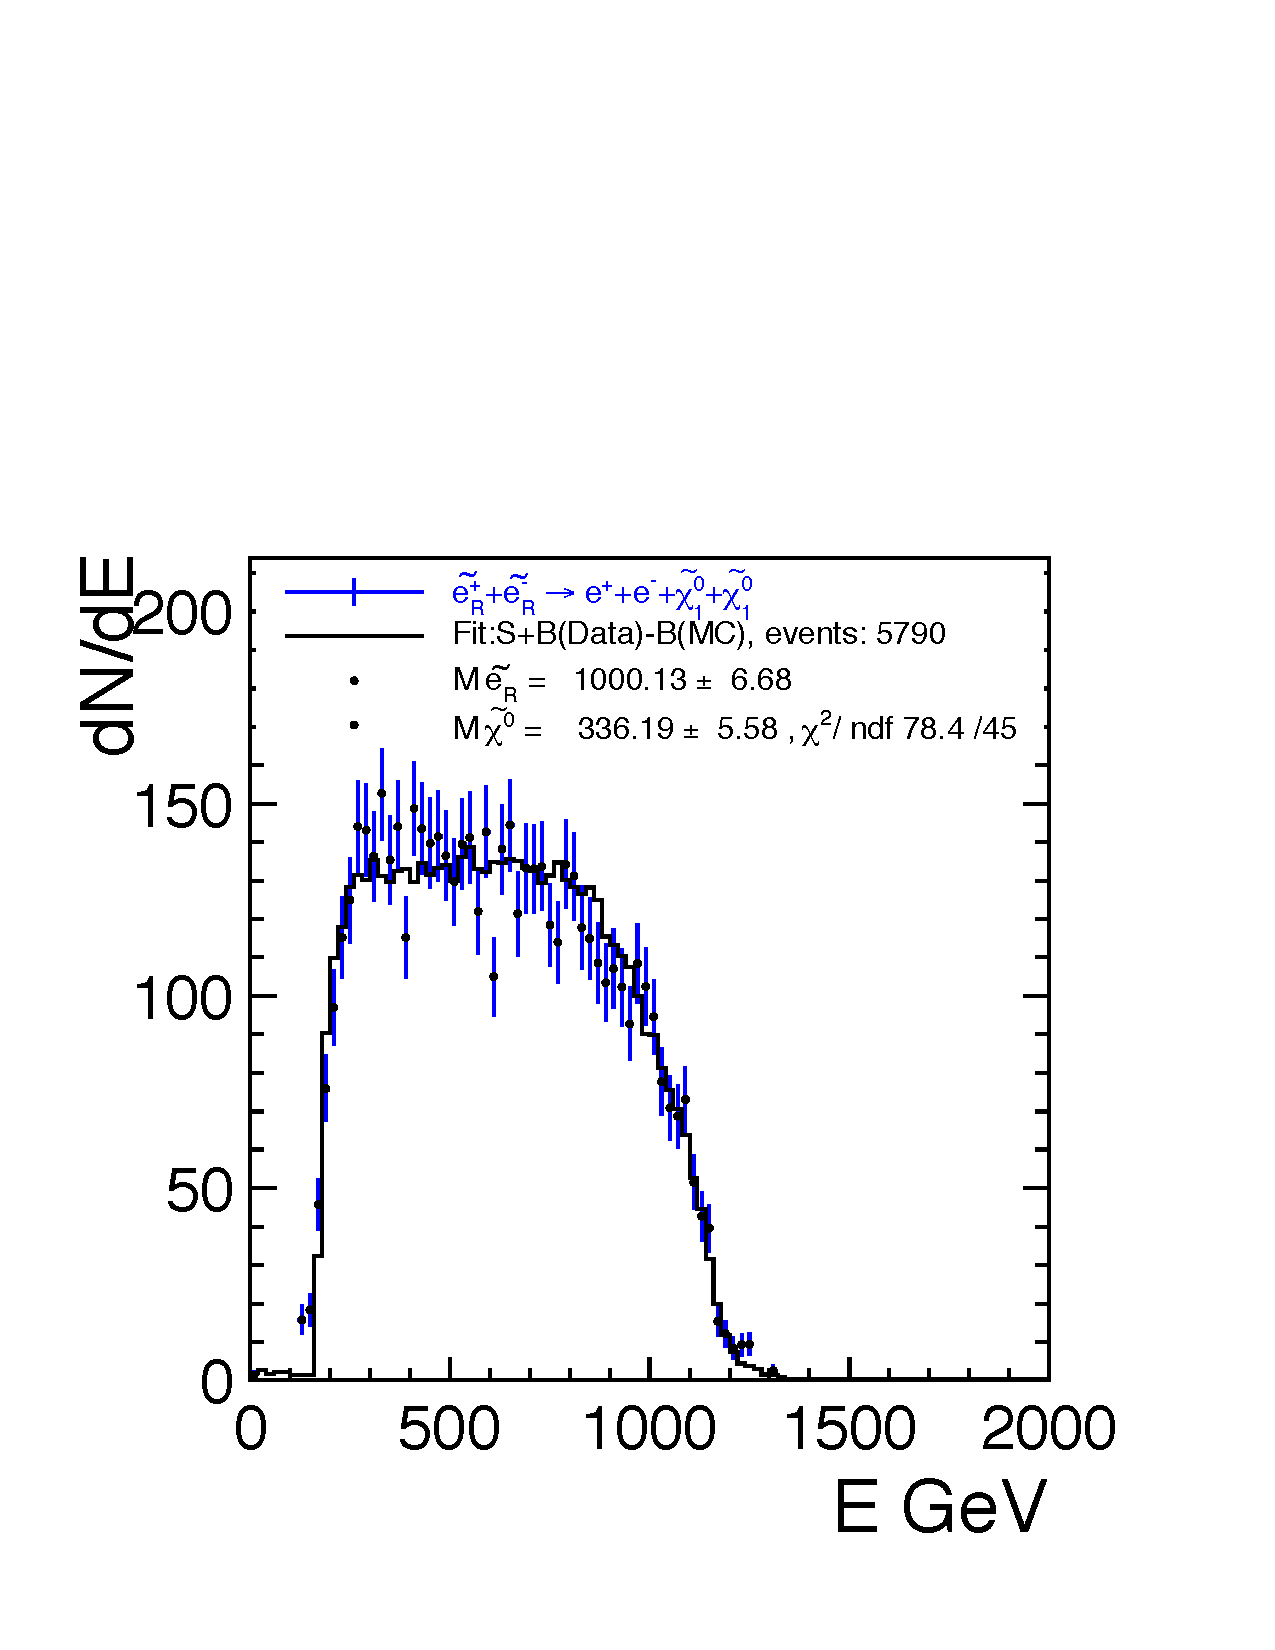
\includegraphics[width=3.8cm]{202_H1LPADC4.pdf}
\end{center}
\column{4.6cm}
\begin{center}
Smuons\\
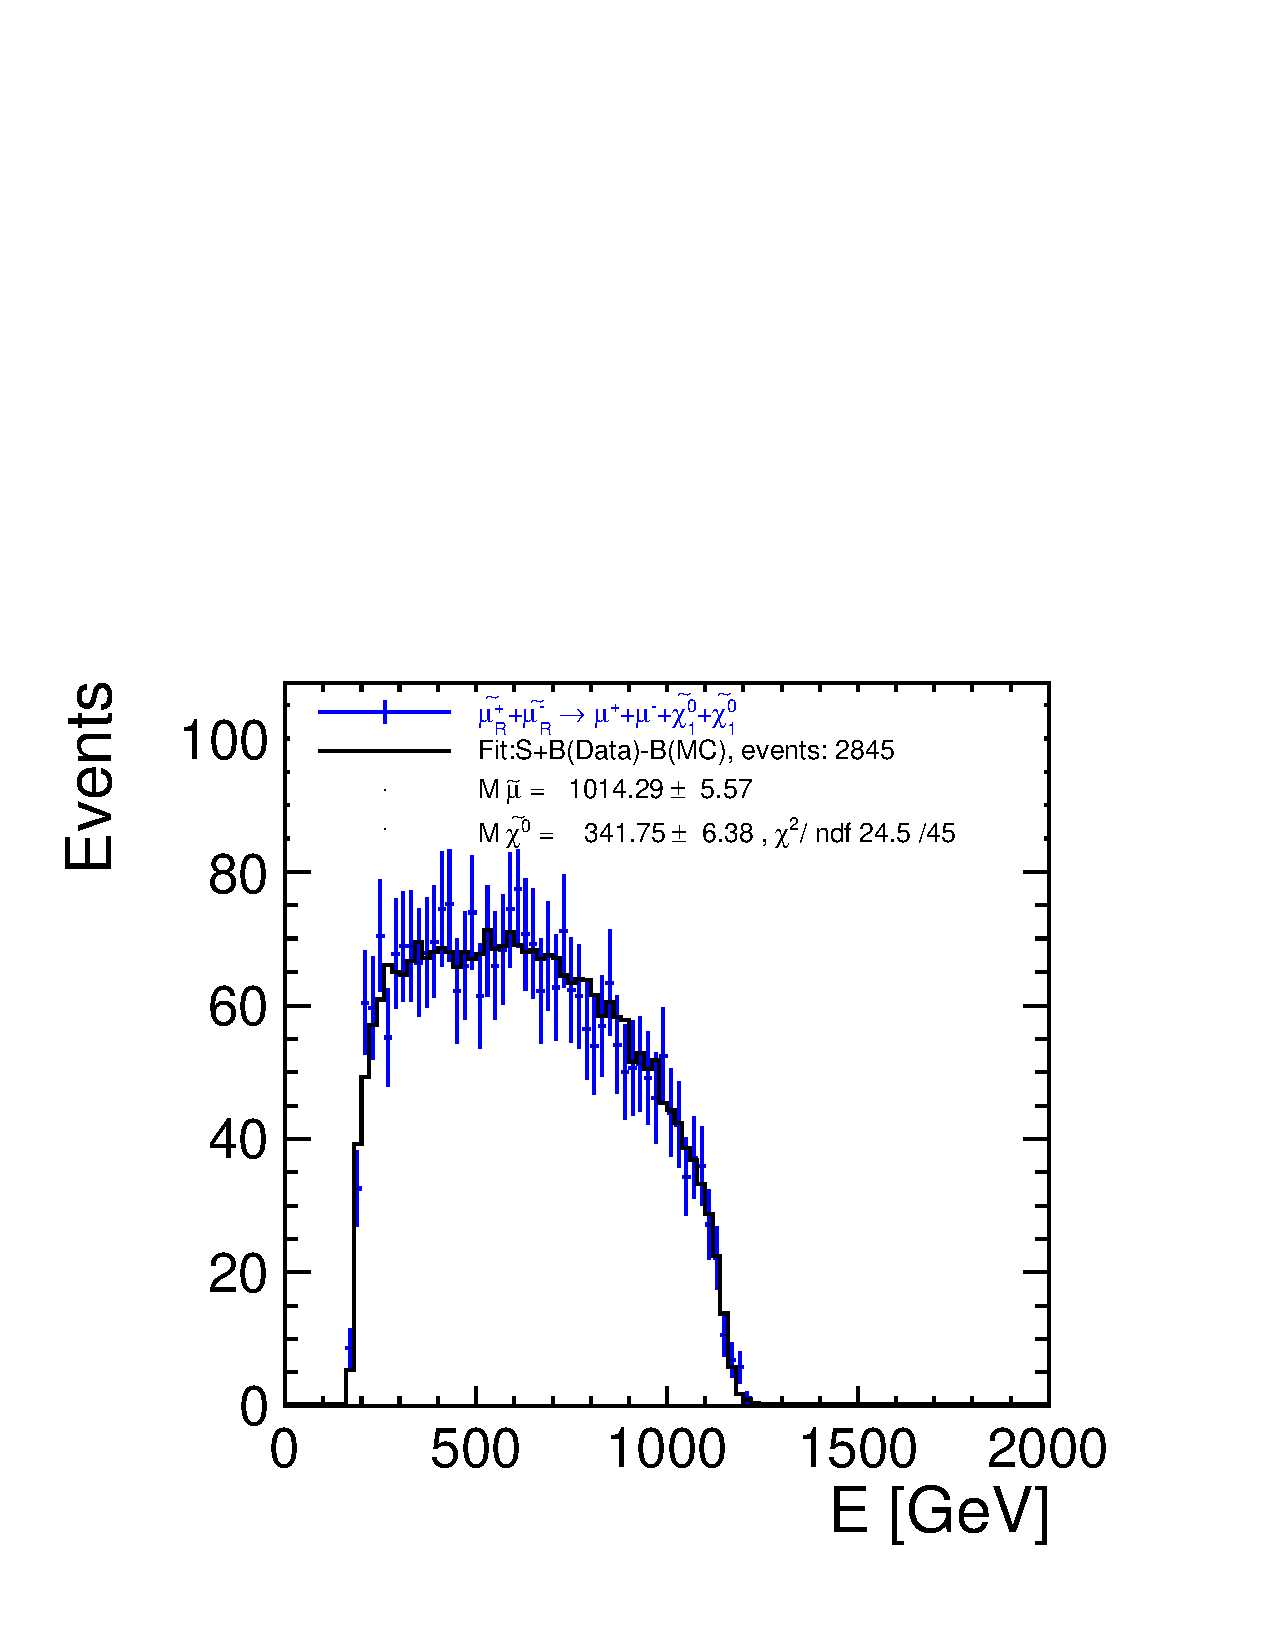
\includegraphics[width=4.6cm]{205_H1LPADC4.pdf}
\end{center}
\column{4.6cm}
\begin{center}
Sneutrinos\\
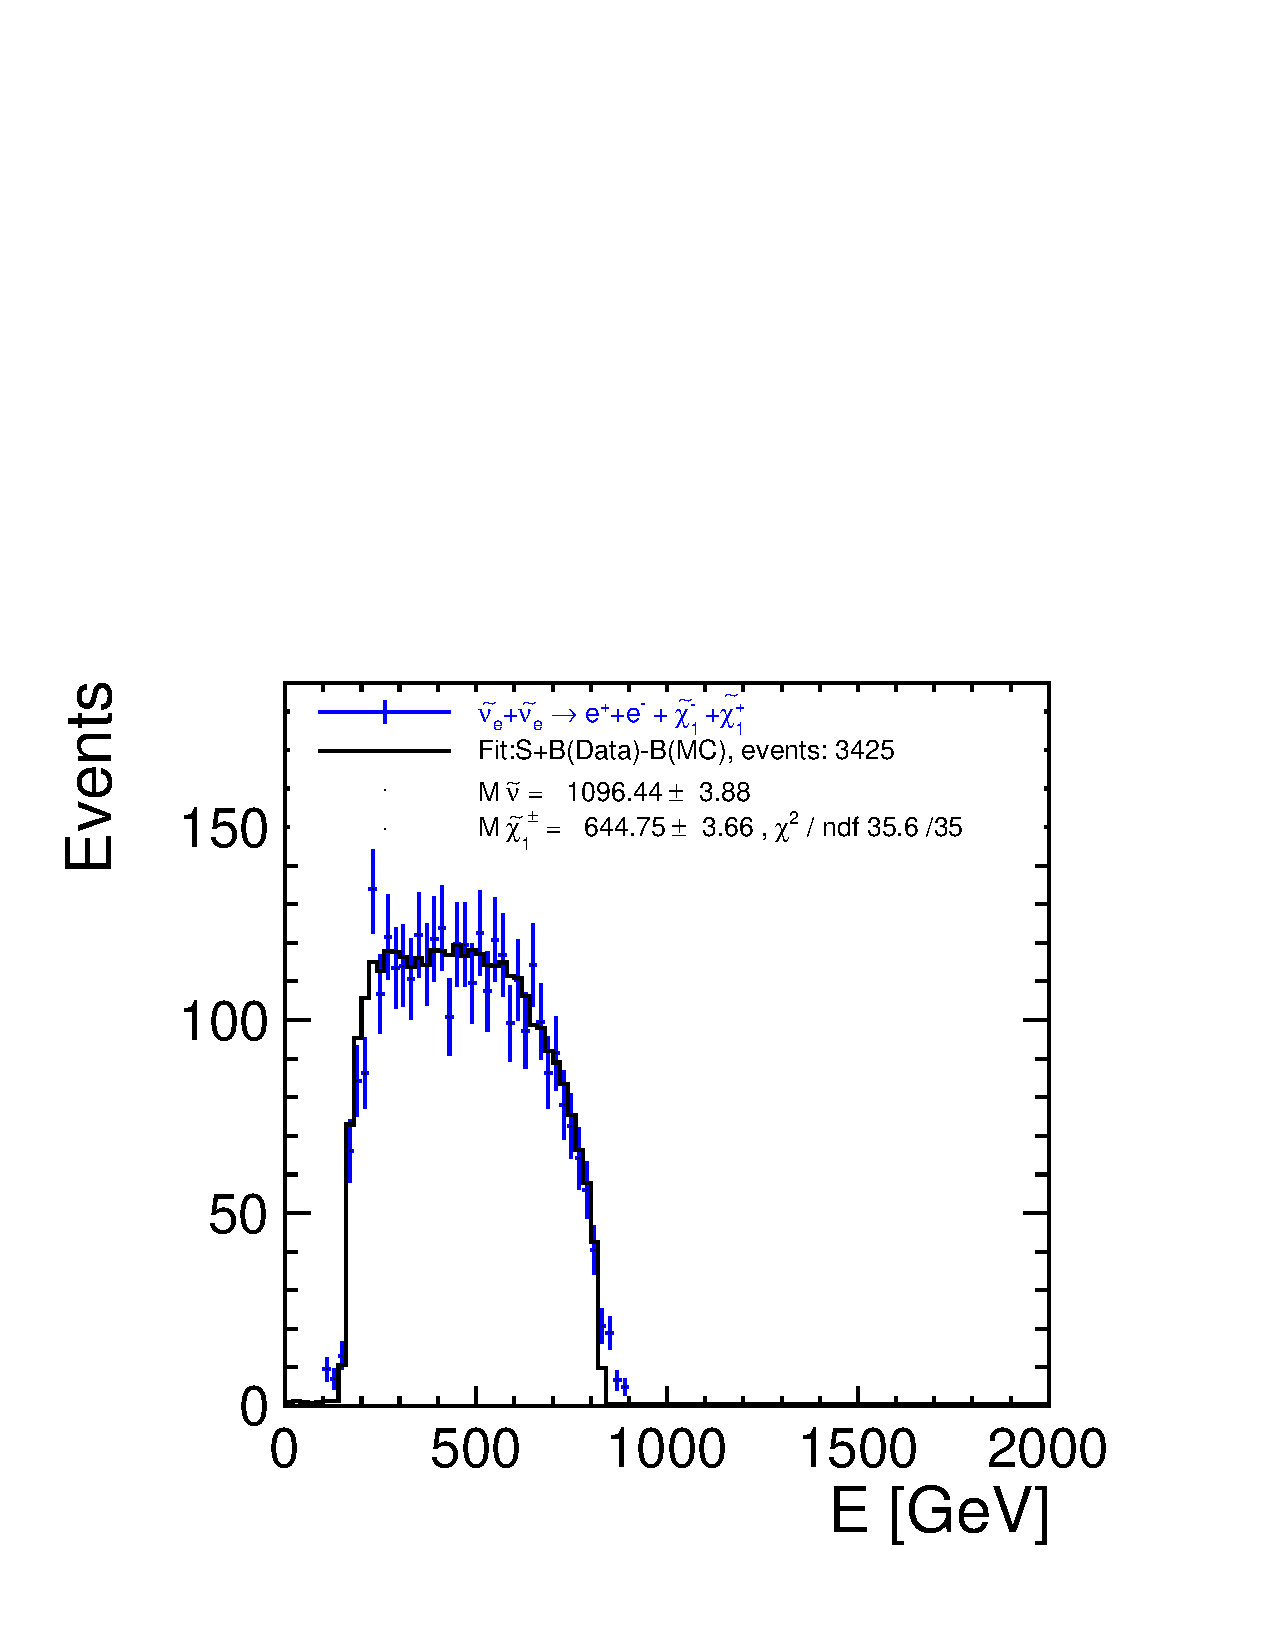
\includegraphics[width=4.6cm]{213_H1LPADC4.pdf}
\end{center}
\end{columns}
~\\
Mass obtained from the end points
\end{frame}
\begin{frame}
\frametitle{Sleptons: $\Pep\Pem \to \PSl \PaSl \,(\ell = \Pe,\Pgm,\Pgne)$}
With $2\textrm{ab}^{-1}$:
\begin{center}
\begin{tabular}{ccc}
process & $\sigma(\textrm{xsec})/\textrm{xsec}$ & $\sigma(m_{\PSl})/m_{\PSl}$\\
\midrule
$\Pep\Pem \to \PSgm_R\bar{\PSgm_R} \to \mu^+\mu^-\PSgxz_1\PSgxz_1$ & 2.8\%
&0.6\%\\ $\Pep\Pem \to \PSe_R\bar{\PSe_R} \to \Pep\Pem\PSgxz_1\PSgxz_1$ & 0.8\% & 0.3\%\\
$\Pep\Pem \to \PSgn_{\textrm{e}}\bar{\PSgn_{\textrm{e}}} \to
\Pep\Pem\PSgx^+_1\PSgx^-_1$ & $\sim2.4\%$ & $\sim0.4\%$ \\ $\Pep\Pem \to \PSe_L\bar{\PSe_L} \to \Pep\Pem\PSgxz_2\PSgxz_2$ & $\sim7.0\%$ &
-\\
\bottomrule
\end{tabular}
\end{center}
\alert{Very high stat. precision!}
\end{frame}

\begin{frame}
\frametitle{Gauginos}
{\footnotesize $\Pep\Pem \to \PSgxpm_1 \PSgxmp_1\to\PWp\PWm\PSgxz_1\PSgxz_1$ and
$\Pep\Pem \to \PSgxz_2 \PSgxz_2\to \Ph\Ph\PSgxz_1\PSgxz_1$}
\begin{columns}[c]
\column{6cm}
\centering
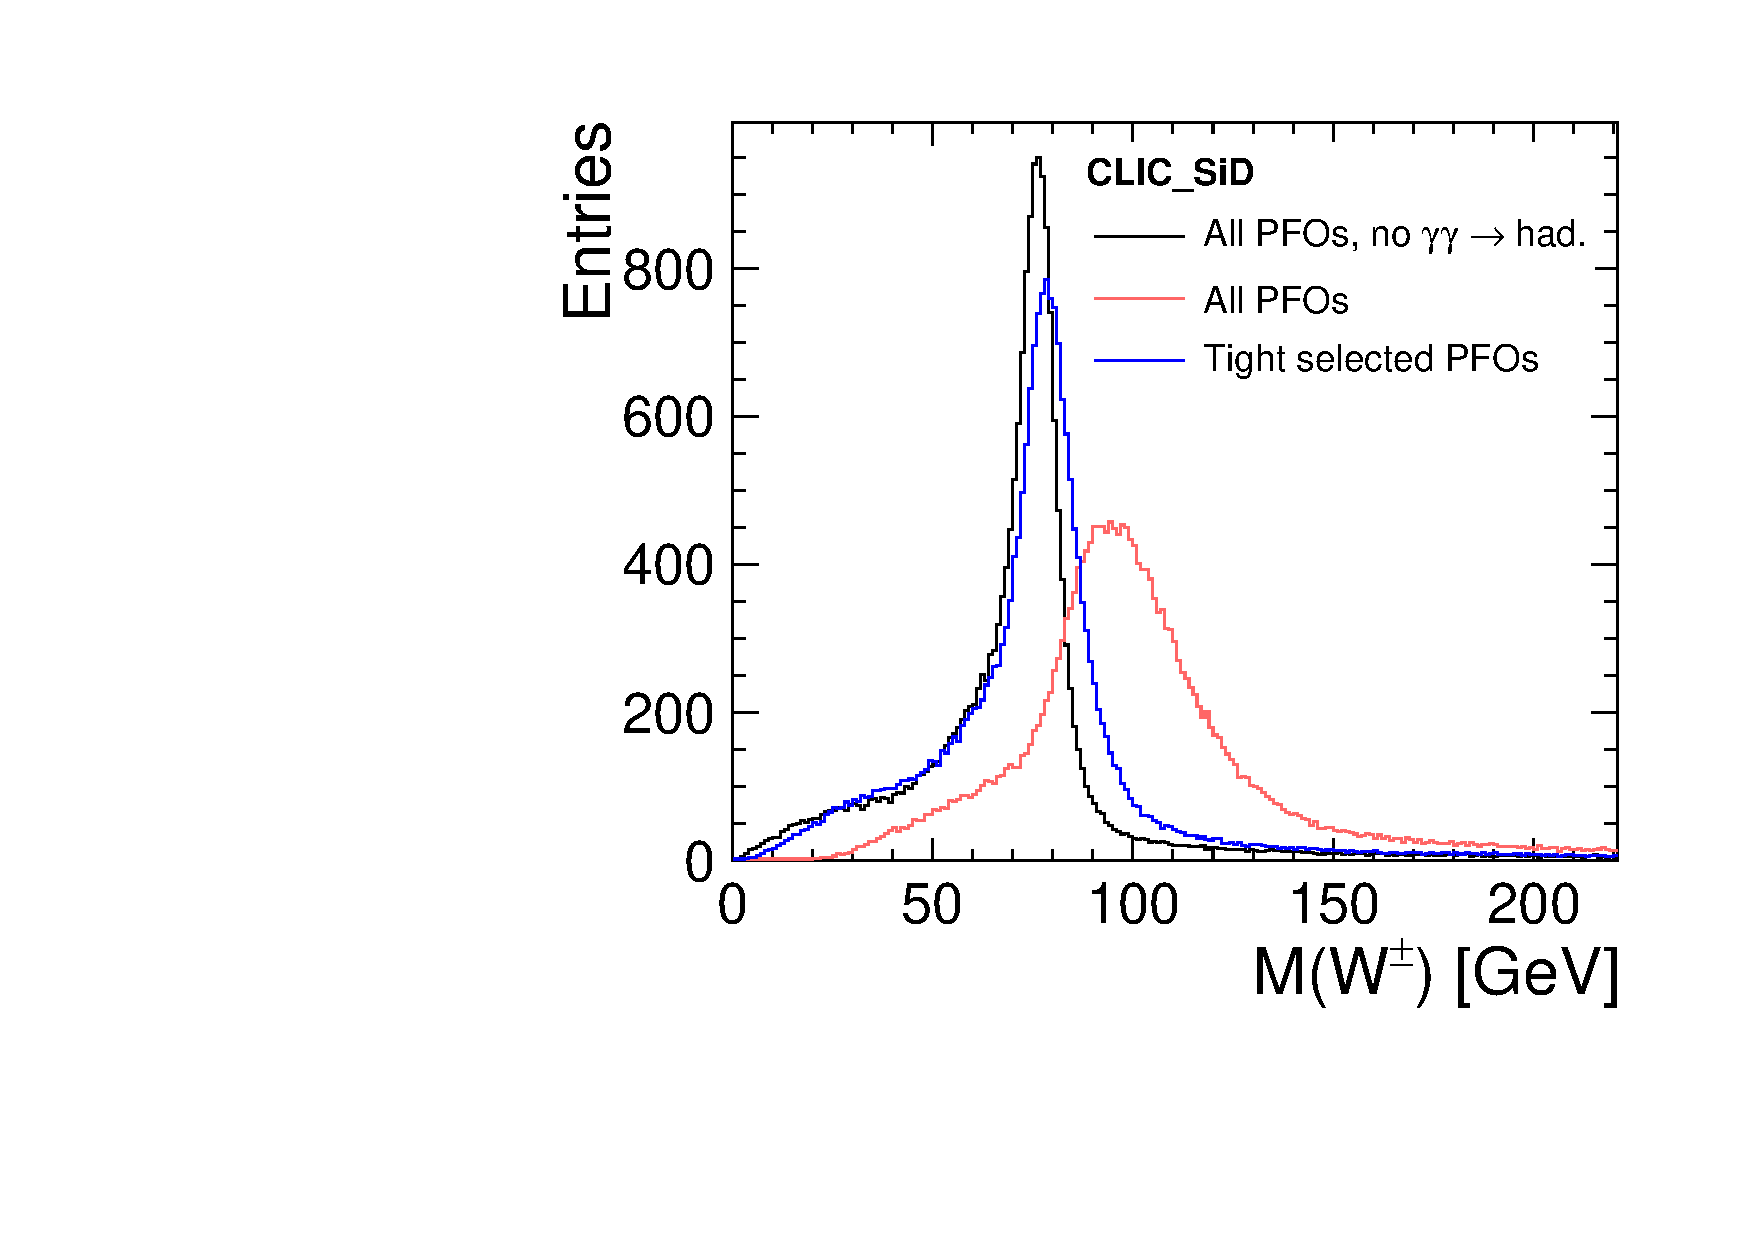
\includegraphics[width=6cm]{../SIDWorkshop/W_reconstruction_mass.pdf}
\column{6cm}
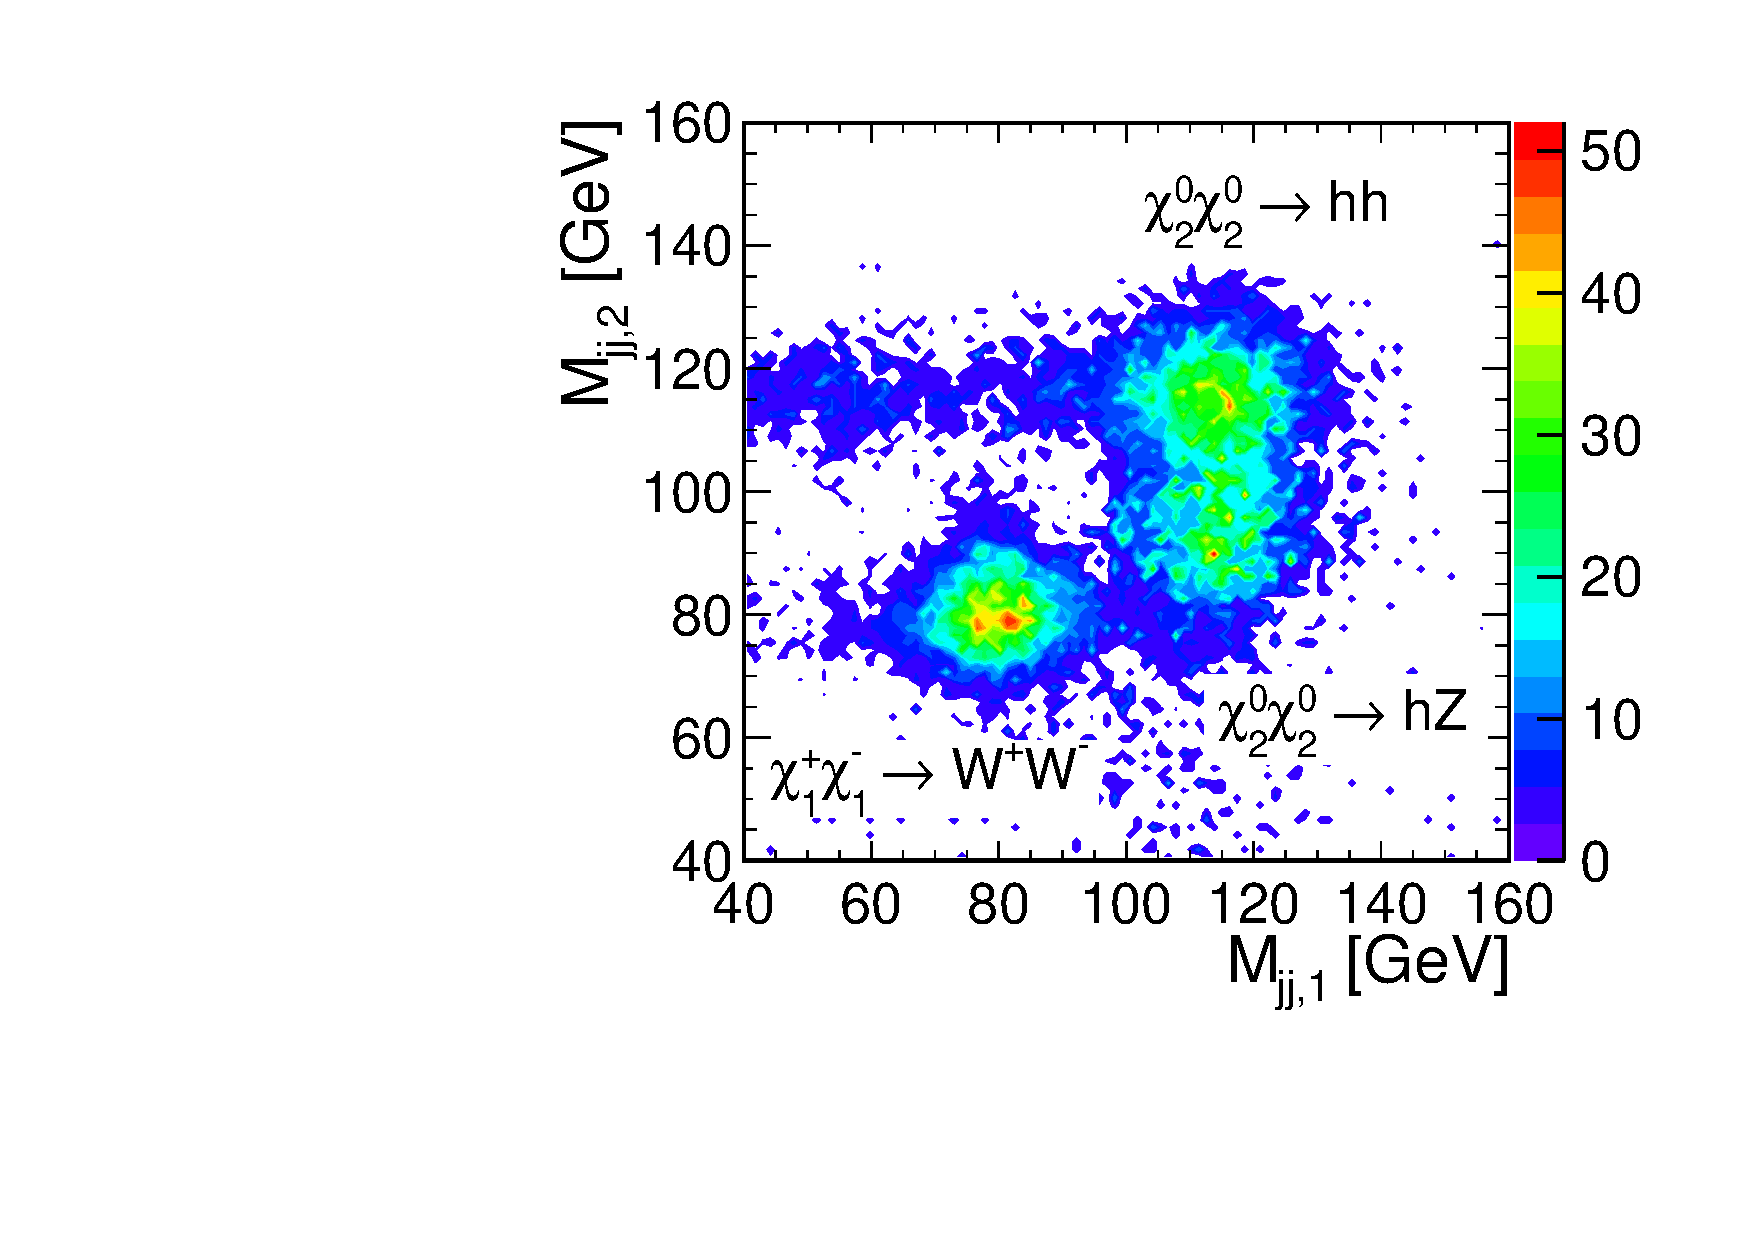
\includegraphics[width=6cm]{../WhizardWorkshop/MassPlot2D}
\end{columns}
\alert{Test of jet energy resolution}
\end{frame}
\begin{frame}
\frametitle{Gauginos}
\begin{columns}[c]
\column{4.5cm}
\centering
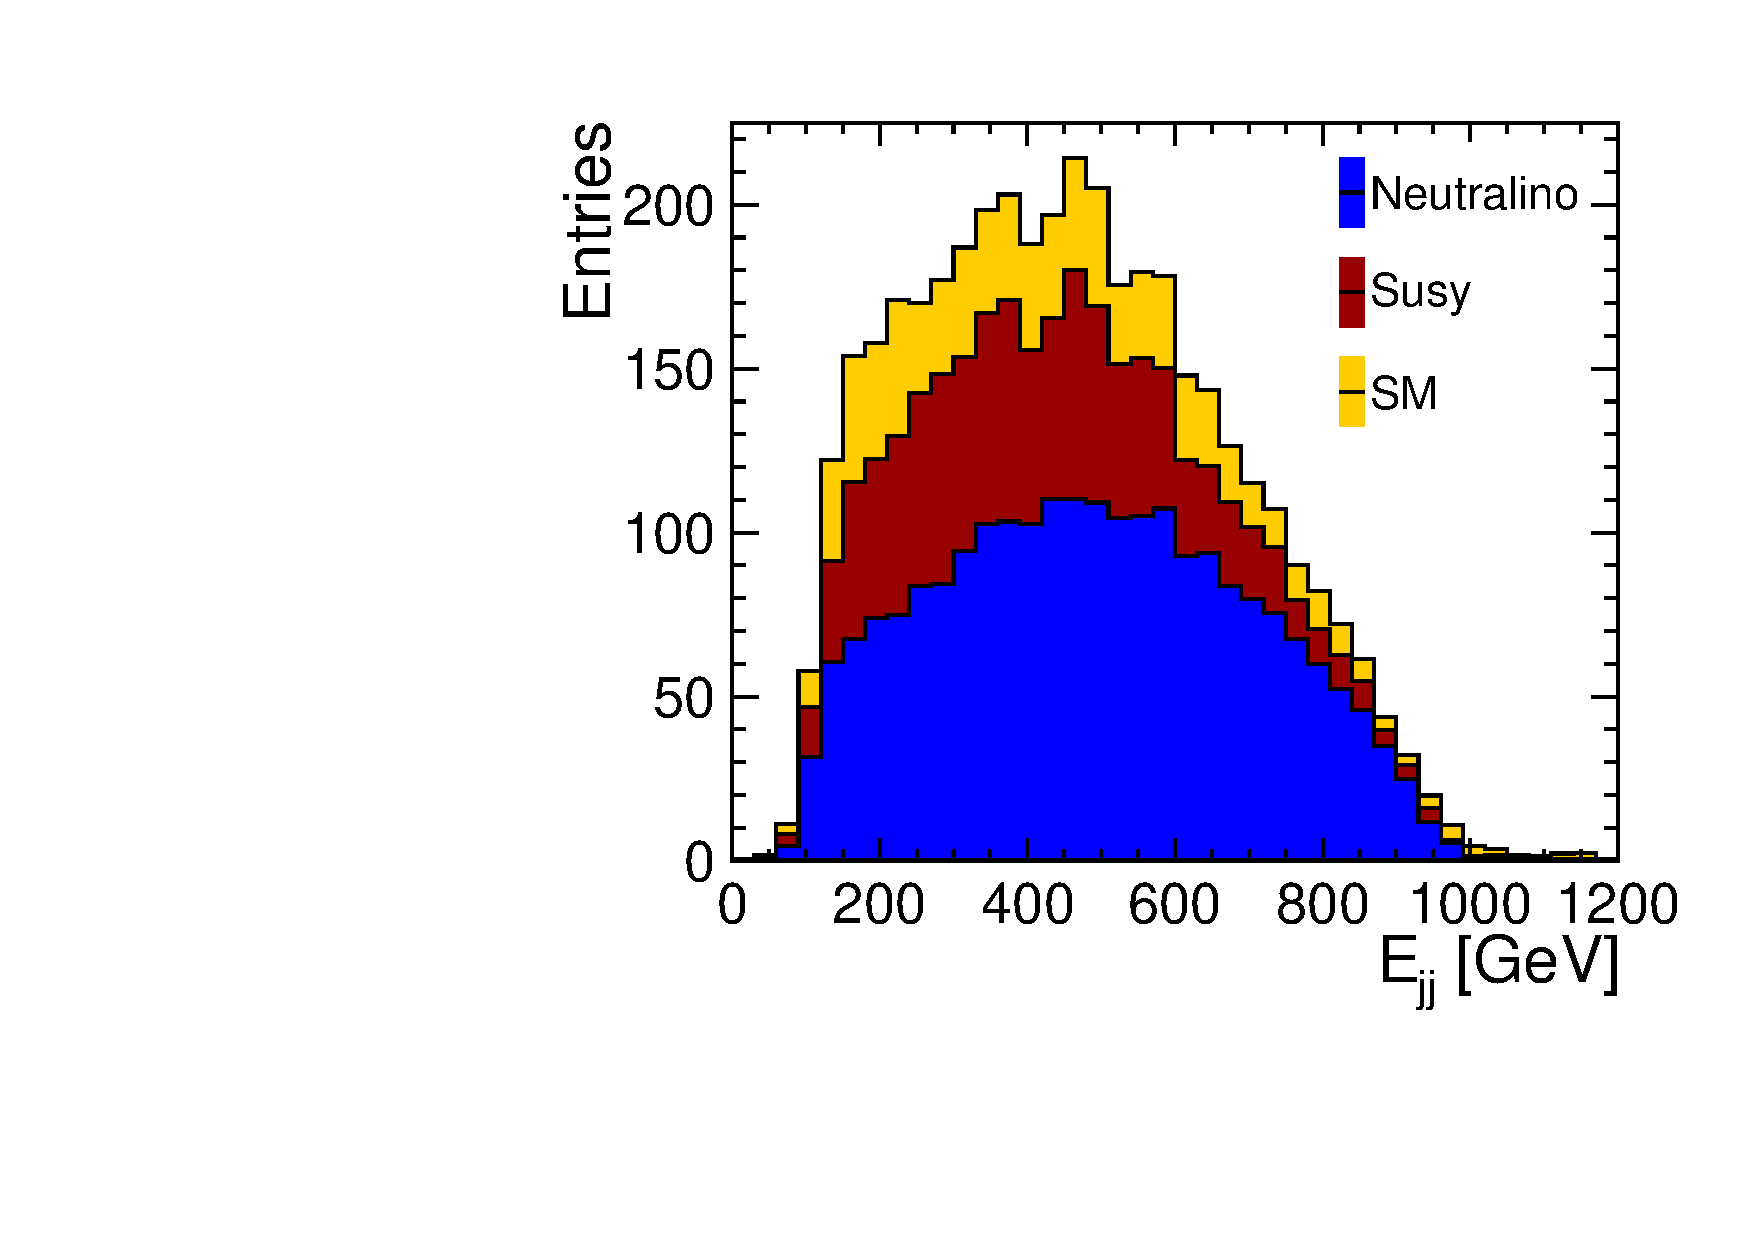
\includegraphics[width=4.5cm]{../SIDWorkshop/NeutralinoSel_E.pdf}\\
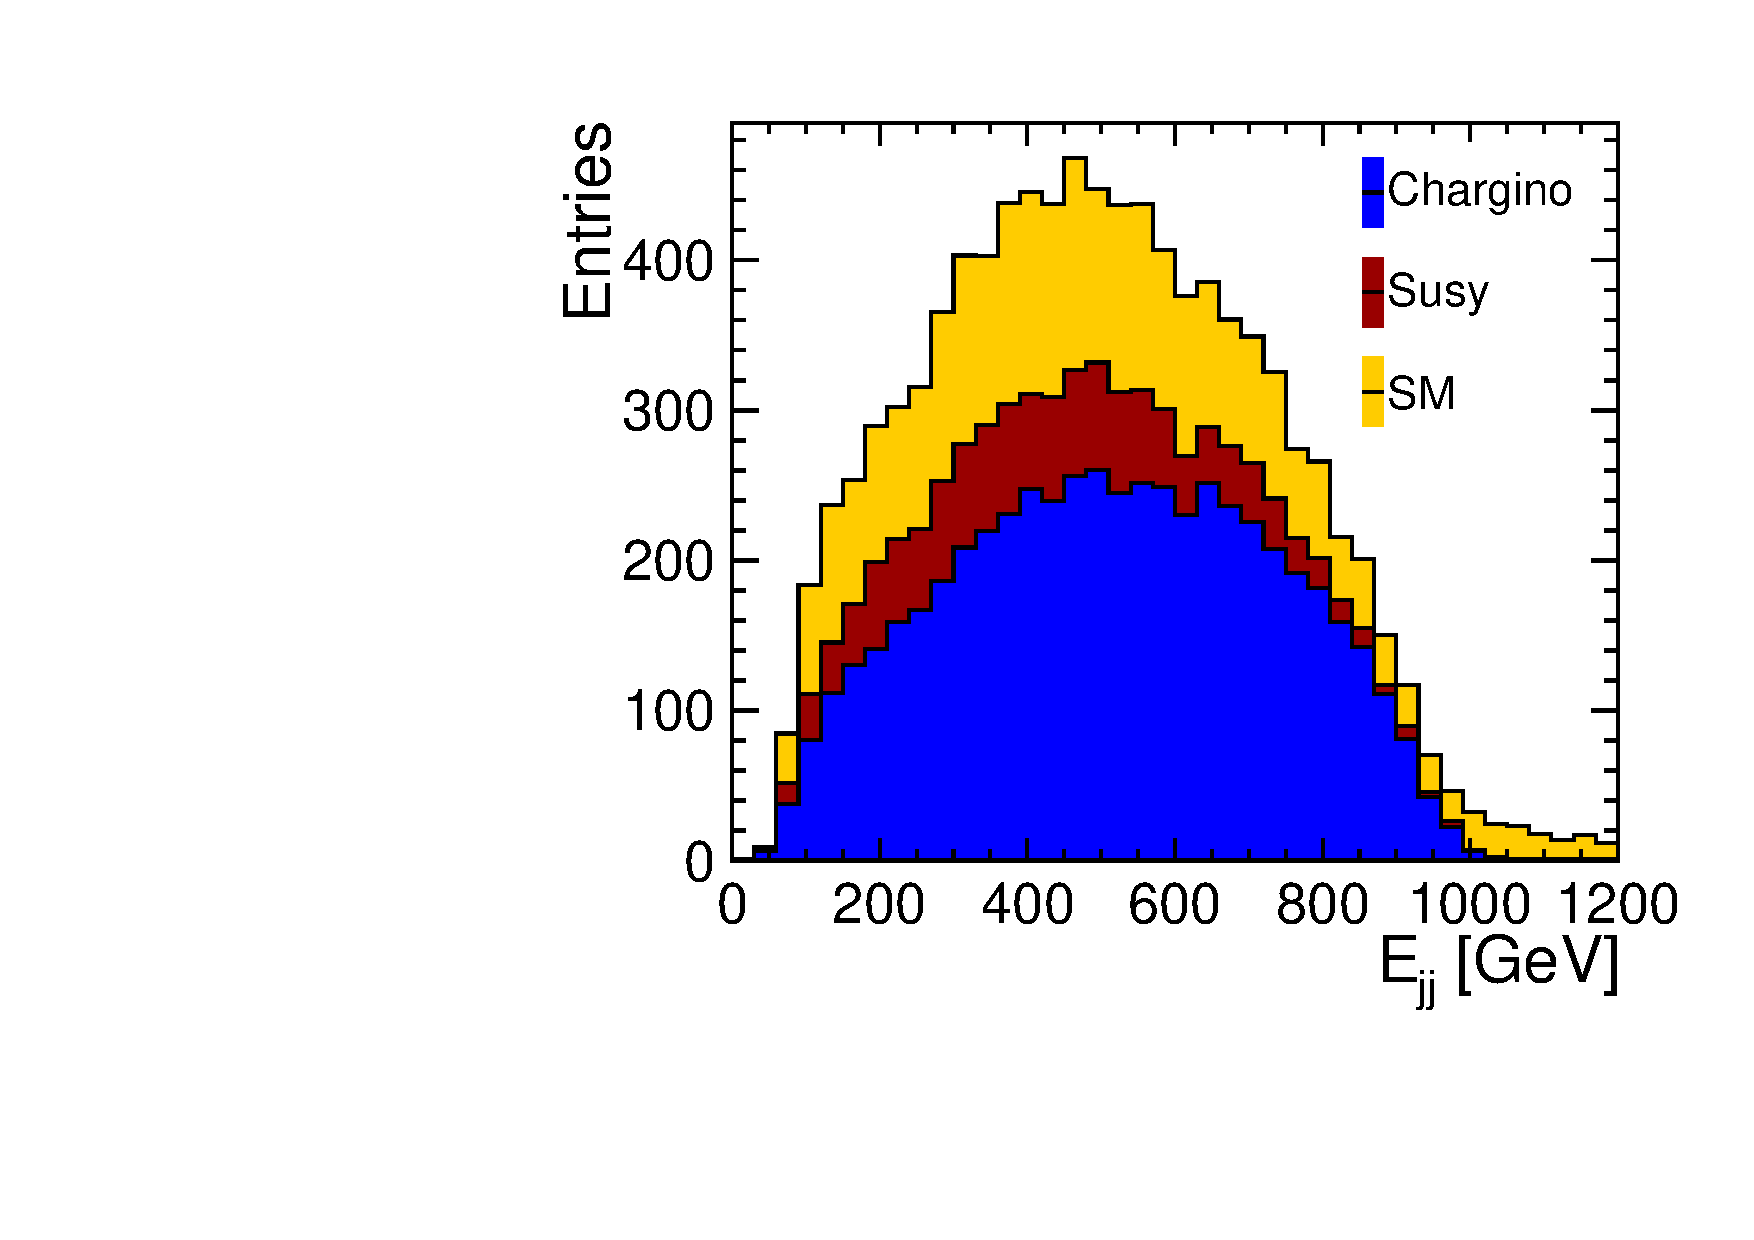
\includegraphics[width=4.5cm]{../SIDWorkshop/CharginoSel_E.pdf}
\column{4.5cm}
\centering
\includegraphics[width=4.5cm]{../SIDWorkshop/NeutralinoSel_M.pdf}\\
\includegraphics[width=4.5cm]{../SIDWorkshop/CharginoSel_M.pdf}
\end{columns}
\end{frame}
\begin{frame}
\frametitle{Gauginos}
\begin{center}
\begin{tabular}{c c c c}
       \toprule
       Parameter 1                & Uncertainty &          Parameter 2 & Uncertainty \\
       \midrule
       $M(\tilde{\chi}_{1}^{\pm})$ & $6.3$~GeV & $\sigma(\tilde{\chi}_{1}^{+}\tilde{\chi}_{1}^{-})$  & $2.2$\% \\
       $M(\tilde{\chi}_{1}^{0})$   & $3.0$~GeV & $\sigma(\tilde{\chi}_{1}^{+}\tilde{\chi}_{1}^{-})$  & $1.8$\% \\
       $M(\tilde{\chi}_{2}^{0})$   & $7.3$~GeV & $\sigma(\tilde{\chi}_{2}^{0}\tilde{\chi}_{2}^{0})$  & $2.9$\% \\
\end{tabular}
\end{center}
\end{frame}


%\begin{frame}
%\frametitle{Top physics at 500GeV: vertex detector}
%\end{frame}
\begin{frame}
\frametitle{Top physics at 500 GeV}
{\footnotesize Needed change in design of the vertex detector region}\\
~\\
\begin{columns}[c]
\column{6cm}
\centering
Semi-leptonic decay:\\ 
\includegraphics[width=5cm]{../SIDWorkshop/FinalFit-SemiLeptonic}\\
{\scriptsize
\begin{tabular}{c c }
\toprule
Top mass (GeV) & Top width (GeV)\\
\midrule
$174.28 \pm 0.09$ &  $1.55 \pm 0.26$
\end{tabular}}
\column{6cm}
\centering
Fully-hadronic decay:
\includegraphics[width=5cm]{../SIDWorkshop/FinalFit-FullHadronic}\\
{\scriptsize
\begin{tabular}{c c }
\toprule
Top mass (GeV) & Top width (GeV)\\
\midrule
$174.07 \pm 0.08$ &  $1.33 \pm 0.22$
\end{tabular}}
\end{columns}
\end{frame}

\section{Conclusion}
\begin{frame}
\frametitle{Overview}
\begin{itemize}
  \item Introduced the CLIC machine
  \item Presented the CLIC detectors concept
  \item Assessment of the physics potential of a future multi-TeV $\Pep\Pem$
  collider was made, specificaly at 3TeV
  \item Physics signals with mass scale $100-1500$GeV can be extracted with good
  precision
  \item Shown that it's possible to deal with the beam-induced background
  \item CDR physics and detector study part of a world-wide effort, broad
  international participation
  \item Further in-depth studies and hardware R\&D for the CLIC detectors are
  forseen: more detailed simulation, different c-m-e studied
  \item Follow up of LHC results
\end{itemize}
\end{frame}
\begin{frame}
\frametitle{Signatory list}
\textit{You are cordially invited to subscribe to the CDR Signatories List:\\
\begin{itemize}
\item If you have made contributions to the CLIC accelerator or the Linear
Colliders Physics and Detector studies, or intend to contribute in the future,
\end{itemize}
~\\
OR / AND\\
~\\
\begin{itemize}
  \item If you wish to express support to the physics case and the study of a
  multi-TeV Linear Collider based on the CLIC technology, and its detector
  concepts.
\end{itemize}
}
\url{https://indico.cern.ch/conferenceDisplay.py?confId=136364}
\end{frame}

\appendix
\section{Backup}
\begin{frame}
\frametitle{Backup slides}
\end{frame}
\section{Software}
\begin{frame}
\frametitle{Generation}
Use WHIZARD:
\begin{itemize}
  \item Computes proper matrix elements at tree level (OMEGA)
  \item Explicit up to 6 fermion final states
  \item Handles SUSY (LesHouches)
  \item Writes out stdhep (format used for simulation)
  \item Common for the 2 detectors
\end{itemize}
Use PYTHIA for $\Ptop\APtop$, $WW$, $ZZ$ as final states in WHIZARD have no
width
\end{frame}
\begin{frame}
\frametitle{Simulation}
2 detectors $\to$ 2 sim software
\begin{itemize}
  \item Mokka (ILD): Calls G4, Detector geometry obtained from MySQL DB
  (\alert{!!})
  \item SLIC (SiD): wrapper around G4, detector geometry imported using compact
  XML
  \item Both use the LCIO event format
\end{itemize}
Frameworks are going to be merged eventually, work ongoing
\end{frame}
\begin{frame}
\frametitle{Handling background in the software}
$\gamma\gamma$ bkg overlayed on top of simulated events\\
\begin{itemize}
  \item Simulate the bkg separately
  \item For 1 signal event, read N events of bkg (Poisson distribution,
  $\mu=3.2$) $\times$ 60 BX
  \item Merge the clusters
  \item Save the resulting collections (containers)
\end{itemize}
\end{frame}
\begin{frame}
\frametitle{Reconstruction}
As for simulation: 2 frameworks
\begin{itemize}
  \item Marlin (ILD): C++
  \item \texttt{org.lcsim}: JAVA
  \item Usual modular algorithm/tools structure (e.g. GAUDI)
  \item Use the LCIO event format
\end{itemize}
\end{frame}
\begin{frame}
\frametitle{Using the GRID: ILCDIRAC}
Grid production tool based on DIRAC
\begin{itemize}
  \item Extented to fit the CLIC study use case: application handling, data,
  etc.
  \item $>4$million jobs in 1 year
  \item Now also used for the ILC\_SiD studies
\end{itemize}
\end{frame}

\section{CLIC}
\begin{frame}
\frametitle{Accelerator complex}
\includegraphics[width=11cm]{cliccomplex.png}
\end{frame}
\begin{frame}
\frametitle{CLIC numerical properties}
\begin{center}
\begin{tabular}{rl}
Acceleration field & 100MV/m\\
RF frequency of the main linac & 12GHz\\
Beam focusing at IP & 68$\mu$m\\
Charge per bunch & $3.7\times10^9$\\
Bunch interval & 0.5 ns\\
Bunch per train & 312\\
Linac repetition rate & 50Hz\\
Beam power & 14MW\\
Normalized vertical emittance & $2\times10^{-8}$mrad\\
Vertical beam size (IP) & 1nm\\
Horizontal beam size (IP) & 40nm\\
Total power consumption & 560MW
\end{tabular}
\end{center}
\end{frame}
\begin{frame}
\frametitle{Luminosity spectrum}
\includegraphics[width=10cm]{Lumi3TeV_fixed_nopeak.pdf}
Lumi in top 1\%: $2.0\times10^{34}$cm$^{-2}$s$^{-1}$, full lumi
$5.9\times10^{34}$cm$^{-2}$s$^{-1}$
\end{frame}
\begin{frame}
\frametitle{Beam-induced background}
\includegraphics[width=5.5cm]{Energy.pdf}
\includegraphics[width=5.5cm]{Angle.pdf}\\
Beam halo muons estimated to be $\sim1$ per 20 BX: neglected
\end{frame}
\begin{frame}
\frametitle{Beam Polarization}
Not studied in this document, planned for volume 3.\\
Polarized electron beam up to 80\%.\\
Polarized positron beam $\sim30\%$ planned for a later stage
\end{frame}

\section{Physics potential}
\begin{frame}
\frametitle{Higgs production}
\begin{center}
\includegraphics[width=9cm]{higgs_production.pdf}\\
\includegraphics[width=5cm]{xsec_vs_Hmass_sqrts500.pdf}
\includegraphics[width=5cm]{xsec_vs_Hmass_sqrts3000.pdf}
\end{center}
\end{frame}
\begin{frame}
\frametitle{Higgs sensitivity}
\begin{itemize}
  \item $g_{\PH\to\mu\mu}$: 15\% for 4 years
  \item  $g_{\PH\to\Pbottom\APbottom}$: 0.22\% on $\sigma\times B$. Theoretical
  uncertainties are dominating: $\pm2-4\%$
  \item $g_{\PH\to\Pcharm\APcharm}$: $3.24\%$ on $\sigma\times B$. With
  theoretical uncertainty: $\pm3-6\%$
\end{itemize}
Other searches:
\begin{itemize}
  \item Trilinear couplings: $\Pep\Pem\to\nu_e\bar{\nu_e}HH$ (WW fusion)
  \item Anomalous Higgs couplings
\end{itemize}
\end{frame}

\begin{frame}
\frametitle{SUSY Models}
\includegraphics[width=5.5cm]{../SIDWorkshop/susy_model1.png}
\includegraphics[width=5.5cm]{../SIDWorkshop/susy_model2.png}\\
Precise measurement of fundamental parameters\\
Tests of the high-scale structure of the theory (GUT)\\
Testing the neutralino dark matter hypothesis
\end{frame}

\section{Detector requirements}
\begin{frame}
\frametitle{Track momentum resolution}
\includegraphics[width=5.5cm]{higgs.pdf}
\includegraphics[width=5.5cm]{higgs_mumu_momres_dependence_2ab.pdf}
\end{frame}
\begin{frame}
\frametitle{Jet energy resolution}
\includegraphics[width=5.5cm]{wzSeparation.pdf}
\includegraphics[width=5.5cm]{SquarkEndpoint.pdf}
\end{frame}

\section{Detector design}
\begin{frame}
\frametitle{Vertex detector}
\includegraphics[width=5.5cm]{occupancies-barrel.pdf}
\includegraphics[width=5.5cm]{vtx-ftd-hit-density.pdf}
\end{frame}

\begin{frame}
\frametitle{Tracking detectors: ILD TPC}
\includegraphics[width=5.5cm]{AngularCoverageCLIC_ILD.pdf}
\includegraphics[width=5.5cm]{CLIC_ILD_X0.pdf}
\end{frame}
\begin{frame}
\frametitle{Occupancy in the TPC}
\includegraphics[width=5.5cm]{TPCoccupancies.pdf}
\includegraphics[width=5.5cm]{TPCoccupancies_1mmPads.pdf}
\end{frame}
\begin{frame}
\frametitle{Tracking performance in the TPC}
\begin{columns}[c]
\column{8cm}
\begin{center}
\includegraphics[width=4cm]{CDRStyle_SingleMuons_MomRes_Vs_PT.pdf}
\includegraphics[width=4cm]{CDRStyle_SingleMuons_MomRes_Vs_Theta.pdf}\\
Single muons
\end{center}
\column{4cm}
\begin{center}
\includegraphics[width=4cm]{pt_resolution_ttbar_LDC_CDR.pdf}\\
$\Ptop\APtop$ events
\end{center}
\end{columns}
~\\
~\\
\begin{columns}[c]
\column{5cm}
\begin{displaymath}
\sigma(\Delta p_{\textrm{T}}/p_{\textrm{T}}^2) = a \oplus \frac{b}{p\sin\theta}
\end{displaymath}
\column{5cm}
\begin{tabular}{c r r}
\toprule
  $\theta$ \footnotesize{[$^{\circ}$]} & $a$
  \footnotesize{$[\mathrm{GeV}^{-1}]$} & $b$ \\\midrule 
  10 & $8.19\cdot10^{-4}$ & $9.07\cdot10^{-3}$ \\
        20 & $9.86\cdot10^{-5}$ & $3.83\cdot10^{-3}$ \\
        30 & $3.87\cdot10^{-5}$ & $1.59\cdot10^{-3}$ \\
        80 & $1.97\cdot10^{-5}$ & $7.22\cdot10^{-4}$ \\\bottomrule
\end{tabular}
\end{columns}

\end{frame}

\begin{frame}
\frametitle{Tracking detectors: SiD silicon layers}
\includegraphics[width=5.5cm]{CLIC_SiD_layers.pdf}
\includegraphics[width=5.5cm]{CGrefe_Fig6.pdf}
\end{frame}
\begin{frame}
\frametitle{Tracking performance in CLIC\_SiD}
\begin{columns}[c]
\column{6cm}
\includegraphics[width=5.5cm]{sid_singleMuonMomentumRes.pdf}
\column{5cm}
\begin{tabular}{r r r}\toprule
$\theta$ \footnotesize{$\left[ ^{\circ}\right]$} & $a$
\footnotesize{$\left[\mathrm{GeV}^{-1}\right]$} & $b$\\\midrule 90 & $7.3\cdot10^{-6}$ & $2.0\cdot10^{-3}$ \\
30 & $1.9\cdot10^{-5}$ & $3.8\cdot10^{-3}$ \\
10 & $4.0\cdot10^{-4}$ & $5.3\cdot10^{-3}$ \\\bottomrule
\end{tabular}
\end{columns}
\end{frame}

\begin{frame}
\frametitle{Calorimetry}
\begin{center}
\begin{tabular}{cccc}\toprule
Material & $\lambda_{\textrm{I}}$ [cm] & $\textrm{X}_0$ [cm] &
$\lambda_{\textrm{I}}/\textrm{X}_0$ \\ 
\midrule Fe       & 16.77             & 1.76       & 9.5\\
W        & 9.95              & 0.35       & 28.4\\ \bottomrule
\end{tabular}\\
~\\
\includegraphics[width=7cm]{Fig81.pdf}
\includegraphics[width=4cm]{ildHcal_jetEnergyResolution_vs_hcalLambdaI.pdf}
\end{center}
\end{frame}

\begin{frame}
\frametitle{Timing}
\includegraphics[width=5.5cm]{timingKL_steel.pdf}
\includegraphics[width=5.5cm]{timingKL_tungsten.pdf}
\end{frame}

\begin{frame}
\frametitle{CALICE results}
\begin{center}
\includegraphics[width=7cm]{RPC_Fig1.pdf}\\
\begin{columns}[c]
\column{5.5cm}
\begin{tikzpicture}
\node [] {\includegraphics[width=5.5cm]{ResolutionFullDet2Curves.pdf}};
\node [] at (0.7,0.6) {AHCAL/Tungsten};
\end{tikzpicture}
\column{5.5cm}
\begin{tikzpicture}
\node [] {\includegraphics[width=5.5cm]{RPC_Fig2.pdf}};
\node [] at (-0.5,-1.0) {DHCAL/Steel};
\end{tikzpicture}
\end{columns}
\end{center}
\end{frame}
\begin{frame}
\frametitle{Calorimeter performance}
\begin{center}
\includegraphics[width=4.7cm]{Eres_vsE_ILD.pdf}
\includegraphics[width=4.7cm]{Eres_vsE_SID.pdf}\\
\includegraphics[width=4.7cm]{Eres_vsThetaStripped_ILD.pdf}
\includegraphics[width=4.7cm]{Eres_vsThetaStripped_SID.pdf}
\end{center}
\end{frame}
\begin{frame}
\frametitle{Resolution vs timing in calorimeter}
\begin{center}
\includegraphics[width=7cm]{Eres_Timing_ILD.pdf}
\end{center}
\end{frame}

\begin{frame}
\frametitle{Magnets}
\begin{center}
{\scriptsize
  \begin{tabular}{l c c c c } \toprule
             & Nominal magnetic field & Free bore & Magnetic length & Cold mass weight \\
             & (T)                    & (mm)      & (mm)            & (tons)           \\\midrule
    CLIC\_SiD & 5.0                    & 5480      & 6230            & 170   \\          
    CLIC\_ILD & 4.0                    & 6850      & 7890            & 210             
    \\\bottomrule
  \end{tabular}
  }
  \end{center}
\begin{itemize}
  \item Similar to the CMS solenoid in design
  \item Aluminium stabilized superconductor
  \item Multi-layer and multi-module coil
  \item Helium cooling
\end{itemize}
\end{frame}

\begin{frame}
\frametitle{Muon system}
Installed in the return yoke of the magnet
\begin{center}
\includegraphics[width=5.5cm]{MS_SiD_HG.pdf}
\end{center}
\end{frame}
\begin{frame}
\frametitle{Muon system}
\begin{center}
\includegraphics[width=11cm]{effPur_MuonsInZbb_and_muonGunE150pm150_defaultCuts.pdf}
\end{center}
\end{frame}

\begin{frame}
\frametitle{Very forward calorimeters: LumiCal and BeamCal}
\begin{itemize}
  \item LumiCal: measurement of the luminosity
  \item BeamCal: fast estimation of the luminosity and tagging of high energy
  electrons
\end{itemize}
Both are electromagnetic sampling calorimeters, using W as absorber
\begin{center}
\includegraphics[width=7.5cm]{MDI_layout_v3.pdf}
\end{center}
\end{frame}

\section{Benchmarking the detector}
\begin{frame}
\frametitle{Luminosity spectrum measurement}
\includegraphics[width=5.5cm]{Spectra_BHWide_noEsmearing_full.pdf}
\includegraphics[width=5.5cm]{Spectra_BHWide_noEsmearing_zoom.pdf}\\
Impact on physics observable very small.
\end{frame}

\begin{frame}
\frametitle{Particle ID performance}
\begin{columns}[c]
\column{5.5cm}
\begin{center}
\begin{tikzpicture}
\node [] {\includegraphics[width=4.5cm]{ILDElectronsEffVsEnergy.pdf}};
\node [] at (0,-1) {Electrons};
\end{tikzpicture}
\begin{tikzpicture}
\node [] {\includegraphics[width=4.5cm]{ILDPionsEffVsEnergy.pdf}};
\node[] at (0,-1) {Pions};
\end{tikzpicture}
\end{center}
\column{5.5cm}
\begin{center}
\begin{tikzpicture}
\node [] {\includegraphics[width=4.5cm]{ILDGAMMAEffVsEnergy.pdf}};
\node [] at (0,-1) {Photons};
\end{tikzpicture}
\begin{tikzpicture}
\node [] {\includegraphics[width=4.5cm]{ILDPionsEffVsTheta.pdf}};
\node[] at (0,-1){Pions};
\end{tikzpicture}
\end{center}
\end{columns}
\end{frame}

\begin{frame}
\frametitle{Particle ID performance: Muons}
\includegraphics[width=5.5cm]{SIDMuonsEffVsEnergy.pdf}
\includegraphics[width=5.5cm]{SIDMuonsEffVsTheta.pdf}
\end{frame}

\begin{frame}
\frametitle{Electron energy resolution}
Effect of the $\gamma\gamma$ background:
\includegraphics[width=5.5cm]{213_H1DPVOPV2A_BX060SEL1.pdf}
\includegraphics[width=5.5cm]{213_H1DPVOPV2A_BX060SEL4.pdf}
Core: $\Delta E/E^2=\sim 1.5 \times 10^{-5}$GeV$^{-1}$\\
Tails:  $\Delta E/E^2=5-8 \times 10^{-5}$GeV$^{-1}$\\
Bump due to failure in recovering the Bremstrahlung and FSR photons
\end{frame}
\begin{frame}
\frametitle{Effect of $\gamma\gamma$ bkg}
\includegraphics[width=5.5cm]{PFOSelComp_SID_E500_energy_ALL.pdf}
\includegraphics[width=5.5cm]{WW_Eres_SID.pdf}
\end{frame}
\begin{frame}
\frametitle{Primary vertex position resolution}
\includegraphics[width=5.5cm]{Primary_Vertex_Position_XY.pdf}
\includegraphics[width=5.5cm]{Primary_Vertex_Resolution.pdf}
\end{frame}

\begin{frame}
\frametitle{Flavour tagging}
LCFI collaboration, uses ZVTOP vertex finder and multi-variate method (NNET)\\
\includegraphics[width=5.5cm]{Invariant_Mass_All.pdf}
\includegraphics[width=5.5cm]{B_Flavour_Tag_Sum.pdf}
\end{frame}
\begin{frame}
\frametitle{Flavour tagging}
\begin{center}
\begin{tabular}{l r r}
        \toprule
        & \textbf{$\PH\to \Pbottom\APbottom$} & \textbf{$\PH\to
        \Pcharm\APcharm$}
        \\
        \midrule
%        Signal events       & $311\times10^3$ & $395\times10^1$    \\
%        Total signal events & $570\times10^3$ & $260\times10^2$     \\
%        Background events   & $165\times10^3$ & $124\times10^3$\\
        Signal purity       & 65.4\% & 24.1\%  \\
        Signal efficiency   & 54.6\% & 15.2\%  \\
        % Cross section $\sigma_{\PSh\,\to\,\qqbar}$ & 285~fb & 13~fb \\
        cross section & & \\statistical uncertainty   & 0.22\% & 3.24\% \\
        \bottomrule
    \end{tabular}
    \end{center}
\end{frame}

\end{document}